\documentclass[a4paper,openany]{book}
\usepackage[paperwidth=18cm]{geometry}
\usepackage{layouts}
\printinunitsof{cm}
\usepackage{graphicx}
\usepackage{natbib}
\usepackage{amsmath}
\usepackage{amsfonts}
\usepackage{float}
\usepackage{caption}
\usepackage{wasysym}
\usepackage{tikz}
\usepackage{float}
\usepackage{subcaption}
\usepackage{makecell}
\usepackage[title]{appendix}
\usepackage{longtable}
\usepackage{cprotect}
\usepackage{cleveref}
\DeclareMathOperator{\Tr}{Tr}
\DeclareMathOperator{\spn}{span}
\newcommand{\minus}{\scalebox{0.75}[1.0]{$-$}}
\begin{document}
\begin{center}

\title{Discontinuous Galerkin method for direct numerical simulation of the Navier Stokes equation: Master Thesis Report}


\author{Nirav Vasant Shah, \\M.Sc. Candidate, Water Resources Engineering and Management, \\Universit\"at Stuttgart, \\Stuttgart, Deutschland (Germany)\\ 
\and Supervisor: Prof. Dr. Bernard Haasdonk,\\ Institute of Applied Analysis and Numerical Simulation, \\Universit\"at Stuttgart,\\ Stuttgart, Deutschland (Germany)\\ \and Co-advisor: Prof. Dr. Gianluigi Rozza,\\ Scuola Internazionale Superiore di Studi Avanzati, \\Trieste, Italy \\ \and Co-advisor: Dr. Martin Hess,\\ Scuola Internazionale Superiore di Studi Avanzati, \\Trieste, Italy }
\date{\today}
\maketitle

\end{center}

\noindent

\section{Acknowledgement}

The  presented in this thesis is a result of the work carried out between September 2017 - March 2018 at the Institute of Applied Analysis and Numerical Simulation, Universit\"at of Stuttgart and Scuola Internazionale Superiore di Studi Avanzati, Trieste. \\

Undoubtedly, this result could only be achieved by the support of a number of people to whom I would
like to express my gratitude.\\

To my supervisor Professor Bernard Haasdonk: I experienced the freedom I needed to be
creative while at the same time I was always helped to continue research in case of diffi-
culties. \\

To my coadvisors Dr. Martin Hess and Professor Dr. Gianluigi Rozza: I am thankful for their positive coordination and helping me to develop necessary skills in the field of work. \\

I am really looking forward to continue these valuable working relationships.\\

To my colleagues: I would also thank colleagues for their positive interest in my work and very positive support for the work.\\

To my parents:  Last but most importantly, I would like to thank my parents for their encouragement, infusing new energy to continue with my work.

\newpage

\section{Declaration/Eigenst\"andigkeitserkl\"arung}

I hereby certify that I have prepared this master‘s thesis independently, and that only those sources, aids and advisors that are duly noted herein have been used and / or consulted.\\
${}$\\
${}$\\
Hiermit versichere ich, dass ich die vorliegende Seminararbeit selbständig und
nur mit den angegebenen Hilfsmitteln verfasst habe. Alle Passagen, die ich
wörtlich aus der Literatur oder aus anderen Quellen wie z. B. Internetseiten
übernommen habe, habe ich deutlich als Zitat mit Angabe der Quelle kenntlich
gemacht.\\
${}$\\
${}$\\
${}$\\
${}$\\
${}$\\
Signature/Unterschrift
${}$\\
${}$\\
${}$\\
${}$\\
${}$\\
Place,Date/Ort, Datum











\newpage

\newenvironment{spmatrix}[1]
 {\def\mysubscript{#1}\mathop\bgroup\begin{pmatrix}}
 {\end{pmatrix}\egroup_{\textstyle\mathstrut\mysubscript}}

\section{List of symbols} \label{symbol_list}

Following is the list of symbols used throughtout the thesis with their respective meaning.\\
${}$\\
\begin{longtable}{| p{.35\textwidth} | p{.65\textwidth} |}
\hline
\textbf{Symbol/Abbreviation} & \textbf{Description}\\
\hline
$CFD$ & Computational Fluid Dynamics\\
\hline
$\Omega$ & Continuous domain\\
\hline
$\partial \Omega$ & Continuous domain boundary\\
\hline
$\Gamma_D$ & Dirichlet boundary\\
\hline
$\Gamma_N$ & Neumann boundary\\
\hline
$B'$ & Extensive property under consideration \\
\hline
$b'$ & Intensive property corressponding to $B'$\\
\hline
$t$ & Neumann value\\
\hline
$t'$ & time\\
\hline
$cv$ & Control volume\\
\hline
$cs$ & Control system\\
\hline
$\rho$ & Density of fluid \\
\hline
$u$ & Velocity\\
\hline
$p$ & Pressure\\
\hline
$M$ & Momentum of fluid flowing through control volume\\
\hline
$f$ & Source/Sink/External force per unit volume\\
\hline
$F$ & External force acting on $cv$\\
\hline
$\sigma$ & Stress\\
\hline
$\nu$ & Kinematic viscocity\\
\hline
$u_D$ & Velocity at Dirichlet boundary\\
\hline
$n$ & Unit normal vector pointing outward from element\\
\hline
$DNS$ & Direct Numerical Simulation\\
\hline
$\nabla^s$ & Symmetric tensor, $\frac{1}{2} (\nabla + \nabla^T)$\\
\hline
$Re$ & Reynolds number\\
\hline
$L$ & Characteristic length for Reynolds number\\
\hline
$\mathcal{T}$ & Grid or discretised domain\\
\hline
$\partial \mathcal{T}$ & Grid boundaries\\
\hline
$\Gamma$ & Interelement or internal boundary of grid\\
\hline
$nel$ & Total number of elements of grid\\
\hline
$k$ & Index of an element, $1\leq k \leq nel$\\
\hline
$n^+$ & Unit normal vector pointing from element itself to neighbouring element\\
\hline
$n^-$ & Unit normal vector pointing from neighbouring element to element itself \\
\hline
$\tau_k$ & $k^{th}$ Triangular element, $\tau_k \in \mathcal{T}$\\
\hline
$h_{\tau_k}$ & Diameter of $\tau_k$\\
\hline
$\theta_k$ & Smallest angle of $\tau_k$\\ 
\hline
$r$ & Coordinates of point in Barycentric coordinate system\\
\hline
$r_1, r_2, r_3$ & Coordinates of Vertices of triangle\\
\hline
$\lambda_1, \lambda_2, \lambda_3$ & Weights in barycentric coordinate system (Equation \ref{barycentric point})\\
\hline
$\mathbb{V}$ & Function space for velocity\\
\hline
$\mathbb{Q}$ & Function space for pressure\\
\hline
$P^D$ & Polynomial of degree $D$\\
\hline
$D$ & Polynomial degree\\
\hline
$\phi$ & Velocity basis function in global space\\
\hline
$\psi$ & Pressure basis function in global space\\
\hline
$\hat{\phi}$ & Velocity basis function in local space\\
\hline
$\hat{\psi}$ & Pressure basis function in local space\\
\hline
$N$ & Truth space dimension\\
\hline
$F_k$ & Mapping from local coordinate system to global coordinate system (Equation \ref{local global mapping equation})\\
\hline
$\hat{T}$ & Reference triangle\\
\hline
$J_k$ & Jacobian of $\tau_k$ (Equation \ref{local global mapping equation})\\
\hline
$\hat{X}$ & Coordinates of point in local coordinate system, $\hat{X} \in \mathbb{R}^d$\\
\hline
$X$ & Coordinates of point in global coordinate system, $X \in \mathbb{R}^d$\\
\hline
$C$ & Translational vector for local to global mapping (Equation \ref{local global mapping equation})\\
\hline
$g$ & Function in global space \\
\hline
$\hat{g}$ & Function in local space \\
\hline
$g^{up}$ & Upwind value of function $g$\\
\hline
$det$ & Determinant of matrix \\
\hline
$\hat{\Gamma}$ & An edge of reference Triangle $\hat{T}$\\
\hline
$JIT_k$ & Jacobian inverse transpose corresponding to $\tau_k$, $J_k^{-1}$\\
\hline
$C_{11}$ & Penalty parameter \\
\hline
$a_{IP}$ & Term representing poisson operator of strong form in weak formulation of the Navier Stoks equation (Equation \eqref{navier_stokes_weak_ch3}) \\
\hline
$b$ & Term representing gradient operator in weak formulation of the Navier Stoks equation (Equation \eqref{navier_stokes_weak_ch3})\\
\hline
$c$ & Term representing non linear terms in weak formulation of the Navier Stoks equation (Equation \eqref{navier_stokes_weak_ch3})\\
\hline
$A$ & Matrix terms corresponding to $a_{IP}$\\
\hline
$B$ & Matrix terms in corresponding to $b$\\
\hline
$C$ & Matrix terms in corresponding to $c$\\
\hline
$l_{IP}$ & Term representing right hand side of strong form in weak formulation of the Navier Stoks equation (Equation \eqref{navier_stokes_weak_ch3}) \\
\hline
$u^{ext}$ & External trace of Velocity (Equation \ref{uext})\\
\hline
$l$ & Length of an edge on $\mathcal{T}$\\
\hline
$U$ & Velocity solution vector \\
\hline
$P$ & Pressure solution vector\\
\hline
$F_1$ & Discrete form of right hand side of equatio \eqref{navier_stokes_weak_ch3}\\
\hline
$F_2$ & Discrete form of right hand side of equation \eqref{contiuity_weak_ch3}\\
\hline
$u_{ndofs}$ & Total number of degrees of freedom of Velocity\\
\hline
$p_{ndofs}$ & Total number of degrees of freedom of Pressure\\
\hline
$bicgstab$ & Biconjugate gradients stabilized method\\
\hline
$minres$ & Minimum residual method\\
\hline
$z$ & Non zero vector\\
\hline
$\lbrace \cdot \rbrace$ & Average operator\\
\hline
$[\cdot]$ & Jump operator\\
\hline
$(\cdot,\cdot)$ & $L^2$ scalar product\\
\hline
$S$ & Schur complement\\
\hline
$I$ & Identity matrix\\
\hline
$u_{npe}$ & Number of degrees of freedom per element for Velocity\\
\hline
$p_{npe}$ & Number of degrees of freedom per element for Pressure\\
\hline
$d$ & Dimension of problem\\
\hline
$\kappa_e$ & Coercivity constant\\
\hline
$k'$ & Sobolev space order\\
\hline
$w_i$ & Weight in Gaussian quadrature rule\\
\hline
$nop$ & Number of points\\
\hline
\end{longtable}
\listoffigures
\listoftables

\tableofcontents

\chapter{Introduction}

\section{Overview}

The thesis deals with the numerical simulation of the Navier Stokes equation [White F.M. \cite{white}] which is the core of Computational Fluid Dynamics or $CFD$. The thesis performs numerical simulation of the Navier Stokes equation through the discontinuous Galerkin method.

The goal of the thesis is to derive, discretise and implement the discontinuous Galerkin [Riviere B. \cite{riviere}] weak form of the Navier Stokes equation and perform numerical simulation of the Navier Stokes equation. In the course of the numerical solution we measure the computational efforts. This includes Solver performance such as run time, accuracy.

In Chapter 2, the Navier Stokes equation is introduced. We first derive the Navier Stokes equation from the conservation equation or the Reynolds transport theoreom. We discuss the flow classification and important issues related to numerical simulation of the Navier Stokes equation. 

In Chapter 3, we bring the infinite dimensional problem to a finite dimensional problem by introducing discretisation. We first introduce grid, constituents of elements and transformation between local and global geometry. Further the function spaces over the grid are discussed in which, the basis functions or the Ansatz functions, function spaces for pressure and velocity are introdued. We further introduce and discuss the weak form of the Navier Stokes equation, discrete form of the Navier Stokes equation with boundary conditions and properties of the weak form.

In Chapter 4, we discuss the implementation of the discrete form of the Navier Stokes equation in RBmatlab, an opensource software developed at the University of Stuttgart and the University of M\"unster, for numerical simulation. During the chapter we discuss evaluation of basis functions in RBmatlab, matrix assembly, dimension of assembled matrices and boundary condition implementation. We further discuss the Schur complement method and the Newton method for nonlinearity.

In Chapter 5, we present results from numerical experiments, analyse results from benchmark problems, evaluate solver performance and draw related conclusions.

In Chapter 6, we derive conclusions from numerical experiment results and also point towards future perspectives and possibilities for further developments.

In appendix, we present mathematical preliminaries. Familiarity with concepts presented under this chapter is very helpful for understanding of the thesis. Readers familiar with the topics can skip this section. Additionally we also provide reference to published literature, online resources and implementation used for the present analysis for readers interested in exploring the topic further.

\newpage

\chapter[Perspective and formulation]{Engineering perspective and mathematical formulation} 

The subject of mathematical applications in fluid mechanics starts with  one of the variants of the Navier Stokes equation. Almost all processes of fluid mechanics require considerations related to the Navier Stokes equation. Hence the importance of the Navier Stokes equation is impossible to be ignored as far as mathematical approaches in fluid mechanics are concerned. The numerical method for the incompressible Navier Stokes equation is simpler as compared to the numerical method for the compressible Navier Stokes equation. As the incompressible condition is imposed the state variables are constant. This in turn means that the equation of state no longer needs to be solved. Throughout the thesis we discuss only steady state incompressible Navier Stokes equation and hence, Navier Stokes equation refers hereafter to steady state incompressible Navier Stokes equation.

\section[Derivation]{Derivation of the Navier Stokes equation}

Before deriving the Navier Stokes equation we introduce some notations. The domain is denoted by $\Omega \subseteq \mathbb{R}^d $. The domain boundary is denoted by $\partial \Omega$. The domain boundary is divided into Dirichlet boundary $\Gamma_D$ and Neumann boundary $\Gamma_N$ i.e. $\Gamma_D \cup \Gamma_N = \partial \Omega $, $\Gamma_D \cap \Gamma_N = \emptyset $. 

The governing equations for the incompressible Navier Stokes flow are the conservation equations: Mass conservation and Momentum conservation. The conservation equations are derived based on the concept of control volume and the control surface. The control volume is the volume, fixed or moving with constant velocity in space, through which the fluid moves. The control surface is the surface enclosing the control volume. All equations can be derived from the Reynold's transport equation as presented by White F.M. \cite{white}:


\begin{equation} \label{rtt} 
\frac{dB'}{dt'}|_{cs} = \frac{d}{dt'} \int_{cv} b' \rho dV + \int_{cs} (b' \rho) u\cdot dA 
\end{equation}

\begin{center}
$cv$ = Control volume\\
$cs$ = Control surface\\
$B'$ = Extensive property under consideration  \\
$b'$ = Intensive property corresponding to $B'$ \\
$\rho$ = Density of fluid \\
$u$ = Velocity of fluid\\
\end{center}

If in the above equation $B'$ is substituted as momentum $M$, correspondingly $b'$ as velocity $u$, we obtain the change in momentum. As per Newton's second law of motion change in momentum is equal to the sum of external forces acting on the system. 

\begin{equation}\label{External force lhs}
F = \frac{dM}{dt'} = \frac{d}{dt'} \int_{cv} u \rho dV + \int_{cs} (u \rho) u\cdot dA 
\end{equation}

This sum of forces arises from stresses $\sigma$ (shear stresses and normal stresses) and external force $f$ such as weight. 

\begin{equation}\label{External force rhs}
F = \int_{cs} \sigma \cdot dA + \int_{cv} \rho f dV
\end{equation}
\\
$\sigma =$ Viscous stress\\
$f =$ External force per unit volume\\

Equating external forces with change in momentum i.e. equating \eqref{External force lhs} and \eqref{External force rhs}, considering steady conditions only, using definition of viscous stress tensor and with the application of the Gauss divergence theorem we arrive at the Navier Stokes equation,

\begin{equation} \label{navier_stokes}
-2\nabla \cdot (\nu \nabla^s u) + (1/\rho) \nabla p + (u \cdot \nabla)u = f \quad   \textnormal{in}  \quad \Omega \quad \textrm{.}
\end{equation} 

The incompressible mass conservation equation can be derived similarly by substituing $B' =$ Mass of control system and $b' = 1$ in equation \eqref{rtt}.  It can be written as,

\begin{equation}\label{mass_conservation}
\nabla \cdot u=0 \quad   \textnormal{in}  \quad \Omega \quad \textrm{.}
\end{equation}

The boundary conditions are expressed as,\\

Dirichlet boundary:
\begin{equation}\label{dirichlet_ns}
u=u_D \quad \textnormal{on} \quad \Gamma_D \quad \textrm{.}
\end{equation}

Neumann boundary:
\begin{equation} \label{neumann_ns}
-pn + 2\nu(n \cdot \nabla^s)u = t \quad   \textnormal{on}  \quad \Gamma_N \quad \textrm{.}
\end{equation}

$ $\\
$u$ = flow velocity and $u:\Omega \rightarrow \mathbb{R}^d$ \\
$p$ = pressure and $p:\Omega \rightarrow \mathbb{R}$\\
$\nu$ = kinematic viscocity (fluid property) $\nu:\Omega \rightarrow \mathbb{R}$\\ 
$\rho$ = density (fluid property) $\rho:\Omega \rightarrow \mathbb{R}$\\
$f$ = external force $f:\Omega \rightarrow \mathbb{R}^d$\\
$u_D$ = specified flow velocity at Dirichlet boundary $u_D:\Gamma_D \rightarrow \mathbb{R}^d$\\
$n$ = normal unit vector $n:\partial \Omega \rightarrow \mathbb{R}^d$\\
$t$ = specified Neumann flux $t:\Gamma_N \rightarrow \mathbb{R}^d$\\
$\nabla^s = \frac{1}{2}(\nabla + \nabla^T)$\\


The equation \eqref{navier_stokes} is known as the strong form of the Navier Stokes equation.

It can be seen that the steady state Navier Stokes equation is nonlinear and has two unknown variables, pressure $p$ and velocity $u$. The additional equation, mass conservation equation, is hence necessary to obtain a sufficient number of equations for the number of unknowns.

We also introduce the dimensionless number Reynolds number, $Re$ which is the most characteristic quantity of the flow. The Reynolds number is defined as the ratio of inertial force to the viscous force,

\begin{equation} \label{reynolds_number}
Re =  u L / \nu
\end{equation}

Where, $L$ is the Characteristic geometrical dimension, for example the diameter of a pipe in case of pipe flow or the span of the wing of an aircraft in case of flow over an aircraft wing.\\

\subsection[DNS]{Direct numerical simulation} 

We now differentiate between the type of flows, laminar and turbulent.\\

Laminar flow is characterised by well defined velocity and pressure field and low Reynolds number. This flow has very low velocity fluctuations and pressure fluctuations. The viscous force is balanced by the pressure force and the flow has negligible inertial force. Mathematically, the non linear term in \eqref{navier_stokes} is no longer present. This equation is known as Stokes equation [White F.M.\cite{white}]\\

The strong form of Stokes equation is as follow,

\begin{equation} \label{stokes_strong_form}
-\nu \Delta u + \nabla p = f \quad \textrm{in} \quad \Omega
\end{equation}

\begin{equation} \label{dirichlet condition stokes}
u = u_D \quad \textrm{on} \quad \Gamma_D
\end{equation}

\begin{equation} \label{neumann condition stokes}
-pn + \nu n \cdot \nabla u = t \quad \textrm{on} \quad \Gamma_N
\end{equation}
\\

Turbulent flow, in contrast, is characterised by fluctuations in velocity and pressure field and a high Reynolds number. The flow has high velocity and an inertial force is present in addition to a viscous and a pressure force. This inertial force makes the Equation \eqref{navier_stokes} non linear. The fluctuations of velocity and pressure are of the order of the Kolmogrov scale.[Kundu et al. \cite{Kundu}]\\

The method used for solving Equation \eqref{navier_stokes} numerically is known as Direct Numerical Simulation, abbreviated as DNS. The direct numerical simulation could be computationally very expensive especially in applications such as turbulent flows as the time and space grid size is of the order of the Kolmogrov scale but the time period or space dimension over which the simulation is carried out are very large. In order to avoid such computational expenses alternate models are used replacing the original model. However, the alternate model can not explain the flow physics completely. The prediction of accurate flow physics description requires economical numerical solution of \eqref{navier_stokes}. It is to be noted that the simulation of turbulent flow is always a choice of balance between accuracy of computation and computational efforts.

\chapter{Discretisation and function spaces}

\section{Grid geometry}

In numerical analysis a continuous problem is posed over finite number of degrees of freedom. We divide the original domain into smaller subdomains to have finite number of degrres of freedom. The divided domain is called grid. If the original domain is denoted by $\Omega$, we denote the grid by $\mathcal{T}$. In the present case we use triangular grid and denote each triangle as $\tau_k$ with $k$ as element index. If $nel$ is the total number of elements in the grid, $1\leq k \leq nel$. We note that $\mathcal{T} = \cup_{k=1}^{nel} \tau_k$. Each triangle is an 'Element' of the grid. The boundary betwen elements i.e. interelement boundary is denoted by $\Gamma$. In case of a grid, the boundary $\partial \mathcal{T}$ comprises of domain boundaries and interelement boundaries i.e. $\partial \mathcal{T} = \Gamma_D \cup \Gamma_N \cup \Gamma$. During discussion on jump operator and average operator we denote the element under consideration as $\tau_{h}^+$ and neighbouring element as $\tau_{h}^-$. (Figure \ref{fig:Self_neighbour})

\begin{figure}
\centering
  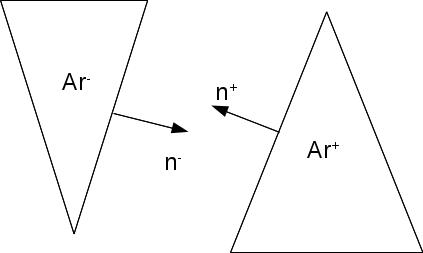
\includegraphics[width=\linewidth]{ch_3_fig_1.jpg}
  \caption{Element self (+) and neighbouring element (-)}
  \label{fig:Self_neighbour}
\end{figure}

We also denote the normal pointing from element itself towards neighbouring element as $n^+$ and the normal pointing from neighbouring element towards element itself as $n^-$. Correspondingly every quantity on element itself is denoted by superscript $+$ and on neighbouring element is denoted by $-$.  We denote by $h_{\tau_k}$ the diameter of element $\tau_k$ such that $h_{\tau_k} = \sup ||x-y||$ where, $(x,y) \in \tau_k$. We also denote by $\theta_k$ the smallest angle of the element $\tau_k$.

In case of a 2-dimensional domain the grid could be a triangular grid or a rectangular grid. The triangular grids are useful for irregular geometry and also on regular geometry if the solution is expected to be irregular due to complex flow physics. This flexibility requires additional efforts to define the grid accurately. That is, unlike a structured grid, an unstructured grid needs to define connectivity of vertices, which form edges, which in turn form a face. In case of a 2-dimensional grid we have faces which are 2-dimensional entities, edges which are 1-dimensional entities and points or vertices which are 0-dimensional entities. In case of 3-dimensional grid, these faces constitute tetrahedral elements. 

For triangular grids we also consider a barycentric coordinate system. In barycentric coordinate system any point $r$ within a triangle is expressed in terms of vertices $r_1,r_2,r_3$ forming the triangle. This is represented as, \begin{equation}\label{barycentric point}
r = \lambda_1 r_1 + \lambda_2 r_2 + \lambda_3 r_3 \quad \textrm{.}
\end{equation}

where, $\lambda_1, \lambda_2, \lambda_3$ are weights. The weights satisfy the criterion, 
\begin{equation}\label{lambda constraint} 
\lambda_1 + \lambda_2 + \lambda_3 = 1 \quad \textrm{.}
\end{equation}
Hence, we only need to specify 2 values in 2-dimensional plane in order to fully define the position of point.

For example, the centroid of triangle will have $\lambda_1 = 1/3, \lambda_2 = 1/3$. By equation \eqref{lambda constraint} we have $\lambda_3=1/3$.

\section{Grid parameters}

We refer to 'Grid parameters' as the geometrical parameters which are dependent on the geometry of the problem or the grid or both. These parameters do not depend upon the mathematical formulation but are supplementary to the mathematical formulation. On the triangular grid we have 3 entities: faces, edges, vertices as explained above. From faces we have the area (equivalent to volume of element in case of a 3-dimensional grid) and the Jacobian. As explained later in the weak form of the Stokes and Navier Stokes discontinuous Galerkin formulation and transformation between local and global geometry, the area of element is useful for volume integral terms and the Jacobian is useful for transformation between local and global geometry. From edges we derive the edge length $l$ which is useful for boundary integral terms and normal vector $n$ which is useful for flux calculation. The normal vector is the unit vector normal to the edge pointing outward from the element. Every element has 3 neighbouring elements and the element shares each of his edge with one of its neighbour. From vertices we derive the vertex index which helps to define the connectivity of the vertices which is useful especially in case of unstructured grid. In order to give clear visualization of domain or precisely, we refer to Figure \ref{fig:continuous_grid_figure}.

\begin{figure}[H]
\begin{subfigure}{.5\textwidth}
\centering
  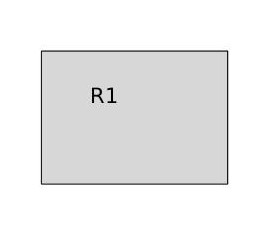
\includegraphics[width=\linewidth]{domain.jpg}
  \label{fig:Domain}
\end{subfigure}
\begin{subfigure}{.5\textwidth}	
\centering
  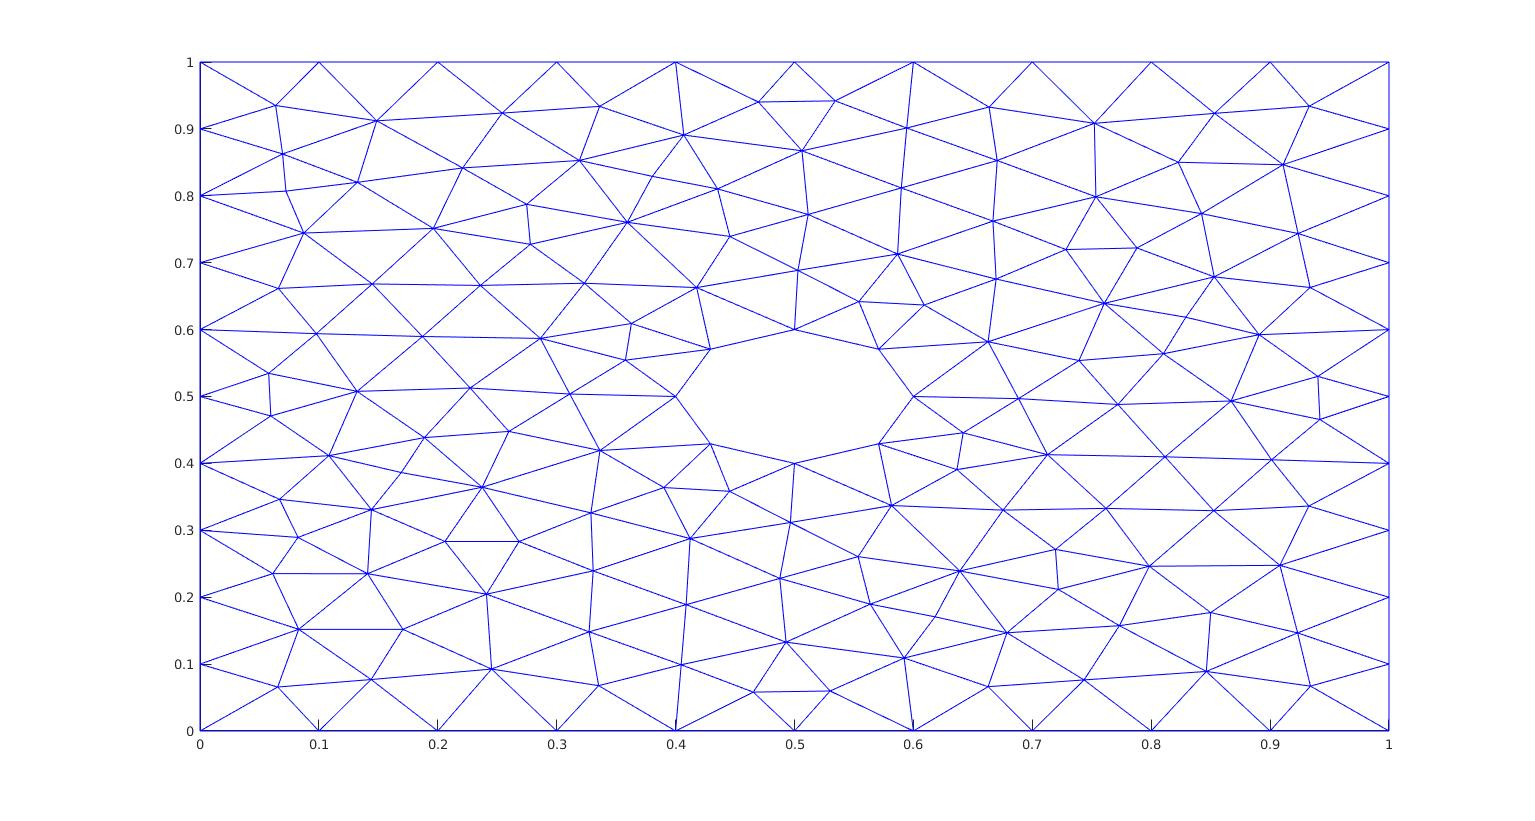
\includegraphics[width=\linewidth]{grid.jpg}
  \label{fig:Mesh}
\end{subfigure}
\caption{Continuous domain (left) and discretised domain or grid (right)}
\label{fig:continuous_grid_figure}
\end{figure}

\section{Discontinuous Galerkin method}

In the context of the discontinuous Galerkin method we introduce the function spaces $V$($\mathcal{T}$) and $Q$($\mathcal{T}$) for analytical solution of velocity and analytical solution of pressure respectively. The space containing high fidelity solution (in this case discontinuous Galerkin) is called truth space denoted by $\mathbb{V}$ for velocity and $\mathbb{Q}$ for pressure. The dimension of truth space is denoted as $N$. 

\begin{equation} \label{velocity_test}
\mathbb{V} = \lbrace \phi \in (L^2(\mathcal{T}))^{d_u}| \quad \phi \in (P^D(\tau_k))^{d_u} \quad \forall \quad {\tau_k} \in \mathcal{T} \rbrace
\end{equation}

\begin{equation} \label{pressure_test}
\mathbb{Q} = \lbrace \psi \in (L^2(\mathcal{T}))^{d_p}| \quad \psi \in (P^{D-1}(\tau_k))^{d_p} \quad \forall \quad {\tau_k} \in \mathcal{T} \rbrace
\end{equation}

Here, $P^D(\tau_k)$ denotes space of polynomials of degree at most $D$ over $\tau_k$.\\

We apply a similar procedure as in the finite element method i.e. multiplying the partial differential equation by a test function and integration by parts (Section \ref{Stokes_flow_ch3}. However, we note that our test function is not continuous on the interface. Hence, we require flux approximations and jumps at the interface. These requirements have given rise to different discontinuous Galerkin methods. For explanation of each method we refer to literatures such as by Persson et al. \cite{persson} for local discontinuous Galerkin and by Montlaur et al. \cite{Montlaur} for the Compact discontinuous Galerkin and the Interior penalty method. \\

Discontinuous Galerkin methods for the Navier Stokes equation were compared by Motlaur et al. \cite{Montlaur}. The local discontinuous Galerkin (LDG) method extends the computational stencil beyond immediate neighbours whereas compact discontinuous Galerkin (CDG) and interior penalty method (IPM) only connect to neighbouring elements. The CDG method provides more flexibility with respect to the stabilisation constant at the cost of additional simulation effort related to computation of the lifting operator, while the IPM method requires restrictions on penalty parameter in order to maintain coercivity of bilinear form. However, implemenetation of IPM is simpler as compared to implementation of CDG. Both methods, CDG and IPM, have almost similar convergence rates. 

\section[Basis function]{Nodal basis function and Orthonormal basis function}

The "Basis functions" are also known as "Ansatz functions". There are two kinds of basis function which are used in the application of continuous Galerkin method or discontinuous Galerkin method. \\

The number of degrees of freedom per element $npe$ can be calculated as,

\begin{equation} \label{unpe}
u_{npe} = d_u \frac{(D+1)(D+2)}{2} \quad \textrm{for velocity}
\end{equation} 

\begin{equation} \label{pnpe}
p_{npe} = d_p \frac{(D)(D+1)}{2} \quad \textrm{for pressure}
\end{equation} 


\subsection{Nodal basis functions}

Nodal basis functions are also known as "Shape function". Such a basis function has value of 1 at its respective node and 0 at other nodes. At all other points it is approximated based on the degree of the basis function. 

In order to define a polynomial of given degree completely, we need to calculate its co-efficients. A polynomial of degree $D$ in a 1-dimensional domain has $D+1$ coefficients. In case of a 2-dimensional domain the number of coefficients become $(D+1)(D+2)/2$. To define these coefficients the known values of function at a number of points equal to the number of coefficients is required. These points are known as nodes. In case of triangular element, the nodes are located as,\\
1. For polynomials of degree 1 i.e. $D=1$, the nodes are located at vertices of an element.\\
2. For polynomials of degree 2 i.e. $D=2$, the nodes are located at the vertices of an element and mid points of edges.\\
Similarly for higher order polynomials the nodes are located as shown in Figure \ref{fig:Nodes on Triangular Element} . 

\begin{figure}
  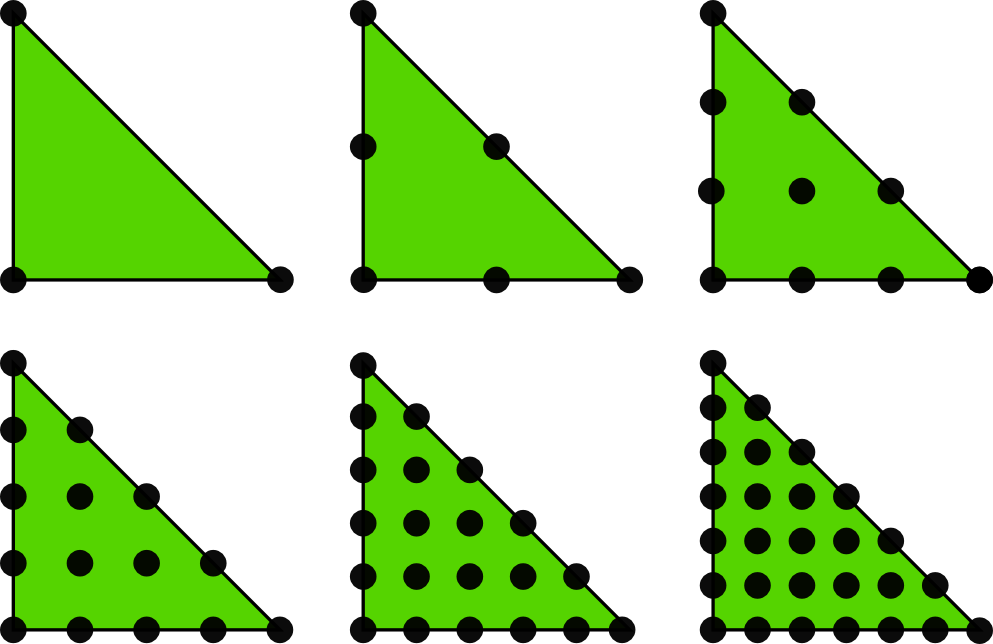
\includegraphics[width=\linewidth]{fem_triangle_2.png}
  \caption{Finite Element nodes on triangle for polynomials of different degrees, Source:http://hplgit.github.io/INF5620/doc/pub/sphinx-fem/.\_main\_fem009.html}
  \label{fig:Nodes on Triangular Element}
\end{figure}

For example, Nodal basis function of degree $D=1$ in 1 dimensional domain can be represented as (To higher dimension and higher polynomial degree, the definition can be extended similarly),

\begin{equation}
\begin{aligned}
\begin{split}
\hat{\phi_i} = \frac{x-x_{i-1}}{x_i-x_{i-1}} \quad \textrm{for} \quad x_{i-1} \leq x \leq x_i\\
\hat{\phi_i} = \frac{x_{i+1}-x}{x_{i+1}-x_{i}} \quad \textrm{for} \quad x_{i} \leq x \leq x_{i+1}\\
\end{split}
\end{aligned}
\end{equation}
\begin{center}
$\hat{\phi_i} = 0$ else
\end{center}

We do not use Nodal basis function in our analysis, instead we use orthonormal basis function.

\subsection{Orthonormal basis functions}

Orthonormal basis functions are the basis functions defined in such a way that all basis functions are orthonormal to each other with respect to suitable inner product. The number of orthonormal basis functions for a given element is the same as the number of nodal basis functions. 

\begin{equation}
\begin{split}
(\hat{\phi_i } , \hat{\phi_j}) = \int_{\hat{T}} \hat{\phi_i} \hat{\phi_j} = 1 \quad \textrm{if} \quad i = j \\
(\hat{\phi_i } , \hat{\phi_j}) = \int_{\hat{T}} \hat{\phi_i} \hat{\phi_j} = 0 \quad \textrm{if} \quad i \neq j 
\end{split}
\end{equation}

In the present analysis, $(\cdot,\cdot)$ represents $L^2$ scalar product and $\hat{T}$ is reference triangle (Section \ref{section_glob_loc}). 

\section{Global and local coordinate system} \label{section_glob_loc}

Integral terms are evaluated on a reference triangle instead of the element itself. Accordingly, a coordinate transformation between reference triangle and element is performed for evaluating integrals. The coordinate system in which the reference triangle lies is called reference or local coordinate system and the coordinate system in which element itself lies is called global coordinate system. The reference triangle has vertices $(0,0),(1,0),(0,1) \in \mathbb{R}^2$ in order. The element is defined by vertex indices in order forming triangle. The transformation from local coordinate $\hat{X}$ to global coordinate $X$ is defined by the mapping,
\begin{equation}\label{local global mapping}
F_k:\hat{X} \mapsto X \quad \forall \quad \hat{X} \in \hat{T} \quad \textrm{and} \quad X \in \mathcal{T}
\end{equation}

This mapping function is defined as,

\begin{equation}\label{local global mapping equation}
F_k(\hat{X}): X = J_k \hat{X} + C
\end{equation}

Here,
\\
$J_k$ = Jacobian matrix of element $\tau_k$ for transformation from local coordinate system to global coordinate system, $J_k \in \mathbb{R}^{d \times d}$\\
$C$ = Translational vector for transformation from local coordinate system to global coordinate system, $C \in \mathbb{R}^d$\\
$X$ = Coordinates of a point in Global coordinate system, $X \in \mathcal{T}$ \\
$\hat{X}$ = Coordinates of a point in local coordinate system, $\hat{X} \in \hat{T}$\\

We represent the image of a global function space or grid constituent on reference triangle by superscript $\hat{•}$ . This function space is known as local basis function space. 

\begin{picture}(300,100)(0,0) 
\put(0,0){\line(1,0){50}}
\put(50,0){\line(1,1){100}}
\put(0,0){\line(3,2){150}}
\put(200,0){\line(1,0){100}}
\put(300,0){\line(-1,1){100}}
\put(200,100){\line(0,-1){100}}
\end{picture}

\begin{center}
Global geometry (left) to Local geometry (right)
\end{center}

The volume integral of a function $g(x)$ in global coordinates is related to volume integral on reference geometry as 
\begin{equation}\label{integral_local_global_volume}
\int_\Omega g(x) dx = \sum_{k=1}^{nel} \int_{\tau_k} g(x) dx = \sum_{k=1}^{nel} \int_{\hat{T}} g(\hat{x}) |\det(J_k)| d \hat{x}
\end{equation}

The linear boundary integral of a function $g(x)$ on global coordinates is related to boundary integral on reference geometry as, 
\begin{equation}\label{integral_local_global_boundary}
\int_{\Gamma} g(x) ds = \int_{\hat{\Gamma}} g(\hat{x}) ld \hat{s}
\end{equation}

Also, the following holds,
\begin{equation}\label{derivative_transformation}
\nabla g = JIT_k \quad \hat{\nabla} \hat{g} 
\end{equation}


where,
\\
$l$ = length of an edge on $\mathcal{T}$\\
$g$  = A function in global coordinate system, $g:\Omega \mapsto \mathbb{R}$\\
$\hat{g}$  = A function in local coordinate system corresponding to function in $g$ in global coordinate system, $\hat{g}:\hat{T} \mapsto \mathbb{R}$\\
$JIT_k$ = $J_k^{-1}$, Jacobian inverse transpose of element $k$ \\

Here $g$ and $\hat{g}$ satisfy,
\begin{equation}\label{func_transformation}
g(x) = \hat{g}(\hat{x}) \quad \textrm{for}  \quad x = F_k(\hat{x}) \quad \textrm{according to equation \eqref{local global mapping equation}}
\end{equation}

\section{Jump operator}

The jump operator of a quantity $[u]$ at an internal boundary is defined as,
\begin{equation}\label{jump operator}
[u]=u^+ \cdot n^+ + u^- \cdot n^-
\end{equation}

where $n$ is the unit normal to an edge of an element pointing outward from the element.

As pointed out by Montlaur et al. \cite{Montlaur2} this jump representation has two disadvantages.\\

1. The function space of the quantity itself and the function space of the jump are different that is, the jump of a vector is scalar and jump of a scalar is vector.\\
2. The use of this definition camouflages the presence of a normal.\\

To overcome these disadvantages Montlaur et al. \cite{Montlaur2} modified jump representation as,\\

1.  
\begin{center}
$[pn] = p^+ n^+ + p^- n^- $ on $\Gamma$\\
$[pn] = p n $ on $\Gamma_D$\\
where $p$ is scalar.
\end{center}

2. \\
\begin{center}
$[n \otimes u] = n^+ \otimes u^+ + n^- \otimes u^-$ on $\Gamma$\\
$[n \otimes u] = n \otimes u$ on $\Gamma_D$\\
 or \\
$[n \cdot u] = n^+ \cdot u^+ + n^- \cdot u^-$ on $\Gamma$\\
$[n \cdot u] = n \cdot u$ on $\Gamma_D$\\
where $u$ is vector and $n \otimes u = u_i n_j$\\ 
\end{center}

As can be seen the quantity and its jump are now in same space i.e. jump of vector is vector and jump of scalar is scalar.

\section{Average operator}

The average operator is defined as,

\begin{equation}\label{average operator}
\left\lbrace u \right\rbrace = \frac{u^+ + u^-}{2}  
\end{equation} 

As can be seen definition of average operator does not involve normal and hence, is simpler as compared to the Jump operator.\\
Also, $u$ and $\lbrace u \rbrace$ are in same function space i.e. average of a vector is vector and average of scalar is scalar.\\

\section{$L^2$ scalar product}

We denote the scalar product of $p$ and $q$ by $(p,q)$ which refers to,\\

If $p$ and $q$ are scalars,
\begin{equation}\label{inner product scalars}
(p,q)=\int_{\Omega} pq
\end{equation}

If $p$ and $q$ are vectors,
\begin{equation}\label{Inner product vectors}
(p,q)=\int_{\Omega} p \cdot q 
\end{equation}

If $p$ and $q$ are tensors,
\begin{equation}\label{Inner product tensors}
(p,q)=\int_{\Omega} p \vdots q \quad \textrm{where} \quad p:q = Tr(pq^T)
\end{equation}

\section{Problem statement}

With the above background we are now ready to derive weak formulation and define problem in weak form. Following the approach presented by Montlaur et al. \cite{Montlaur} and Montlaur et al. \cite{Montlaur2} we arrive at the weak form of the Stokes equation and the Navier Stokes equation interior penalty approximation.

\subsection{Stokes strong, weak and discrete form} \label{Stokes_flow_ch3}

The strong form of the Stokes equation is as follow,

\begin{equation} \label{stokes_strong_form_ch3}
-\nu \Delta u + \nabla p = f \quad \textrm{in} \quad \Omega \quad \textrm{.}
\end{equation}

\begin{equation} \label{dirichlet condition stokes_ch3}
u = u_D \quad \textrm{on} \quad \Gamma_D \quad \textrm{.}
\end{equation}

\begin{equation} \label{neumann condition stokes_ch3}
-pn + \nu n \cdot \nabla u = t \quad \textrm{on} \quad \Gamma_N \quad \textrm{.}
\end{equation}


\subsubsection{Derivation of the weak form of the Stokes equation} \label{derivation_weak_stokes}

We multiply the Equation \ref{stokes_strong_form_ch3} by $\phi$ and integrate over $\mathcal{T}$,
\begin{equation}
\int_{\mathcal{T}} (- \phi \nu \Delta u + \phi \cdot \nabla p) = \int_{\mathcal{T}} \phi \cdot f 
\end{equation}

By applying Gauss divergence theoreom,
\begin{equation}
\int_{\mathcal{T}} (-\nabla (\phi \nu \nabla u) + (\nu \nabla \phi \vdots \nabla u) + \nabla \cdot (p \phi) - (p \nabla \cdot \phi)) = \int_{\mathcal{T}} \phi \cdot f 
\end{equation}

\begin{equation}
\int_{\Gamma \cup \Gamma_D \cup \Gamma_N} (- [(\phi \nu \nabla u)] + \int_{\mathcal{T}}  (\nu \nabla \phi \vdots \nabla u) + \int_{\Gamma \cup \Gamma_D \cup \Gamma_N}  [p \phi] - \int_{\mathcal{T}}  (p \nabla \cdot \phi)) = \int_{\mathcal{T}} \phi \cdot f 
\end{equation}

Following symmetric formulation for jump operator proposed by Peraire et al. \cite{peraire},
\begin{equation}
\int_{\Gamma \cup \Gamma_D \cup \Gamma_N} [(\phi \nu \nabla u)] = \int_{\Gamma} (\lbrace \phi \rbrace \vdots [n \otimes \nabla u]) + \int_{\Gamma} (\lbrace \nabla u \rbrace \vdots [n \otimes \phi]) + \int_{\Gamma_D \cup \Gamma_N} (\phi \cdot u ) 
\end{equation}

and 

\begin{equation}
\int_{\Gamma \cup \Gamma_D \cup \Gamma_N} [p \phi] = \int_{\Gamma} (\lbrace p \rbrace [ n \cdot \phi]) + \int_{\Gamma} (\lbrace \phi \rbrace \cdot [pn]) + \int_{\Gamma_D \cup \Gamma_N} (p (n \cdot \phi) ) \quad \textrm{.}
\end{equation}

It is to be notd that analytical solution is continuous and hence $[u] = 0$. Therefore we add the term $([u],[\phi])$ which helps to maintain the coercivity of discontinuous approximation.


Collecting all Neumann boundary integral terms, the weak form of Stokes equation is as follow,

\begin{equation}\label{stokes_weak_ch3}
\begin{split}
a_{IP}(u,\phi) + b(\phi,p) + (\{p\},[n\cdot \phi])_{\Gamma \cup \Gamma_D} = l_{IP}(\phi) \quad \textrm{.}
\end{split}
\end{equation}

\begin{equation}
\begin{split}
a_{IP}(u,\phi) = (\nabla u, \nabla \phi) + C_{11} ([n \otimes u],[n \otimes \phi])_{\Gamma \cup \Gamma_D} \\
- \nu (\{\nabla u\},[n \otimes \phi])_{\Gamma \cup \Gamma_D} - \nu ([n \otimes u],\{\nabla \phi\})_{\Gamma \cup \Gamma_D} \quad \textrm{.}
\end{split}
\end{equation}

It is to be noted that penalty paramter $C_{11}$ is to be kept large enough to maintain coercivity of bilinear form.

\begin{equation}
b(\phi,\psi) = -\int_{\mathcal{T}} \psi \nabla \cdot \phi
\end{equation}

\begin{equation}
\begin{split}
l_{IP}(\phi) = (f,\phi) + (t,\phi)_{\Gamma_N} + C_{11} (u_D,\phi)_{\Gamma_D} - (n \otimes u_D, \nu \nabla \phi)_{\Gamma_D}
\end{split}
\end{equation}

The discrete form of Stokes equation is written as,

\begin{equation} \label{stokes discrete_ch3}
AU + BP = F_1 \quad \textrm{.}
\end{equation}

Matrix $A$ and matrix $B$ are calculated as per equation \ref{matrix A} and equation \ref{matrix B} respectively. \\

The strong form of continuity equation is as follow,

\begin{equation}
\nabla \cdot u = 0 \quad \textrm{in} \quad \Omega \quad \textrm{.}
\end{equation}

and the weak for of continuity equation is as follow,

\begin{equation}\label{contiuity_weak_ch3}
\begin{split}
b(u,\psi) + (\{\psi\},[n\cdot u])_{\Gamma \cup \Gamma_D} = (q,n\cdot u_D)_{\Gamma_D} \quad \textrm{.}
\end{split}
\end{equation}

The discrete form of continuity equation is written as,

\begin{equation} \label{continuity discrete_ch3}
B^T U  = F_2 \quad \textrm{.}
\end{equation}

Discrete form of equations can be written in Matrix form as, 

\begin{equation} \label{Stokes_matrix_ch3}
\begin{spmatrix}{\textrm{Stiffness matrix}}
    A & B \\
    B^T & 0
\end{spmatrix}
\begin{spmatrix}{\textrm{Solution vector}}
    U \\
    P
\end{spmatrix}
=
\begin{spmatrix}{\textrm{Right hand side (Known)}}
    F_1  \\
    F_2
\end{spmatrix}
\end{equation}

Here, $(\cdot , \cdot)$ is $L^2$ inner product, $\{\cdot\}$ is average operator, $[\cdot]$ is jump operator. 

\subsection{Properties of the stiffness matrix} \label{property_stif_mat_stokes}

We now write each element of matrix $A$. We represent components of Unit normal vector as $n = [n_1 \quad ... \quad n_d]$

\begin{equation} \label{matrix A}
\begin{split}
A_{ij} = \sum_{k=1}^d (\frac{\partial \phi_i}{\partial x_k} , \frac{\partial \phi_j}{\partial x_k}) + C_{11} \sum_{k=1}^d ([\phi_i n_k] , [\phi_j n_k])_{\Gamma \cup \Gamma_D} \\ - \nu \sum_{k=1}^d ([\phi_i n_k] , \lbrace \frac{\partial \phi_j}{\partial x_k} \rbrace)_{\Gamma \cup \Gamma_D} - \nu \sum_{k=1}^d (\lbrace \frac{\partial \phi_i}{\partial x_k} \rbrace , [\phi_j n_k])_{\Gamma \cup \Gamma_D}
\end{split}
\end{equation}

We can see following properties of $A$: 
\\
1. $A_{ij} = A_{ji} \implies$ Symmetric\\
2. $A$ is positive definite : As the penalty parameter $C_{11}$ is adjusted to ensure coercivity of $A$ (Section \ref{Coercivity_constant}),\\
$\exists \quad c' > 0 $ and for non zero vector $z$
\begin{equation}
z^T A( \phi , \phi ) z \geq c' || z ||^2 \implies z^T A( \phi , \phi ) z > 0
\end{equation}
3. Size of matrix $A$: $A \in \mathbb{R}^{u_{ndofs} \times u_{ndofs}}$ ($u_{ndofs}$ is total number of degrees of freedom of velocity)\\

Each element of $B$ can be represented as,\\
\begin{equation} \label{matrix B}
B_{ij} = - \int_\mathcal{T} \frac{\partial \phi_i}{\partial x_i} \psi_j + (\lbrace \psi_j \rbrace , [n \cdot \phi_i])_{\Gamma \cup \Gamma_D}
\end{equation}

We notice that, Size of matrix $B$: $B \in \mathbb{R}^{u_{ndofs} \times p_{ndofs}}$ ($p_{ndofs}$ is total number of degrees of freedom of pressure)

$u_{ndofs}$ and $p_{ndofs}$ on triangular grid and taylor-hood pressure velocity basis function can be calculated as below. In present analysis we have $d_u = 2$ and $d_p = 1$.

\begin{equation} \label{undofs}
u_{ndofs} = 2 \quad \left( \frac{(D+1)(D+2)}{2} \right) \quad nel
\end{equation}

\begin{equation} \label{pndofs}
p_{ndofs} = \left(\frac{D(D+1)}{2}\right) \quad nel
\end{equation}

With above considerations we arrive at following conclusions, \\

1. Stiffness matrix is symmertic. \\
2. Stiffness matrix $ \in \mathbb{R}^{(u_{ndofs} + p_{ndofs}) \times (u_{ndofs} + p_{ndofs})}$\\
3. The number of positive eigenvalues of stiffness matrix is equal to number of velocity degrees of freedom and number of negative eigenvalues of stiffness matrix is equal to number of pressure degrees of freedom.\\

\subsubsection{Proof}

From equation \eqref{factorisation1} we see that the congruent matrix of the stiffness matrix for Stokes equation is,
\begin{equation}
\begin{spmatrix}{}
    A & 0 \\
    0 & S
\end{spmatrix}
\end{equation}
We look at the the eigenvalues of $S$ as the number of positive and negative eigenvalues of congruent matrix and stiffness matrix are same.\\
We see that $S \in \mathbb{R}^{p_{ndofs} \times p_{ndofs}}$, $S = - B^T A^{-1} B$.\\ 
For any non zero vector $z$, $z^T S z < 0$ i.e. $S$ is symmetric negative definite and hence, all eigenvalues of $S$ are negative.

\subsubsection{Coercivity constant for equation for Stokes flow} \label{basics}

We define a lower and upper bound for the kinematic viscosity such that \\
\begin{equation}
\nu_0 \leq \nu \leq \nu_1
\end{equation}

Using Cauchy Schwarz inequality, 

\begin{equation}
\begin{split}
\sum_{e \in \Gamma \cup \Gamma_D} \int_e {\nu}[n \otimes \phi] \leq \sum_{e \in \Gamma \cup \Gamma_D} ||\nu \nabla \phi \cdot n||_{L^2(e)} \quad ||[\phi]||_{L^2(e)} \\ \leq \sum_{e \in \Gamma \cup \Gamma_D} ||\nu \nabla \phi \cdot n||_{L^2(e)} (\frac{1}{l})^{(1/2-1/2)} \quad ||[\phi]||_{L^2(e)} \quad \textrm{.}
\end{split}
\end{equation}

Based on the Trace inequatlity and the lower and upper bound for viscocity, for neighbouring elements $\tau_{k_1}$ and $\tau_{k_2}$ sharing the edge $e$, 

\begin{equation}
\begin{split}
||\lbrace \nu \nabla \phi \cdot n \rbrace||_{L^2(e)} \leq \frac{C_t \nu_1}{2} {h_{\tau_{k_1}}^{-1/2}} ||\nabla \phi||_{L^2({\tau_{k_1}})} \\ + \frac{C_t \nu_1}{2} {h_{{\tau_{k_2}}}^{-1/2}} ||\nabla \phi||_{L^2({\tau_{k_2}})} \quad \textrm{.}
\end{split}
\end{equation}

Again based on the trace inequality, for $e \in \Gamma \cup \Gamma_D$

\begin{equation}
\begin{split}
\int_e \lbrace \nu \nabla \phi \rbrace [n \otimes \phi] \leq \frac{C_t \nu_1}{2}  \left( h_{(\tau_{k_1})}^{\frac{-1}{2}} ||\nabla \phi||_{L^2{(\tau_{k_1})}} + {h_{(\tau_{k_2})}^{\frac{-1}{2}}} ||\nabla \phi||_{L^2{(\tau_{k_2})}} \right) \\ l^{\frac{\beta_0}{2}} \left({\frac{1}{l}}\right)^{\frac{\beta_0}{2}} ||[\phi]||_{L^2(e)} \quad \textrm{.}
\end{split}
\end{equation}

For $h_{\tau_k} \leq 1$ and the $\beta_0 (d-1) \geq 1$ we obtain a similar bound for the boundary edges.

If $n_0$ denotes maximum number of neighbours ($n_0 = 3$ for triangles),
\begin{equation}
\begin{split}
\int_e \lbrace \nu \nabla \phi \rbrace[n \otimes \phi] \leq C_t \nu_1 \left( \sum_{e \in \Gamma_h \cup \Gamma_D} \frac{1}{l^\beta_0} ||[\phi]||^2_{L^2(e)} \right)^{1/2} \\ \times \left( \sum_{e \epsilon \Gamma_h} ||\nabla \phi||^2_{L^2(\tau_{k_1})} + ||\nabla \phi||^2_{L^2(\tau_{k_2})} + \sum_{e \epsilon \Gamma_D} ||\nabla \phi||^2_{0,\tau_{k_1}} \right)
\end{split}
\end{equation}

\begin{equation}
\begin{split}
\int_e \lbrace \nu \nabla \phi \rbrace[n \otimes \phi] \leq C_t \nu_1 \sqrt{n_0} \left( \sum_{e \in \Gamma_h \cup \Gamma_D} \frac{1}{l^\beta_0} ||[\phi]||^2_{L^2(e)} \right)^{1/2} \\ \left( \sum_{e \in \Gamma_h \cup \Gamma_D} ||\nabla \phi||^2_{L^2(\tau)} \right) \quad \textrm{.}
\end{split}
\end{equation}

Using Young's inequality for $\delta > 0$

\begin{equation}
\sum_{e \in \Gamma \cup \Gamma_D} \int_e \lbrace \nu \nabla \phi \rbrace [n \otimes \phi] \leq \frac{\delta}{2} \sum_{\tau \in \mathcal{T}} ||\nu^{1/2} \nabla \phi ||^2_{L^2(\tau)} +  \frac{C_t^2 \nu_1^2 n_0}{2 \delta \nu_0}  \sum_{e \in \Gamma \cup \Gamma_D} \frac{1}{l^{\beta_0}} ||[\phi]||^2_{L^2(e)}
\end{equation}


\begin{equation}
a_\epsilon (\phi , \phi) \geq \left( 1-\frac{\delta}{2} |1-\epsilon| \right) \sum_{\tau \epsilon \mathcal{T}} ||\nu^{1/2} \nabla v ||^2_{L^2(\tau)} + \sum_{e \epsilon \Gamma_h \cup \Gamma_D} \frac{\sigma_e^0 - \frac{C_t^2 \nu_1^2 n_0}{2 \delta K_0}|1-\epsilon|}{l^{\beta_0}} ||[v]||^2_{L^2(e)}
\end{equation}

where, we have penalty parameter,
\begin{equation}
C_{11} = \frac{\kappa_e}{l}
\end{equation} 

where, $\kappa_e$ is coercivity constant.

We can obtain exact expression for $\kappa_e$ for triangular mesh and Symmetric Interior Penalty Galerkin formulation $\epsilon = -1$ as,\\
\begin{equation}
\begin{split}
\kappa_e = \frac{3 ( {\nu_1}^{\tau_{k_1}})^2}{2 {\nu_0}^{\tau_{k_1}}} D (D+1) l^{\beta_0 - 1} cot {\theta^{\tau_{k_1}}}  \\ + \frac{3 ( {\nu_1}^{\tau_{k_2}})^2}{2 {\nu_0}^{\tau_{k_2}}} D (D+1) l^{\beta_0 - 1} cot {\theta^{\tau_{k_2}}}
\end{split}
\end{equation} 

\subsection{Upwinding} \label{upwinding}

Upwinding is the method used to discretise the convective term. In the case of Discontinuous Galerkin method we define the upwinding as follow.\\

If $n_\tau$ is the unit normal from $\tau_1$ to $\tau_2$ and if we denote the upwind value of function $g$ as $g^{up}$ \cite{riviere},
\begin{equation}
\begin{split}
g^{up} = g|_{\tau_1} \quad \textrm{if} \quad g \cdot n_\tau \geq 0 \\
g^{up} = g|_{\tau_2} \quad \textrm{if} \quad g \cdot n_\tau < 0
\end{split}
\end{equation}
\\
In our analysis this is explicitly defined in the term $c(u,u,\phi)$ in section \ref{n_s_ch3}. The formulation is such that,
\begin{equation}
\begin{split}
u^{up} = u \quad \textrm{if} \quad u \cdot n \geq 0 \\
u^{up} = u^{ext} \quad \textrm{if} \quad u \cdot n < 0
\end{split}
\end{equation}

\subsection{Navier Stokes strong, weak and discrete form} \label{n_s_ch3}

Stokes flow is an example of the Navier Stokes flow with low Reynolds number, $Re$. In case of high Reynolds number the inertial force can no longer be neglected and hence we need to add inertial forces in Stokes flow. 

The strong form of the Navier Stokes equation can be written as,

\begin{equation} \label{navier_stokes_strong_ch3}
-\nu \Delta u + \nabla p + (u \cdot \nabla) u = f \quad \textrm{in} \quad \Omega \quad \textrm{.}
\end{equation}

with Dirichlet and Neumann boundary condition as per section \ref{Stokes_flow_ch3}. Also the continuity equation as mentioned in section \ref{Stokes_flow_ch3} is valid.

The inertial forces term i.e. $(u \cdot \nabla) u$ in weak form with upwinding (section \ref{upwinding}) is represented as below,

\begin{equation}
\begin{split}
c(g;u,\phi) = \sum_{i=1}^{nel} \int_{\partial \Omega_i \setminus \Gamma_N} \frac{1}{2} [[(g \cdot n_i)(u^{ext} + u) - |g \cdot n_i|(u^{ext} - u)]] \cdot \phi \\ + \int_{\Gamma_N} (g\cdot n) u \cdot \phi -((g\cdot \nabla)\phi,u)
\end{split}
\end{equation}

\begin{equation} \label{uext}
u^{ext} = \lim_{\epsilon \rightarrow 0} u(x+\epsilon n_i) \quad  \textrm{for} \quad x \in \partial \mathcal{T}_i
\end{equation}

Hence, the Navier Stokes equation can be written as,

\begin{equation}\label{navier_stokes_weak_ch3}
\begin{split}
a_{IP}(u,\phi) + c(u;u,\phi) + b(\phi,p) + (\{p\},[n\cdot \phi])_{\Gamma \cup \Gamma_D} = l_{IP}(\phi) 
\end{split}
\end{equation}

Here, we can see that the $c(u,u,\phi)$ is non linear term.

In discrete form this equation can be written as,

\begin{equation}
AU + C(U) U + BP = F
\end{equation} 

Here, $C(U)$ is a matrix which is dependent on solution vector $U$ and hence making the system of equation non linear.

In matrix form the Navier Stokes equation with continuity equation can be written as,

\begin{equation} \label{navier_Stokes_matrix_ch3}
\begin{spmatrix}{\textrm{Stiffness matrix}}
    A+C(U) & B \\
    B^T & 0
\end{spmatrix}
\begin{spmatrix}{\textrm{Solution vector}}
    U \\
    P
\end{spmatrix}
=
\begin{spmatrix}{{\textrm{Right hand side (Known)}}}
    F_1  \\
    F_2
\end{spmatrix}
\end{equation}

In the present analysis, we use Newton method to solve nonlinear system of equations. We present the Newton scheme in section \ref{newton_method}. 

Our problem statement now reduces to, find $(u,p) \in (\mathbb{V},\mathbb{Q})$ such that $\forall (\phi,\psi) \in (\mathbb{V},\mathbb{Q})$ equation \ref{stokes_weak_ch3} for the Stokes flow and equation \ref{navier_stokes_weak_ch3} for the Navier Stokes flow is satisfied.

\subsection{Newton method} \label{newton_method}

We derive Newton method as per method presented by Haasdonk B. \cite{Haasdonk} for solving nonlinear system of equations arising out of the discrete form of the Navier Stokes equation. For $u, \phi , h \in \mathbb{V}$ and $p, \psi , h' \in \mathbb{Q}$ \\
\begin{flushleft}
\begin{equation}
S(u) = a(u,\phi) + b(\phi,p) + (\{p\},[n\cdot \phi])_{\Gamma \cup \Gamma_D} - l_{IP}(\phi)
\end{equation}
\end{flushleft}

\begin{flushleft}
\begin{equation}
\begin{split}
S(u+h) - S(u) = (a(u+\delta h,\phi) + c(u + \delta h;u + \delta h,\phi)\\ + b(\phi,p+\delta h') + (\{p+\delta h'\},[n\cdot \phi])_{\Gamma \cup \Gamma_D} - l_{IP}(\phi)) - (a(u,\phi)\\ + c(u,u,\phi) + b(\phi,p) + (\{p\},[n\cdot \phi])_{\Gamma \cup \Gamma_D} - l_{IP}(\phi))
\end{split}
\end{equation}
\end{flushleft}

\begin{flushleft}
\begin{equation}
\begin{split}
S(u+h) - S(u) = 2\delta c(u,h,\cdot) + \delta^2 c(h,h,\cdot) + \delta a(h,\cdot)\\ + \delta b(h',\cdot) + \delta (\{h'\},[n\cdot \phi])_{\Gamma \cup \Gamma_D}
\end{split}
\end{equation}
\end{flushleft}

\begin{flushleft}
\begin{equation}
DS(u) = \lim_{\delta \to 0} \frac{S(u+h)-S(u)}{\delta}
\end{equation}
\end{flushleft}

\begin{flushleft}
\begin{equation}
\begin{split}
DS(u) = 2 c(u,h,\cdot) + a(h,\cdot) + b(h',\cdot) + (\{h'\},[n\cdot \phi])_{\Gamma \cup \Gamma_D}
\end{split}
\end{equation}
\end{flushleft}

Following similar procedure we write for continuity equation:\\
\begin{flushleft}
\begin{equation}
S'(u) = b(u,\psi) + (\{\psi\},[n \cdot u])_{\Gamma \cup \Gamma_D} - (\psi,n \cdot u_D)_{\Gamma_D}
\end{equation}
\end{flushleft}

\begin{flushleft}
\begin{equation}
S'(u+\delta h) = b(u + \delta h,\psi) + (\{\psi\},[n \cdot u + \delta h])_{\Gamma \cup \Gamma_D} - (\psi,n \cdot u_D)_{\Gamma_D}
\end{equation}
\end{flushleft}

\begin{flushleft}
\begin{equation}
DS'(u) = b(\delta h,\psi) + (\{\psi\},[n \cdot \delta h])_{\Gamma \cup \Gamma_D} 
\end{equation}
\end{flushleft}


Algotrithm for the Newton method is as follow:\\

1. Select $u^{iter} \in \mathbb{V}$ at iteration $iter$\\

2. Verify $DS_{u^{iter}}(h^{iter}) = -S(u^{iter})$\\

3. Set $u^{iter + 1} := u^{iter} + h^{iter}$ till $||u^{iter+1} - u^{iter}|| < tol$ where $tol$ is specified tolerance.\\

In discrete form the Newton method means, solving the equation (at iteration = $iter$)

\begin{flushleft}
\begin{equation}
\begin{spmatrix}{\textrm{Stiffness matrix}^{iter}}
    A+C(U^{iter}) & B \\
    B^T & 0
\end{spmatrix}
\begin{spmatrix}{\textrm{Solution vector}^{iter+1}}
    U^{iter+1} \\
    P^{iter+1}
\end{spmatrix}
=
\begin{spmatrix}{\textrm{Right hand side (Known function)}}
    F_1  \\
    F_2
\end{spmatrix}
\end{equation}
\end{flushleft}

to reach convergence i.e. $||U^{iter+1} - U^{iter}|| < tol$, some specified tolerance.\\

For success of the Newton method it is important to have good initial guess. For the Newton method we use solution of the Stokes equation as initial guess.

\subsection{Properties of the stiffness matrix} \label{property_stif_mat_navier}

Each element of $C$ can be represented as,\\

at newton iteration $iter + 1$,
\begin{flushleft}
\begin{equation} \label{matric C}
\begin{split}
C_{IJ} = \sum_{i=1}^{nel} \int_{\partial \mathcal{T}_i \setminus \Gamma_N} \frac{1}{2} [[(U^{iter} \cdot n_i)({\phi^{ext}}_J + {\phi}_J ) - |U^{iter} \cdot n_i|({{\phi}^{ext}}_J - {\phi}_J)]] \cdot \phi_I \\ + \int_{\Gamma_N} (U^{iter} \cdot n) \phi_J \cdot \phi_I -((U^{iter} \cdot \nabla)\phi_J,\phi_I)
\end{split}
\end{equation}
\end{flushleft}

Size of matrix : $C \in \mathbb{R}^{u_{ndofs} \times u_{ndofs}}$. \\

We now can see that whereas the stiffness matrix of the Stokes equation is symmetric and has Symmetric positive definite part $A$, the stiffness matrix of the Navier Stokes equation is non symmetric.

\subsection{Boundary conditions}

We impose in our analysis boundary conditions weakly. This is done by the linear terms on right hand side of equation  $(t,\phi)_{\Gamma_N}$, $(u_D,\phi)_{\Gamma_D}$, \linebreak $(n \otimes u_D, \nu \nabla \phi)_{\Gamma_D}$ in equation \ref{navier_stokes_weak_ch3} and equation \ref{stokes_weak_ch3}.

\section{Selection of solver}

In order to solve the variation form of the Stokes equation we use Biconjugate gradients stabilized method popularly known as $bicgstab$, Minimum residual method better known as $minres$ and Schur complement method. The $bicgstab$ and $minres$ are in built solvers of MATLAB. Schur complement method (Section \ref{schur}) is implemented separately based on Cholesky decomposition (Section \ref{chol}).

\subsection{Biconjugate gradients stabilized method}

The $bicgstab$ works to minimise residual of linear equation of the form:

\begin{equation} \label{linear_matrix_equation}
KX = B
\end{equation}

with $K$ = Coefficient matrix, $X$ = Vector of unknowns and $B$ = vector of value of known function. The coefficient matrix $A$ need not be symmetric. We refer to \cite{bicgstab} for details about the method.\\

\subsection{Minimum residual method} 

The $minres$ method is a special kind of conjugate gradient method but does not require LU decomposition. We refer to \cite{minres} for details about the method. It also solves the equations \ref{linear_matrix_equation}. However, the coefficient matrix $K$ must be symmetric. \\

As the coefficient matrix in case discrete form of Stokes equation is symmetric, the $minres$ is suitable solver. Moreover, it has shown to coverge to required convergence level, provided sufficient number of iterations, when $bicgstab$ is not able to reach required level of convergence.

\subsection{Schur complement method} \label{schur}

We subdivide the matrix form of the Stokes equation \eqref{Stokes_matrix} into smaller dimension system by Schur complement method. We also note that matrix $A$ is symmetric positive definite and matrix $K$ is symmetric.
Here, $A \in \mathbb{R}^{u_{ndofs} \times p_{ndofs}}$; $B \in \mathbb{R}^{u_{ndofs} \times p_{ndofs}}$; $U,F_1 \in \mathbb{R}^{u_{ndofs}}$; $P, F_2 \in \mathbb{R}^{p_{ndofs}}$. \\

We solve equation \eqref{Stokes_matrix} in following steps,\\

STEP 1: \\ 
\begin{equation}\label{schur step 1}
U = A^{-1}(F_1 - BP) 
\end{equation}

The matrix $A$ is inverted by Cholesky decomposition (section \ref{chol}). 

STEP 2 : \\
We substitute now equation \eqref{schur step 1} into equation \eqref{continuity discrete_ch3} and \eqref{stokes discrete_ch3}
\begin{equation}\label{schur step 2}
- B^T A^{-1} B P = F_2 - B^T A^{-1} F_1
\end{equation}

STEP 3 : \\
We now back substitute $P$ in equation \eqref{schur step 1} and compute $U$ in order to eventually obtain the solution vector.
\\

As pointed by Fritzen F. \cite{Fritzen}, the success of this method primarily depends upon the sparsity pattern of $B$ and efforts required for inverting $A$. The Cholesky decomposition provides faster approach for inverting $A$ due to symmetric positive definite nature of $A$. \\

In the present analysis, we find that the Schur complement method is much faster and in fact, for low flow velocities accurate method. Also Cholesky decomposition provides error message in case $A$ is not symmetric positive definite, indicating improper choice of penalty parameter. 

\chapter{Implementation aspects} \label{implementation_aspects}

We discuss now the implementation of the discrete formulation of the Navier Stokes discontinuous Galerkin weak formulation in RBmatlab, A MATLAB library containing all our numerical simulation approaches for linear and nonlinear, affine or arbitrarily parameter dependent evolution problems with finite element, finite volume or local discontinuous Galerkin discretizations. We refer to the literature of Haasdonk B.\cite{Haasdonk_book} and RBmatlab website: \\
http://www.ians.uni-stuttgart.de/MoRePaS/software/rbmatlab/1.16.09/\linebreak index.html.  

Before we discuss details of the implementation it is important to understand some frequently used terminologies and the data type of Basis Function and derivative of basis function in RBmatlab.

\section{Terminology}

A. \verb|params| and \verb|paramsP| : These are structures corresponding to velocity and pressure respectively and primarily containing following fields. (Table \ref{table_params} and Table \ref{table_paramsP})\\

B. \verb|grid| : It is the structure containing fields relevant to information stored in grid. (Table \ref{table_grid})\\

C. We also define some other variables. (Table \ref{table_variable})\\

\begin{table}
\cprotect\caption{Fields of \verb|params|}
\label{table_params}
\begin{center}
\begin{tabular}{| p{.25\textwidth}| p{.25\textwidth} |  p{.25\textwidth} | p{.25\textwidth}|} 
\hline
\textbf{Fieldname} & \textbf{Representation} & \textbf{Size} & \textbf{Description}\\
\hline
\verb|dimrange| & $d_u$ & $\mathbb{N}$ & User defined field\\
\hline
\verb|pdeg| & $D$ & $\mathbb{N}$ & User defined field\\
\hline
\verb|ndofs_per_element| & $u_{npe}$ & $\mathbb{N}$ & Calculated as per equation \ref{unpe}\\
\hline
\verb|ndofs| & $u_{ndofs}$ & $\mathbb{N}$ & Calculated as per equation \ref{undofs}\\
\hline
\verb|dofs| & $U$ & $\mathbb{R}^{u_{ndofs}}$ & Calculated after solving \ref{navier_stokes_weak_ch3} and \ref{stokes_weak_ch3}\\
\hline
\verb|show_sparsity| & - & Bool variable & User defined switch to plot sparsity pattern\\
\hline
\end{tabular}
\end{center}
\end{table}

\begin{table}
\cprotect\caption{Fields of \verb|paramsP|}
\label{table_paramsP}
\begin{center}
\begin{tabular}{| p{.25\textwidth}| p{.25\textwidth} |  p{.25\textwidth} | p{.25\textwidth}|}
\hline
\textbf{Fieldname} & \textbf{Representation} & \textbf{Size} & \textbf{Description}\\
\hline
\verb|dimrange| & $d_p$ & $\mathbb{N}$ & User defined field\\
\hline
\verb|pdeg| & $D-1$ & $\mathbb{N}$ & Calculated as taylor hood element\\
\hline
\verb|ndofs_per_element| & $p_{npe}$ & $\mathbb{N}$ & Calculated as per equation \ref{pnpe}\\
\hline
\verb|ndofs| & $p_{ndofs}$ & $\mathbb{N}$ & Calculated as per equation \ref{pndofs}\\
\hline
\verb|dofs| & $P$ & $\mathbb{R}^{p_{ndofs}}$ & Calculated after solving \ref{navier_stokes_weak_ch3} and \ref{stokes_weak_ch3}\\
\hline
\verb|show_sparsity| & - & Bool variable & User defined switch to plot sparsity pattern\\
\hline
\end{tabular}
\end{center}
\end{table}

\begin{table}
\cprotect\caption{Fields of \verb|grid|}
\label{table_grid}
\begin{center}
\begin{tabular}{| p{.25\textwidth}| p{.25\textwidth} |  p{.25\textwidth} | p{.25\textwidth}|}
\hline
\textbf{Fieldname} & \textbf{Representation} & \textbf{Size} & \textbf{Description}\\
\hline
\verb|nelement| & $nel$ & $\mathbb{N}$ & User defined or generated field\\
\hline
\verb|NBI| & $-$ & $\mathbb{R}^{nel \times n_0}$ & $NBI(i,j)$ is the $j^{\textrm{th}}$ neighbour of element $i$\\
\hline
\verb|NX| & $n_x$ & $\mathbb{R}^{nel \times d}$ & $x-$component of unit normal vector\\
\hline
\verb|NY| & $n_y$ & $\mathbb{R}^{nel \times d}$ & $y-$component of unit normal vector\\
\hline
\verb|A| & $Ar$ & $\mathbb{R}^{nel}$ & Area of element\\
\hline
\verb|EL| & $l$ & $\mathbb{R}^{nel \times n_0}$ & edge length\\
\hline
\verb|JIT| & $JIT$ & $\mathbb{R}^{nel \times n_0 \times d}$ & Jacobian inverse transpose\\
\hline
\end{tabular}
\end{center}
\end{table}

\begin{table}
\caption{Some other variables}
\label{table_variable}
\begin{center}
\begin{tabular}{| p{.25\textwidth}| p{.25\textwidth} |  p{.25\textwidth} | p{.25\textwidth}|}
\hline
\textbf{Name} & \textbf{Representation} & \textbf{Size} & \textbf{Description}\\
\hline
\verb|k| & $k$ & $\mathbb{N}$ & element number, $1 \leq k \leq nel$\\
\hline
\verb|ids| & $-$ & $\mathbb{R}^{npe}$ & indices of degrees of freedom in global vector\\
\hline
\end{tabular}
\end{center}
\end{table}

\section{Basis functions in RBmatlab}

\verb|ldg_evaluate_basis| routine of RBmatlab evaluates the basis functions at a given point.\\

We approximate the solution at any point from solution of degrees of freedom in orthonormal basis. In matrix formulation this means basis function is matrix of the size,

\begin{equation}\label{basis_func_velocity_rbmatlab}
\phi \in \mathbb{R}^{u_{npe} \times d_u}
\end{equation}

and

\begin{equation}\label{basis_func_pressure_rbmatlab}
\psi \in \mathbb{R}^{p_{npe} \times d_p} \quad \textrm{.}
\end{equation}

This representation creates many zeros in matrix, however, it does not require new evaluation for each component of vector quantity. Due to the zeros in the basis function, derivative of basis functions also has many zeros.\\

\verb|ldg_evaluate_basis_derivative| is the routine which evaluates the derivative of the basis functions. The derivative of basis function $(\phi)_{i}$, where $1 \leq i \leq u_{npe}$ is a cell containing matrix $\nabla (\phi)_{i}$ of size,

\begin{equation}\label{basis_func_derivative_velocity_rbmatlab}
\nabla (\phi)_{i} \in \mathbb{R}^{{d_u} \times d} \quad \textrm{.}
\end{equation}

The columns of the matrix correspond to $\nabla_x (\phi)_{i}$ and $\nabla_y (\phi)_{i}$.

The derivative of basis function $(\psi)_{i}$, where $1 \leq i \leq p_{npe}$ is a cell containing matrix $\nabla (\psi)_{i}$ of size,

\begin{equation}\label{basis_func_derivative_pressure_rbmatlab}
\nabla (\psi)_{i} \in \mathbb{R}^{{d_p} \times d} \quad \textrm{.}
\end{equation}

The columns of the matrix correspond to $\nabla_x (\psi)_{i}$ and $\nabla_y (\psi)_{i}$.

\section{Assembly of average operator}

Average of quantity $A_h$ in discrete form is assembled as,

\begin{equation}\label{Average operator}
\lbrace A_h \rbrace = (A_h^+ + A_h^-)/2
\end{equation}

The assembly of the average operator is relatively simple as compared to the jump operator which is explained in Section \ref{Average operator}.

\section{Assembly of jump operator} \label{Jump operator}

The jump of the quantity $A_h$ in discrete form is assembled as,
\begin{equation} \label{Jump_operator}
[A_h] = A_h^+ n^+ + A_h^- n^-
\end{equation}

In case of terms such as $[A_h],[B_h]$ we assemble matrices as, 

For internal edges $\Gamma$,

\begin{equation} \label{Jump operator L2}
[A_h],[B_h] = A_h^+ n^+ B_h^+ n^+ + A_h^+ n^+ B_h^- n^- + A_h^- n^- B_h^+ n^+ + A_h^- n^- B_h^- n^-
\end{equation}

and for Dirichlet edges $\Gamma_D$

\begin{equation} \label{Jump operator L2 for dirichlet}
[A_h],[B_h] = A_h^+ n^+ B_h^+ n^+ 
\end{equation}


\section{Matrix assemblies} \label{matrix_assembly_ch4}

It is to be noted that $\hat{\phi}$ is evaluated at local coordinate corresponding to global coordinate in accordance with the equation \ref{func_transformation}.

The matrices from weak form of Navier Stokes equation have been assembled in 3 steps,

1. Evaluating function at vertex of local element and transform to global geometry. (Equation \ref{func_transformation})\\
2. Transform function evaluation from step 1 to global geometry (if not done in step 1) and performing integral of function over local element.(Equation \ref{integral_local_global_boundary} and \ref{derivative_transformation})\\
3. Performing a loop over all elements and allocate integral at position in global matrix (for bilinear terms)/global vector (for linear terms) according to indices of element degrees of freedom in global degree of freedom vector.\\

We also perform numerical integration over domain $\Omega$ as,

\begin{equation}\label{numerical integration}
\int_{\Omega} f(x) = \sum_{i=1}^{nop} f(x_i) w_i
\end{equation}

Where, \\

$x_i$ = Location of function evaluation\\
$w_i$ = Weight at corresponding point\\
$nop$ = Number of points\\

The location of function evaluation, number of points and weights are based on Gaussian quadrature rule.

Also the determinant of the Jacobian is twice the area of triangle.

\begin{equation}\label{determinant to area}
\det J(k) = 2Ar(k)
\end{equation}

With this preliminary informations we discuss now the assembly of matrices.

\subsection{$(\nabla \phi, \nabla \phi)$}

\subsubsection{Step 1: Function evaluation}

Through \verb|ldg_evaluate_basis_derivative| and \verb|grid| structure, we first evaluate the derivative of $\hat{\phi}$ and $JIT(k,:,:)$ at point $x_i$ . We also perform elementary operation so as to receive one global basis function in each row. The matrix transformation from local derivative to global derivative is based on the equation \ref{derivative_transformation}.

We than assemble the matrix,
 
\begin{equation}
res_1[i,j]= {\nabla \phi_i} {\nabla \phi_j}^T \quad \textrm{for} \quad 1 \leq i,j \leq u_{npe} \quad \textrm{.}
\end{equation}

\subsubsection{Step 2: Performing integration in global coordinate system}

We perform the numerical integration as per equation \eqref{numerical integration} 
\begin{equation}
res_2 = \int_{\hat{T}} (res_1) (2 Ar(k))
\end{equation}

\subsubsection{Step 3: Degrees of freedom allocation in global matrix}
 
Looping over each element and performing following operation in each loop,
\begin{equation}
res_3[ids\_velocity,ids\_velocity]=res_2 \quad \textrm{.}
\end{equation}


\subsection{$([n \otimes \phi], [n \otimes \phi])_{\Gamma \cup \Gamma_D}$}

\subsubsection{Step 1: Function evaluation} 

Following matrices are evaluated in first step.

\begin{equation}
\begin{split}
res_1^{++} = (n \otimes \hat{\phi})^+ (n \otimes \hat{\phi})^+\\
res_1^{+-} = (n \otimes \hat{\phi})^+ (n \otimes \hat{\phi})^-\\
res_1^{-+} = (n \otimes \hat{\phi})^- (n \otimes \hat{\phi})^+\\
res_1^{--} = (n \otimes \hat{\phi})^- (n \otimes \hat{\phi})^-\\
\end{split}
\end{equation}

Please note that $\hat{\phi_h}$ is evaluated at local coordinate corressponding to global coordinate.

\subsubsection{Step 2: In step 2 we perform following integration}
 
We perform the numerical integration as per equation \ref{integral_local_global_boundary}.
\begin{equation}
\begin{split}
res_2^{++} = \int_{\Gamma} res_1^{++} EL(i,j)\\
res_2^{+-} = \int_{\Gamma} res_1^{+-} EL(i,j)\\
res_2^{-+} = \int_{\Gamma} res_1^{-+} EL(i,j)\\
res_2^{--} = \int_{\Gamma} res_1^{--} EL(i,j)\\
\end{split}
\end{equation}

\subsubsection{Step 3: Degrees of freedom allocation in global matrix}

Loop over all elements, define the global assembly matrix as zero matrix and perform following operation in each loop.
\begin{equation}
\begin{split}
res_3^{++}[ids\_velocity\_self,ids\_velocity\_self] = res_2^{++}\\
res_3^{+-}[ids\_velocity\_self,ids\_velocity\_neighbour] = res_2^{+-}\\
res_3^{-+}[ids\_velocity\_neighbour,ids\_velocity\_self] = res_2^{-+}\\
res_3^{--}[ids\_velocity\_neighbour,ids\_velocity\_neighbour] = res_2^{--}\\
\end{split}
\end{equation}
Finally,
\begin{equation}
res_3 = res_3^{++} + res_3^{+-} + res_3^{-+} + res_3^{--} \quad \textrm{.}
\end{equation}

It is to be noted that on dirichlet boundary only $res_1^{++}, res_2^{++}, res_3^{++}$ is evaluated as all other terms are zero.

\subsection{$(\lbrace \nabla \phi \rbrace, [n \otimes \phi])_{\Gamma \cup \Gamma_D}$}

We evaluate following matrices,

\subsubsection{Step 1: Function evaluation}
\begin{equation}
\begin{split}
res_1^{++} = (\nabla \phi)^+ (n \otimes \hat{\phi})^+\\
res_1^{+-} = (\nabla \phi)^+ (n \otimes \hat{\phi})^-\\
res_1^{-+} = (\nabla \phi)^- (n \otimes \hat{\phi})^+\\
res_1^{--} = (\nabla \phi)^- (n \otimes \hat{\phi})^-\\
\end{split}
\end{equation}

\subsubsection{Step 2: Integration of evaluated function}

We perform the numerical integration as per equation \ref{integral_local_global_boundary}
\\ 
$res_2^{++} = \int_{\Gamma} res_1^{++} EL(i,j)$\\
$res_2^{+-} = \int_{\Gamma} res_1^{+-} EL(i,j)$\\
$res_2^{-+} = \int_{\Gamma} res_1^{-+} EL(i,j)$\\
$res_2^{--} = \int_{\Gamma} res_1^{--} EL(i,j)$\\

\subsubsection{Step 3: Allocation in global degrees of freedom matrix}

Loop over all elements, define the global assembly matrix as zero matrix and perform following operation in each loop,
\begin{equation}
\begin{split}
res_3^{++}[ids\_velocity\_self,ids\_velocity\_self] = res_2^{++}\\
res_3^{+-}[ids\_velocity\_self,ids\_velocity\_neighbour] = res_2^{+-}\\
res_3^{-+}[ids\_velocity\_neighbour,ids\_velocity\_self] = res_2^{-+}\\
res_3^{--}[ids\_velocity\_neighbour,ids\_velocity\_neighbour] = res_2^{--}\\
\end{split}
\end{equation}

Finally,
\begin{equation}
res_3 = res_3^{++} + res_3^{+-} + res_3^{-+} + res_3^{--} \quad \textrm{.}
\end{equation}

It is to be noted that on Dirichlet boundary only $res_1^{++}, res_2^{++}, res_3^{++}$ is evaluated as all other terms are zero.

The same routine is also used in case of $([n \otimes \phi],\lbrace \nabla u \rbrace )_{\Gamma \cup \Gamma_D}$

\subsection{$(\lbrace \psi \rbrace, [n \cdot \phi])_{\Gamma \cup \Gamma_D}$}

We evaluate following matrices, 

\subsubsection{Step 1: Function evaluation}
\begin{equation}
res_1^{++} = (\psi)^+ (n \cdot \hat{\phi})^+\\
res_1^{+-} = (\psi)^+ (n \cdot \hat{\phi})^-\\
res_1^{-+} = (\psi)^- (n \cdot \hat{\phi})^+\\
res_1^{--} = (\psi)^- (n \cdot \hat{\phi})^-\\
\end{equation}

Please note that $\hat{\phi}$ is evaluated at local coordinate corresponding to global coordinate in accordance with \ref{func_transformation}.

\subsubsection{Step 2: Integration of evaluated function}

In step 2, we perform the numerical integration as per equation \ref{integral_local_global_boundary}
\begin{equation}
\begin{split}
res_2^{++} = \int_{\Gamma} res_1^{++} EL(i,j)\\
res_2^{+-} = \int_{\Gamma} res_1^{+-} EL(i,j)\\
res_2^{-+} = \int_{\Gamma} res_1^{-+} EL(i,j)\\
res_2^{--} = \int_{\Gamma} res_1^{--} EL(i,j)\\
\end{split}
\end{equation}

\subsubsection{Step 3: Allocation of matrices in global degrees of freedom matrix} 

Loop over all elements, define the global assembly matrix as zero matrix and perform following operation in each loop,
\begin{equation}
\begin{split}
res_3^{++}[ids\_velocity\_self,ids\_velocity\_self] = res_2^{++}\\
res_3^{+-}[ids\_velocity\_self,ids\_velocity\_neighbour] = res_2^{+-}\\
res_3^{-+}[ids\_velocity\_neighbour,ids\_velocity\_self] = res_2^{-+}\\
res_3^{--}[ids\_velocity\_neighbour,ids\_velocity\_neighbour] = res_2^{--}\\
\end{split}
\end{equation}

Finally,
\begin{equation}
res_3 = res_3^{++} + res_3^{+-} + res_3^{-+} + res_3^{--} 
\end{equation}

It is to be noted that on Dirichlet boundary only $res_1^{++}, res_2^{++}, res_3^{++}$ is evaluated as all other terms are zero.

\subsection{$-\int_{\hat{T}} \psi \nabla \cdot \phi$}

We note that, In accordance with equation \ref{derivative_transformation}
\begin{equation}
\nabla \phi = JIT \hat{\nabla} \hat{\phi}
\end{equation}
and in accordance with equation \ref{func_transformation}
\begin{equation}
\psi(x) = \hat{\psi} (\hat{x}) \quad \textrm{.}
\end{equation}

\subsubsection{Step 1: Function evaluation}
We first evaluate $JIT$, $\hat{\nabla} \hat{\phi}$ and $\psi$ and assemble following local matrix\\
\begin{equation}
res_1 = \hat{\psi_i} \hat{\nabla} \cdot \hat{\phi_j} \quad \textrm{.}
\end{equation}

\subsubsection{Step 2: Integration of evaluated function}
We integrate the evaluated function over domain\\
\begin{equation}
res_2 = -\int_{\hat{T}} (res_1) (2 Ar(k)) \quad \textrm{.}
\end{equation}

\subsubsection{Step 3: Allocation in global matrix}

Assemble the global matrix\\
\begin{equation}
res_3[ids\_presure,ids\_velocity] = res_2 \quad \textrm{.}
\end{equation}

We use the same routine for $-\int_{\hat{T}} \nabla \cdot \phi_i \psi_j $

\subsection{$(t,\phi)_{\Gamma_N}$}

\subsubsection{Step 1: Function evaluation}

On local element following function is evaluated 
\begin{equation}
res_1=\hat{\phi}_i \cdot t
\end{equation} in accordance with equation  \ref{func_transformation}.

\subsubsection{Step 2: Integration of evaluated function}

An integral is performed over the Neumann edge 
\begin{equation}
res_2=\int_{\Gamma_N} res_1 EL(i,j)
\end{equation}

\subsubsection{Step 3: Allocation in global dgrees of freedom vector}

Loop over element having Neumann boundary and perform following operation in each loop.
\begin{equation}
res_3[ids]=res_2
\end{equation}

\subsection{$(u_D,\phi)_{\Gamma_D}$}

\subsubsection{Step 1: Function evaluation}

On local element following function is evaluated 
\begin{equation}
res_1=\hat{\phi}_i u_D
\end{equation} 
in accordance with the equation \eqref{func_transformation}.

\subsubsection{Step 2: Integration of evaluated function}

An integral is performed over an element 
\begin{equation}
res_2=\int_{\Gamma_D} res_1 EL(i,j) \quad \textrm{.}
\end{equation}

\subsubsection{Step 3: Allocation in global degrees of freedom vector}

Loop over element having Dirichlet boundary and perform following operation in each loop. 
\begin{equation}
res_3[ids]=res_2
\end{equation}

\subsection{$(\psi, n \cdot u_D)_{\Gamma_D} $}

\subsubsection{Step 1: Function evaluation}

On local element following function is evaluated 
\begin{equation}
res_1 = \hat{\psi} n\cdot u_D
\end{equation} 
in accordance with equation \eqref{func_transformation}.\\

\subsubsection{Step 2: Integration of evaluated function}

An integral is performed over an element 
\begin{equation}
res_2 = \int_{\Gamma_D} res_1 EL(i,j) \quad \textrm{.}
\end{equation}

\subsubsection{Step 3: Allocation in global degrees of freedom vector}

Loop over element having Dirichlet boundary and perform following operation in each loop.
\begin{equation}
res_3[ids]=res_2.
\end{equation}

\subsection{$(f,\phi) $}

\subsubsection{Step 1: Function evaluation}

On local element following function is evaluated 
\begin{equation}
res_1 = \hat{\phi} f
\end{equation} 
in accordance with equation \ref{func_transformation}.\\

\subsubsection{Step 2: Integration of evaluated function}
An integral is performed over an element as below.
\begin{equation}
res_2 = \int_{\hat{\Omega}} res_1 2 Ar(k)
\end{equation}

\subsubsection{Step 3: Allocation in global degrees of freedom vector}

Loop over element having Dirichlet boundary and perform following operation in each loop.
\begin{equation}
res_3[ids]=res_2
\end{equation}


\subsection{$(n \otimes u_D,\nabla \phi)_{\Gamma_D} $}

\subsubsection{Step 1: Function evaluation}

On local element following function is evaluated 
\begin{equation}
res_1 =  n \otimes u_D  \nabla \phi
\end{equation}

in accordance with equation \ref{func_transformation}.\\

\subsubsection{Step 2: Integration of evaluated function}

An integral is performed over a Dirichlet edge 
\begin{equation}
res_2 = \int_{\Gamma_D} res_1 EL(i,j)
\end{equation}

\subsubsection{Step 3: Allocation in global matrix}

Loop over element having Dirichlet boundary and perform following operation in each loop. 
\begin{equation}
res_3[ids] = res_2
\end{equation}

We discuss now assembly of non linear terms. We now introduce initial guess $u_k$ which will be iterated further.\\

\subsection{$-((u_k \cdot \nabla)\phi , \phi)$}

\subsubsection{Step 1: Function evaluation}

On local element following function is evaluated 
\begin{equation}
res_1 = (u_k \cdot \nabla \hat{\phi_i} \hat{\phi_j})
\end{equation} 
in accordance with equation \ref{func_transformation}.\\

\subsubsection{Step 2: Integration of evaluated function}

An integral is performed over an element 
\begin{equation}
res_2= - \int_{\hat{T}} (res_1) (2Ar(k))
\end{equation}

\subsubsection{Step 3: Allocation in global matrix}

Loop over all elements and perform following operation in each loop 
\begin{equation}
res_3[ids,ids]=res_2
\end{equation}

\subsection{$((u_k \cdot n)\phi , \phi)_{\Gamma_N}$} 

\subsubsection{Step 1: Function evaluation}

On local element following function is evaluated 
\begin{equation}
res_1 = (u_k \cdot n) \hat{\phi_i} \hat{\phi_j}
\end{equation} 
in accordance with equation \ref{func_transformation}.\\

\subsubsection{Step 2: Integration of evaluated function}

An integral is performed over a Neumann edge 
\begin{equation}
res_2 = \frac{1}{2}  \int_{\Gamma_N} res_1 EL(i,j)
\end{equation}

\subsubsection{Step 3: Allocation in global matrix}

Loop over all Neumann edge and perform following operation in each loop.
\begin{equation}
res_3[ids,ids] = res_2
\end{equation}

\subsection{$((u_k \cdot n)\phi,\phi^{ext})_{\partial T \setminus \Gamma_N}$}

\subsubsection{Step 1: Function evaluation}

On local element following function is evaluated 
\begin{equation}
res_1  = (u_k \cdot n) \hat{\phi_i} \hat{\phi_j}^{ext} 
\end{equation}
in accordance with equation \ref{func_transformation}.

\subsubsection{Step 2: Integration of evaluated function}

An integral is performed over an edge
\begin{equation}
res_2 = \frac{1}{2} \int_{\Gamma} res_1 EL(i,j) \quad \textrm{.}
\end{equation}

\subsubsection{Step 3: Allocation in global matrix}

Loop over all internal edge and Dirichlet edge and perform following operation in each loop.
\begin{equation}
res_3[ids,ids^{ext}] = res_2
\end{equation}

\subsection{$(|u_k \cdot n| \phi,\phi^{ext})_{\partial T \setminus \Gamma_N}$} 

\subsubsection{Step 1: Function evaluation}

On local element following function is evaluated.
\begin{equation}
res_1 = (|u_k \cdot n|) \hat{\phi_i} \hat{\phi_j}^{ext} 
\end{equation}

in accordance with equation \ref{func_transformation}.\\

\subsubsection{Step 2: Integration of evaluated function}

An integral is performed over an edge 
\begin{equation}
res_2 = \frac{1}{2} \int_{\Gamma} res_1 EL(i,j)
\end{equation}

\subsubsection{Step 3: Allocation in global matrix}

Loop over all internal edge and Dirichlet edge and perform following operation in each loop.
\begin{equation}
res_3[ids,ids^{ext}] = res_2
\end{equation}

\subsection{$((u_k \cdot n)\phi,\phi)_{\partial T \setminus \Gamma_N}$}

\subsubsection{Step 1: Function evaluation}

On local element following function is evaluated 
\begin{equation}
res_1 = (u_k \cdot n) \hat{\phi_i} \hat{\phi_j}
\end{equation} 
in accordance with equation \ref{func_transformation}.\\

\subsubsection{Step 2: Integration of evaluated function}

An integral is performed over an edge
\begin{equation}
res_2 = \frac{1}{2} \int_{\Gamma} res_1 EL(i,j)  \quad \textrm{.}
\end{equation}

\subsubsection{Step 3: Allocation in global matrix}

Loop over all internal edge and Dirichlet edge and perform following operation in each loop.
\begin{equation}
res_3[ids,ids] = res_2
\end{equation}

\subsection{$((|u_k \cdot n| \phi,\phi)_{\partial T \setminus \Gamma_N}$}

\subsubsection{Step 1: Function evaluation}

On local element following function is evaluated $res_1 = (|u_k \cdot n|) \hat{\phi_i} \hat{\phi_j} $ in accordance with equation \ref{func_transformation}\\
\subsubsection{Step 2: Integration of evaluated function}

An integral is performed over an edge
\begin{equation}
res_2 = \frac{1}{2} \int_{\Gamma} res_1 EL(i,j) \quad \textrm{.}
\end{equation}

\subsubsection{Step 3: Allocation in global matrix}

Loop over all internal edge and Dirichlet edge and perform following operation in each loop $res_3[ids,ids] = res_2$\\

\section{Setting boundary conditions}

We extract the Dirichlet boundary edges and Neumann boundary edges by routine \verb|tria_edge_index_Dirichlet| and \verb|tria_edge_index_Neumann| respectively.

We set the Dirichlet and Neumann boundary values in routine \verb|Dirichlet_values| and \verb|Neumann_values| respectively as column vectors. 

\section{Setting source term}

We set the source term values in routine \verb|func_rhs| as column vectors. This routine is called during the process of assembling vector term $(f,\phi)$ of right hand side of equation \ref{navier_stokes_weak_ch3} and equation \ref{stokes_weak_ch3}.

\section{Program flow}

The main script of the program is \verb|mymodel|. This script is equivalent to \verb|main.cc| file in C++.

\subsection{Grid preparation}

We use \verb|pdegrid| tool to generate grid. We generate mesh and export parameters \verb|point(p)|, \verb|edge(e)| and \verb|triangle(t)|. \verb|params.bnd_rect_corner1| marks the lower corner of to be marked boundary and \verb|params.bnd_rect_corner2| marks the upper corner of to be marked boundary. \verb|params.bnd_rect_index| marks the type of boundary. (-1) represents Dirichlet boundary and (-2) represents Neumann boundary. \verb|params.gridtype| defines the type of grid. \\

\verb|construct_grid(params)| constructs the grid as struct containing necessary fields for grid. In case of creating rectangular grid without using \verb|pdegrid|, we define fields \verb|xrange|, \verb|yrange|, \verb|xnumintervals| and \verb|ynumintervals| defining range of x co-ordinates of domain, range of y co-ordinates of domain, number of intervals for x division and number of intervals for y division respectively and call routine \verb|construct_grid|.

\subsection{Function space formulation}

We now define fields for constructing function spaces for pressure and velocity. We now use two structures \verb|params| for velocity and \verb|paramsP| for pressure as explained previously (Table \ref{table_params} and Table \ref{table_paramsP}). These structures contain fields (as relevant to function space formulation) \verb|pdeg| and \verb|dimrange|. \verb|pdeg| represents polynomial degree of Ansatz function and \verb|dimrange| represents  dimension of qunatity i.e. 2 for velocity and 1 for pressure. The field \verb|paramsP.pdeg| is calculated as \verb|paramsP.pdeg = params.pdeg - 1| in accordance with Taylor hood element. Based on these fields \verb|ndofs_per_element|, \verb|ndofs| are calculated. Number of elements in grid can be read from \verb|grid.nelements|. We also define degree for integration \verb|qdeg| and kinematic viscocity in \verb|params.kinematic_viscosity|. Variable \verb|mu| also holds the value of kinematic viscocity. We define penalty parameter in variable $C_{11}$. Bool variable \verb|show_sparsity| plots sparsity pattern of each matrix if set to true.\\

\subsection{Matrix assembly}

We now assemble all the matrices as explained during matrix assembly (routine \verb|assemble_stiffness_matrix|). The individual matrices are assembled and stored in struct \verb|params|. \verb|params.bilinear_side| contains $A$ or assembly of $a(u,\phi)$. \verb|params.bilinear_side_pressure_terms| contains assembly of $B$ or assembly of \verb|b(|$\phi$,$\psi$\verb|)|.\verb|params.lhs_continuity| contains assembly of $B^T$. \verb|rhs| is the right hand side matrix \verb|[F_1;F_2]| as \verb|[params.linear_side;params.rhs_continuity]|. \\

\subsection{Solving assembled form}

We now define the solver specific variables. \verb|required_residual_tol| specifies the required accuracy from solver in solution and \verb|max_iter| specifies the maximum number of iterations that is used to stop the solver in case the solver does not converge. We call the routine \verb|solve_plot_solution| for $bicgstab$,$minres$ (The solver is specified in \verb|solve_plot_solution|). In case of Schur complement method, routine \verb|solve_plot_solution_schur| is used. The output variable \verb|achieved_residual_tol| contains residual value, \verb|params| and \verb|paramsP| are given new values \verb|dofs| which contain degree of freedom. \verb|actual_iter| is the value of number of iterations at the end of iterations process. \verb|flag| specifies the criteria for end of iteration process.\\

\subsection{Post processing}

We now enter into \verb|stiffness_matrix_test|, to check properties of assembled stiffness matrix as explained in section \ref{property_stif_mat_stokes}. Then we enter into error measurement (\verb|error_l2_norm_assembly| and \verb|error_h0_norm_assembly|) which measures the error in $L^2$ or $H_0$ norm. \verb|params.dof_analytical|, \verb|paramsP.dof_analytical| contain analytical expression against which numerical solution is to be compared. \verb|params.dof_derivative_analytical| and \verb|paramsP.dof_derivative_analytical| contain anlytical expression for derivative to be used for $H_0$ norm.\\

\subsection{Newton method}

We now enter into Newton method (Section \ref{newton_method}) implemented in \verb|newton_script|. We define again solver specific variables \verb|tol_newton|, \verb|max_iter_newton|, \verb|tol_solver|, \verb|max_iter_solver|. \verb|tol_newton|, \verb|max_iter_newton| are variables for ending newton method and \verb|tol_solver|, \verb|max_iter_solver| are variables for solver to solve $h^{iter}$ in each newton loop. We again measure the error in $L^2$ and $H_0$ norm.\\

\subsection{Additional remarks}

We plot the solution using  \verb|ldg_plot| written for plotting discontinuous functions. The Dirichlet values are defined in \verb|dirichlet_values|, the Neumann values are defined in \verb|neumann_values| and source function is defined in \verb|func_rhs|. 

\section{Sparsity pattern}

It is the connectivity of a node with neighbouring nodes that gives rise to different discontinuous Galerkin formulations and generates different sparsity patterns. In general the flux terms are responsible for connecting to other nodes. This is also demonstrated in assembly process in section \ref{matrix_assembly_ch4}. \\

\begin{table}[H]
\caption{Size and sparsity patterns of different terms}
\begin{center}
\begin{tabular}{|p{.3\textwidth}| p{.3\textwidth} |  p{.4\textwidth}|}
\hline
\textbf{Matrix term} & \textbf{Size} & \textbf{Sparsity pattern} \\
\hline
$(\nabla \phi, \nabla \phi)$ & $\mathbb{R}^{u_{ndofs} \times u_{ndofs}}$ & Figure \ref{fig:sparsity_del_phi_del_phi}\\
\hline
$([n \otimes \phi],[n \otimes \phi])_{\Gamma \cup \Gamma_D}$ & $\mathbb{R}^{u_{ndofs} \times u_{ndofs}}$ & Figure \ref{figure_2_all}\\
\hline
$(\lbrace \nabla \phi \rbrace,[n \otimes \phi])_{\Gamma \cup \Gamma_D}$ & $\mathbb{R}^{u_{ndofs} \times u_{ndofs}}$ & Figure \ref{figure_3_all}\\
\hline
$(\lbrace \psi \rbrace,[n \cdot \phi])_{\Gamma \cup \Gamma_D}$ & $\mathbb{R}^{p_{ndofs} \times u_{ndofs}}$ & Figure \ref{figure_4_all}\\
\hline
$(- \int_{\hat{T}} \psi \nabla \cdot \phi)$ & $\mathbb{R}^{p_{ndofs} \times u_{ndofs}}$ & Figure \ref{figure_5} \\
\hline
$-((u_k \cdot \nabla)\phi , \phi)$ & $\mathbb{R}^{u_{ndofs} \times u_{ndofs}}$ & Figures \ref{figure_6}\\
\hline
$((u_k \cdot n)\phi , \phi)_{\Gamma_N}$ & $\mathbb{R}^{u_{ndofs} \times u_{ndofs}}$ & Figures \ref{figure_7}\\
\hline
$((u_k \cdot n)\phi,\phi^{ext})_{\partial T \setminus \Gamma_N}$ & $\mathbb{R}^{u_{ndofs} \times u_{ndofs}}$ & Figures \ref{figure_81}\\
\hline
$(|u_k \cdot n|\phi,\phi^{ext})_{\partial T \setminus \Gamma_N}$ & $\mathbb{R}^{u_{ndofs} \times u_{ndofs}}$ & Figures \ref{figure_91}\\
\hline
$((u_k \cdot n)\phi,\phi)_{\partial T \setminus \Gamma_N}$ & $\mathbb{R}^{u_{ndofs} \times u_{ndofs}}$ & Figures \ref{figure_82}\\
\hline
$(|u_k \cdot n|\phi,\phi)_{\partial T \setminus \Gamma_N}$ & $\mathbb{R}^{u_{ndofs} \times u_{ndofs}}$ & Figures \ref{figure_92}\\
\hline
\end{tabular}
\end{center}
\end{table}

\begin{figure}[H]
  \begin{minipage}[c]{0.5\textwidth}
    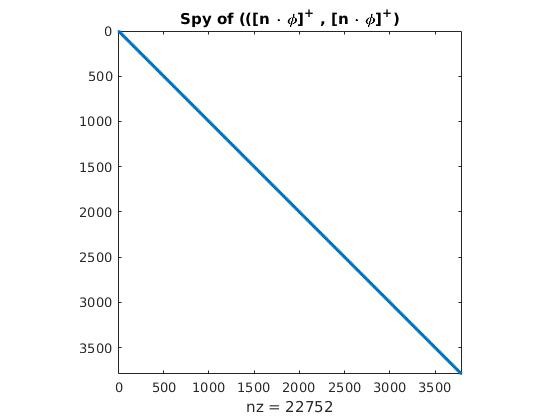
\includegraphics[width=\textwidth]{figure21.jpg}
    \label{fig:figure21}
	\caption{$((n \otimes \phi)^+,(n \otimes \phi)^+)_{\Gamma \cup \Gamma_D}$}      
  \end{minipage}\hfill
  \begin{minipage}[c]{0.5\textwidth}
    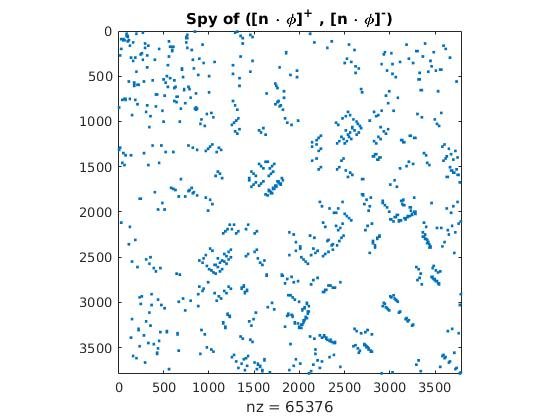
\includegraphics[width=\textwidth]{figure22.jpg}
    \label{fig:figure22}
	\caption{$((n \otimes \phi)^+,(n \otimes \phi)^-)_{\Gamma \cup \Gamma_D}$}      
  \end{minipage}\hfill
    \begin{minipage}[c]{0.5\textwidth}
    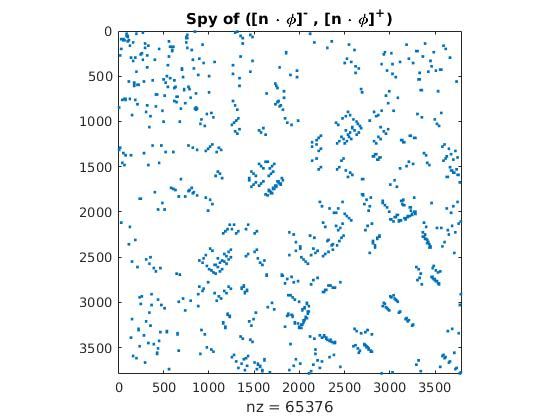
\includegraphics[width=\textwidth]{figure23.jpg}
    \label{fig:figure23}
	\caption{$((n \otimes \phi)^-,(n \otimes \phi)^+)_{\Gamma \cup \Gamma_D}$}      
  \end{minipage}\hfill
    \begin{minipage}[c]{0.5\textwidth}
    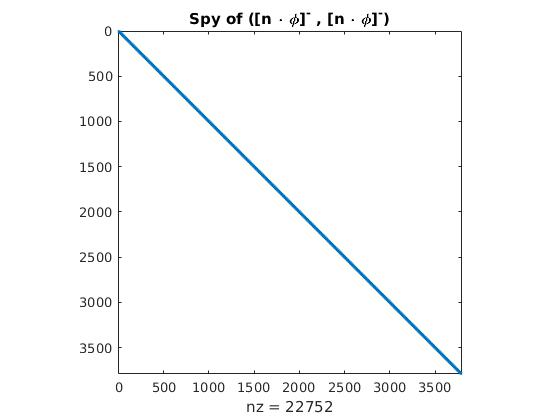
\includegraphics[width=\textwidth]{figure24.jpg}
    \label{fig:figure24}
	\caption{$((n \otimes \phi)^-,(n \otimes \phi)^-)_{\Gamma \cup \Gamma_D}$}      
  \end{minipage}\hfill
  \begin{subfigure}{\textwidth}	
\centering
  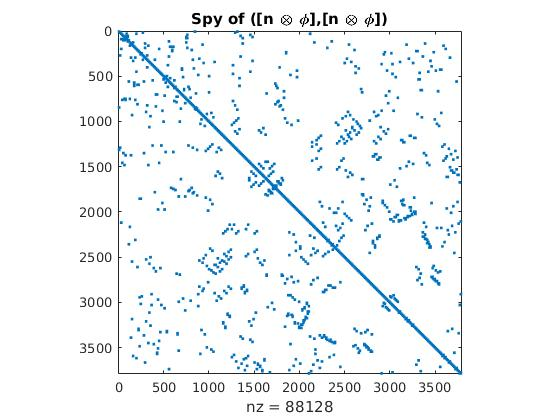
\includegraphics[width=\textwidth]{figure2.jpg}
  \caption{$([n \otimes \phi],[n \otimes \phi])_{\Gamma \cup \Gamma_D}$}
  \label{fig:figure2}
\end{subfigure}
\caption{Sparsity patterns of constituents of $([n \otimes \phi],[n \otimes \phi])_{\Gamma \cup \Gamma_D}$}
\caption{\label{figure_2_all}}
\end{figure}

\begin{figure}[H]
  \begin{minipage}[c]{0.5\textwidth}
    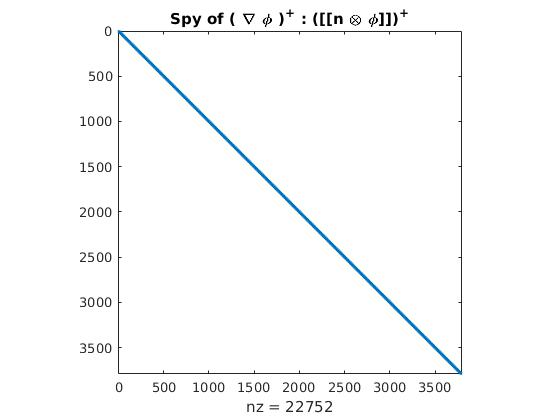
\includegraphics[width=\textwidth]{figure31.jpg}
\caption{$( \nabla \phi^+ ,(n \otimes \phi)^+)_{\Gamma \cup \Gamma_D}$}
  \label{fig:figure31}
  \end{minipage}\hfill
  \begin{minipage}[c]{0.5\textwidth}
    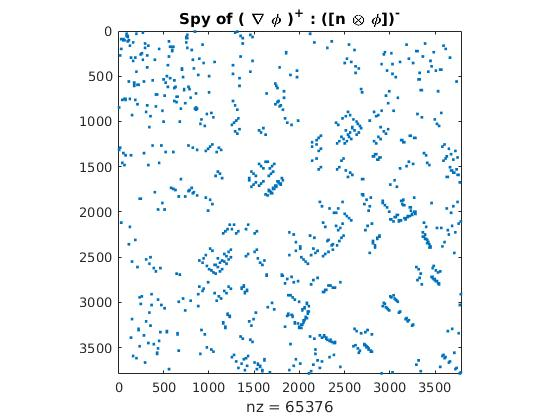
\includegraphics[width=\textwidth]{figure32.jpg}
  \caption{$( \nabla \phi^+ ,(n \otimes \phi)^-)_{\Gamma \cup \Gamma_D}$}
  \label{fig:figure32}
  \end{minipage}\hfill
    \begin{minipage}[c]{0.5\textwidth}
    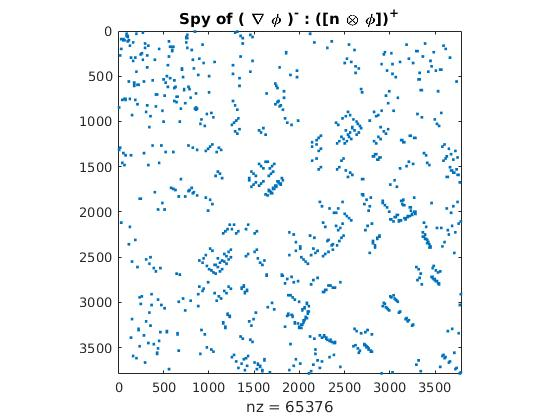
\includegraphics[width=\textwidth]{figure33.jpg}
  \caption{$( \nabla \phi^- ,(n \otimes \phi)^+)_{\Gamma \cup \Gamma_D}$}
  \label{fig:figure33}
  \end{minipage}\hfill
    \begin{minipage}[c]{0.5\textwidth}
    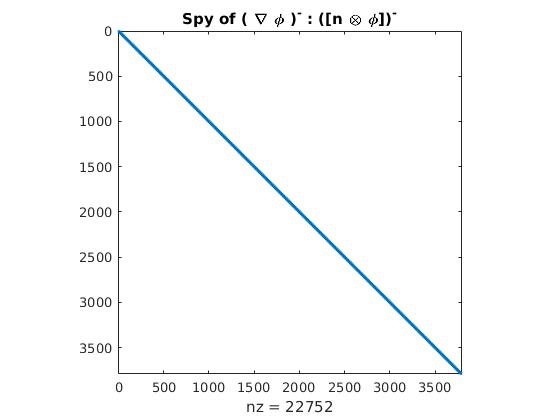
\includegraphics[width=\textwidth]{figure34.jpg}
  \caption{$( \nabla \phi^- ,(n \otimes \phi)^-)_{\Gamma \cup \Gamma_D}$}
  \label{fig:figure34}
  \end{minipage}\hfill
  \begin{subfigure}{\textwidth}	
\centering
  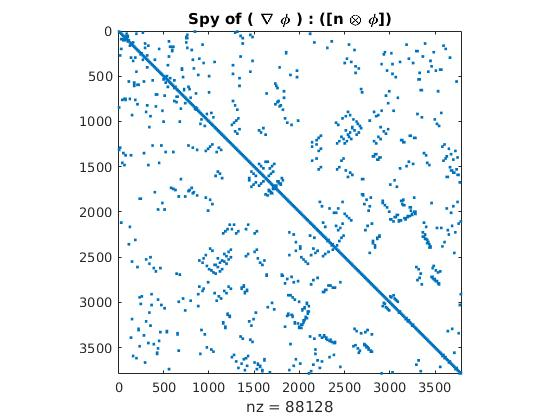
\includegraphics[width=\textwidth]{figure3.jpg}
  \caption{$(\lbrace \nabla \phi \rbrace,[n \otimes \phi])_{\Gamma \cup \Gamma_D}$}
  \label{fig:figure3}
\end{subfigure}
\caption{Sparsity patterns of constituents of $(\lbrace \nabla \phi  \rbrace,[n \otimes \phi])_{\Gamma \cup \Gamma_D}$}
\label{figure_3_all}
\end{figure}

\begin{figure}[H]
  \begin{minipage}[c]{0.5\textwidth}
    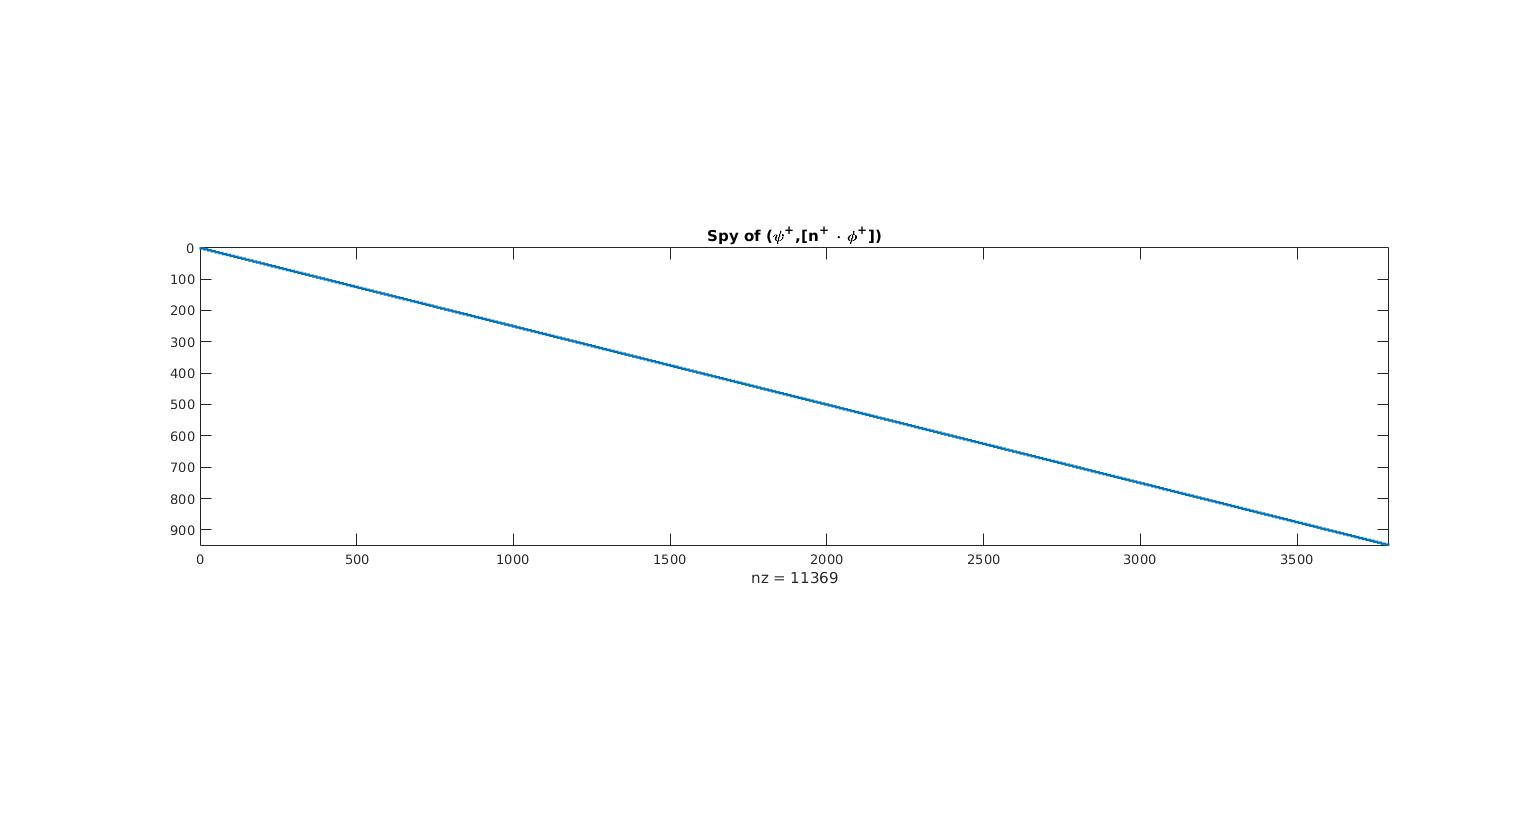
\includegraphics[width=\textwidth]{figure41.jpg}
  \caption{$( \psi^+ ,(n \cdot \phi)^+)_{\Gamma \cup \Gamma_D}$}
  \label{fig:figure41}
  \end{minipage}\hfill
  \begin{minipage}[c]{0.5\textwidth}
    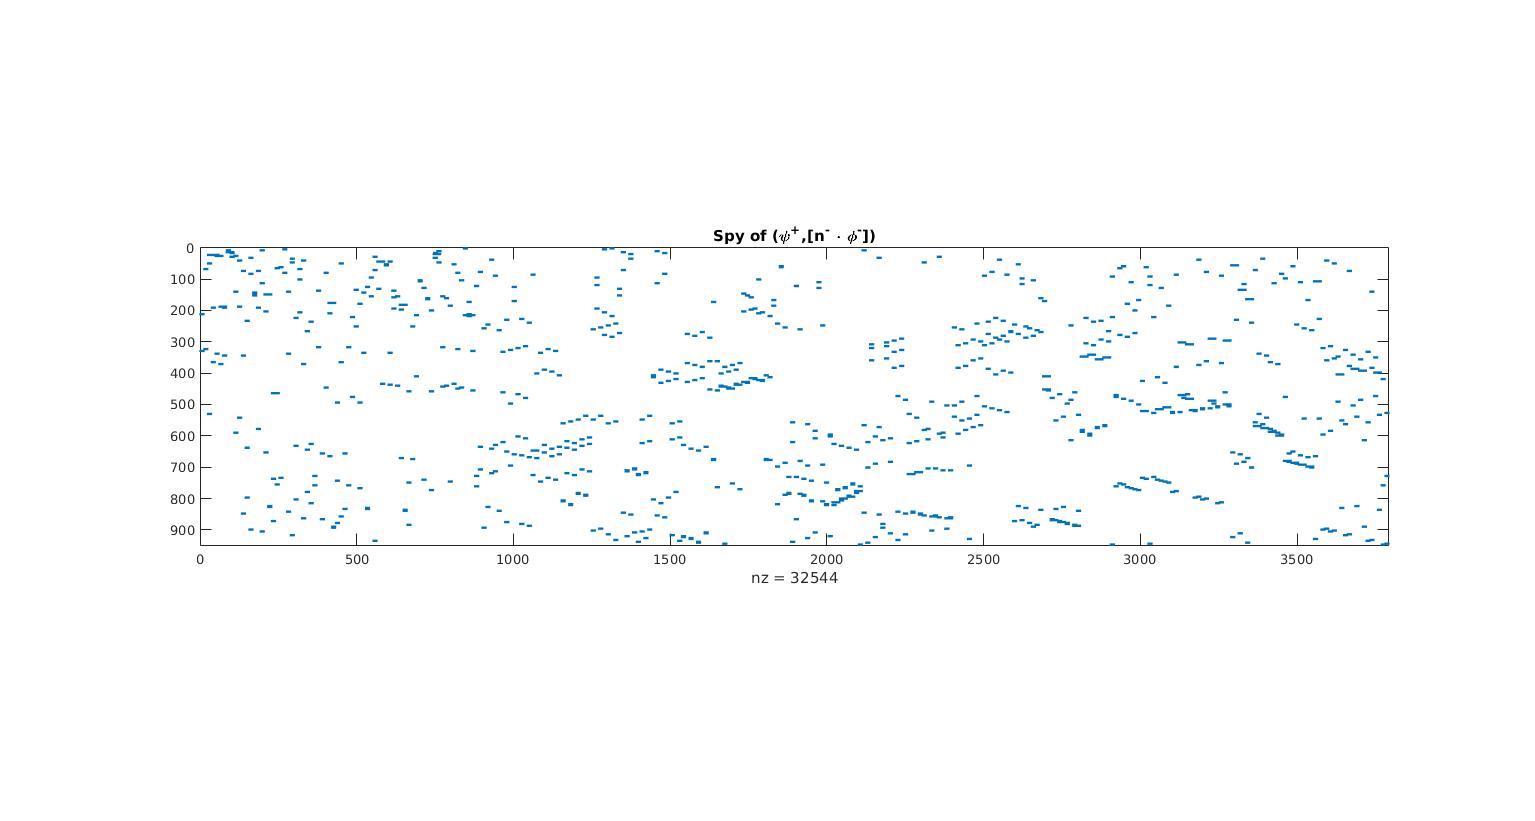
\includegraphics[width=\textwidth]{figure42.jpg}
  \caption{$( \psi^+ ,(n \cdot \phi)^-)_{\Gamma \cup \Gamma_D}$}
  \label{fig:figure42}
  \end{minipage}\hfill
    \begin{minipage}[c]{0.5\textwidth}
    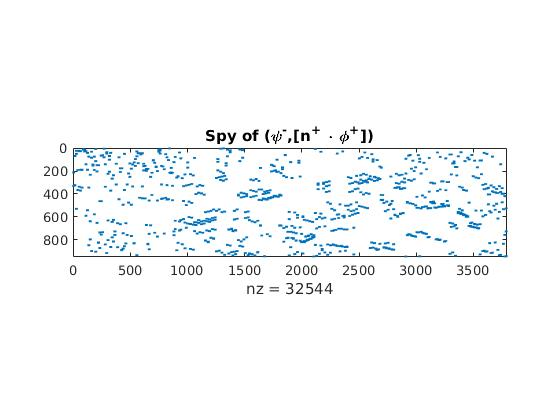
\includegraphics[width=\textwidth]{figure43.jpg}
  \caption{$( \psi^- ,(n \cdot \phi)^+)_{\Gamma \cup \Gamma_D}$}
  \label{fig:figure43}
  \end{minipage}\hfill
    \begin{minipage}[c]{0.5\textwidth}
    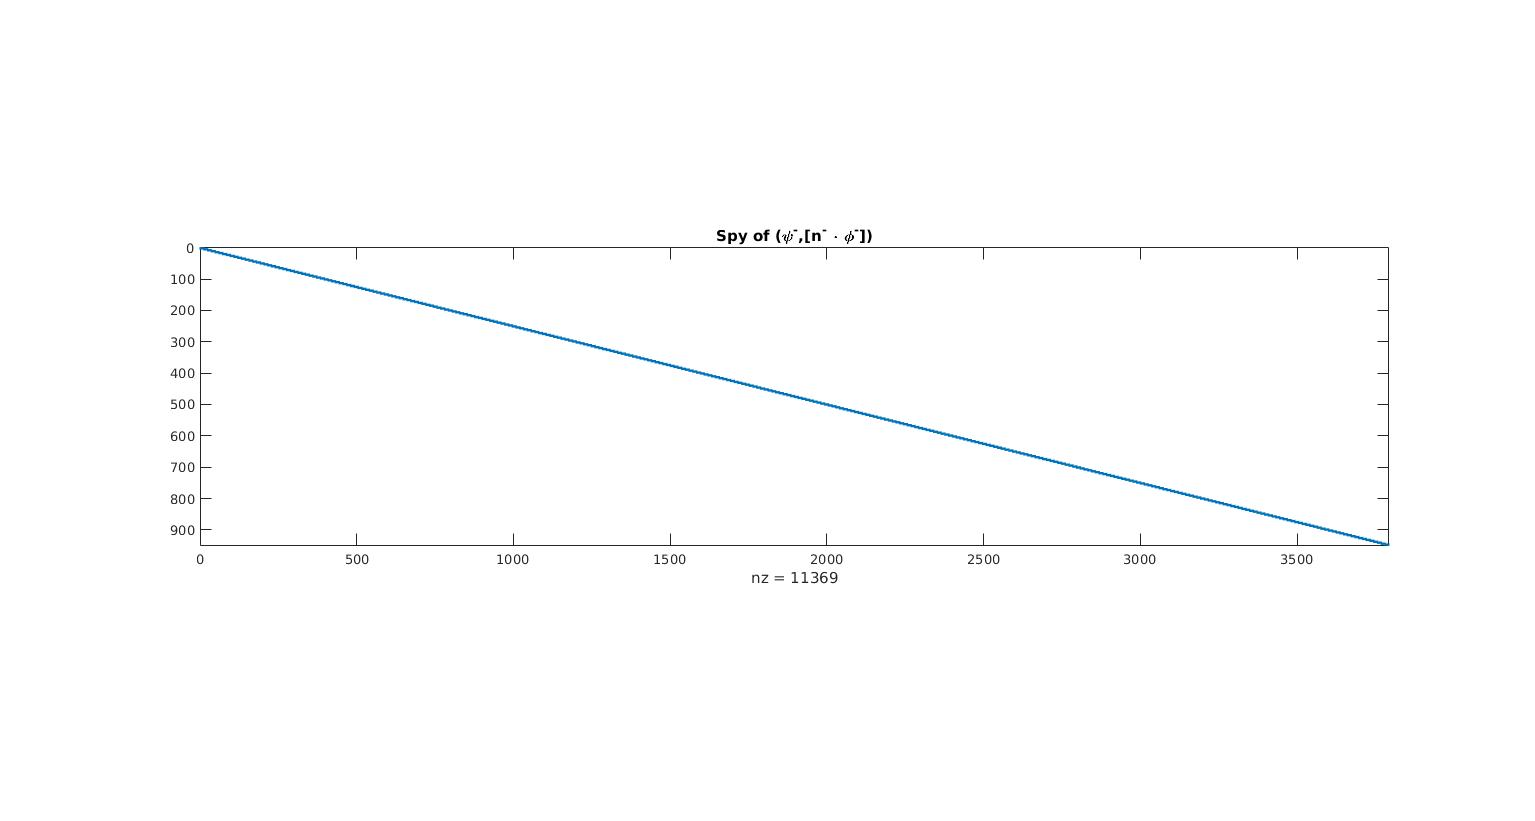
\includegraphics[width=\textwidth]{figure44.jpg}
  \caption{$( \psi^- ,(n \cdot \phi)^-)_{\Gamma \cup \Gamma_D}$}
  \label{fig:figure44}
  \end{minipage}\hfill
  \begin{subfigure}{\textwidth}	
\centering
  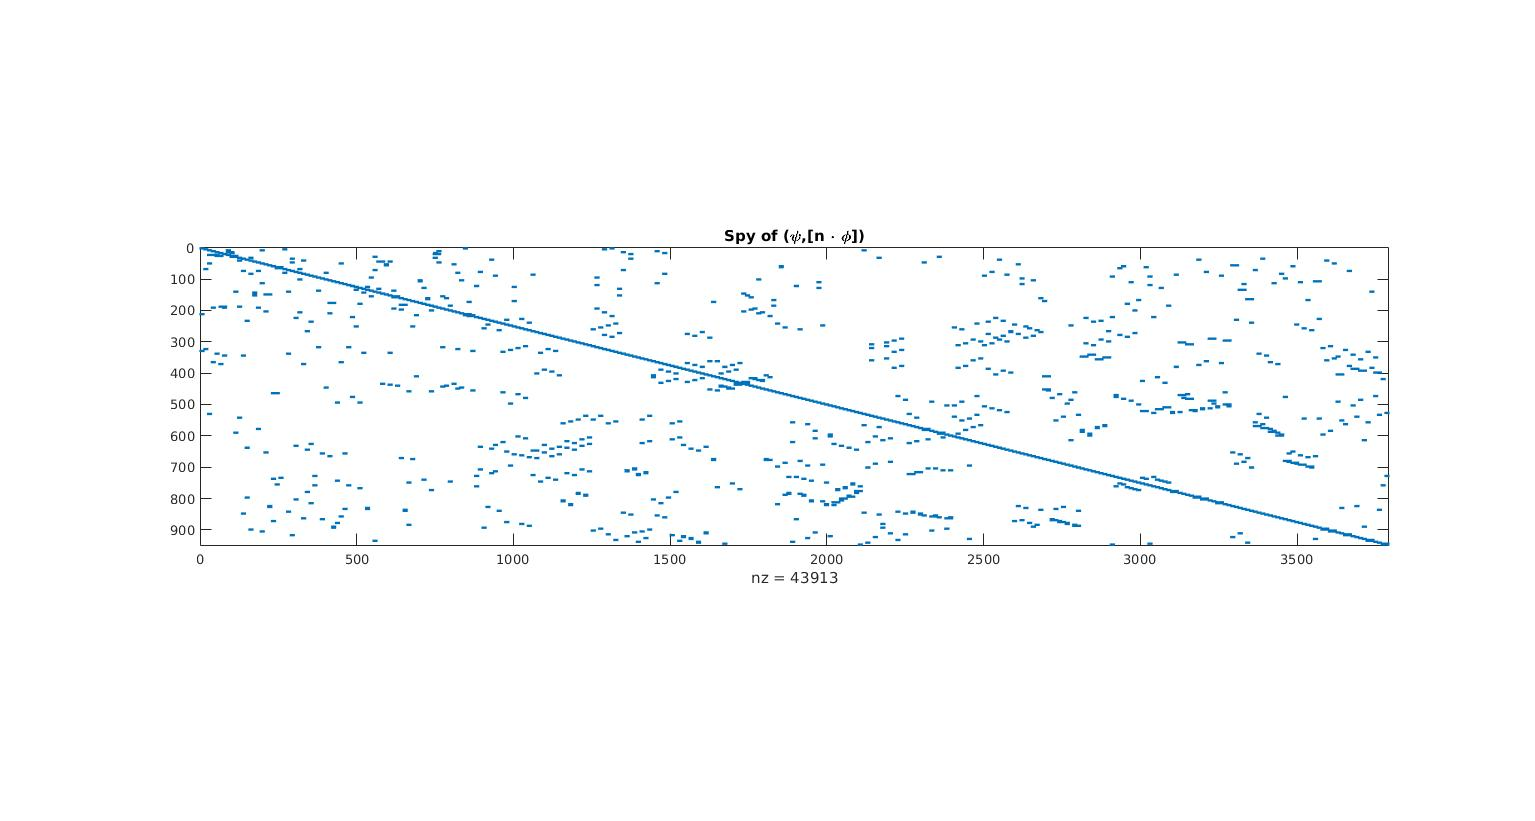
\includegraphics[width=\textwidth]{figure4.jpg}
  \caption{$(\lbrace \psi \rbrace ,[n \cdot \phi])_{\Gamma \cup \Gamma_D}$}
  \label{fig:figure4}
\end{subfigure}
\caption{Sparsity patterns of constituents of $(\lbrace \psi  \rbrace,[n \cdot \phi])_{\Gamma \cup \Gamma_D}$}
\label{figure_4_all}
\end{figure}

\begin{figure}[H]
\centering
  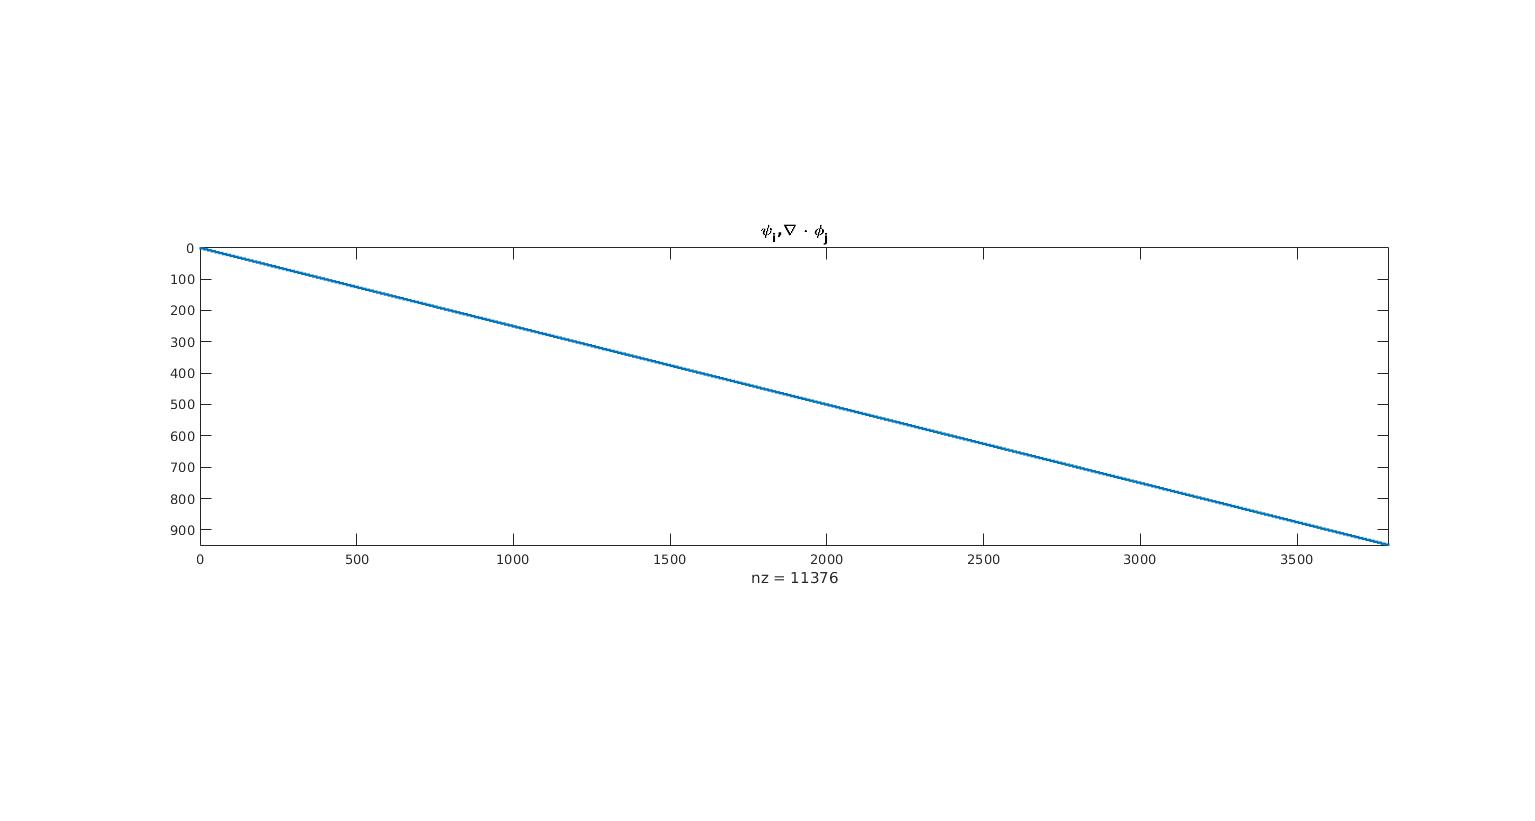
\includegraphics[width=\linewidth]{figure5.jpg}
  \caption{Sparsity pattern of $(\psi,\nabla \cdot \phi)$}
  \label{figure_5}
\end{figure}
\begin{figure}[H]
\centering
  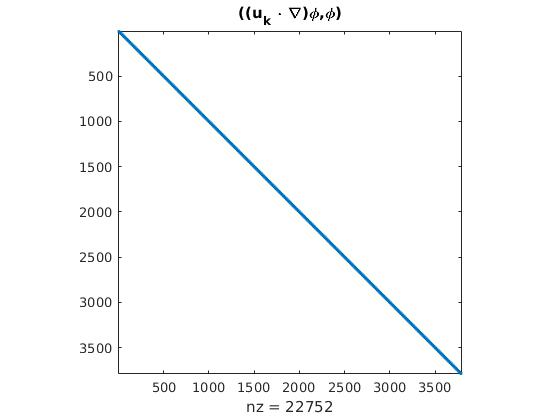
\includegraphics[width=\linewidth]{figure6.jpg}
  \caption{Sparsity pattern of $((u_k \cdot \nabla)\phi,\phi)$}
  \label{figure_6}
\end{figure}
\begin{figure}[H]
\centering
  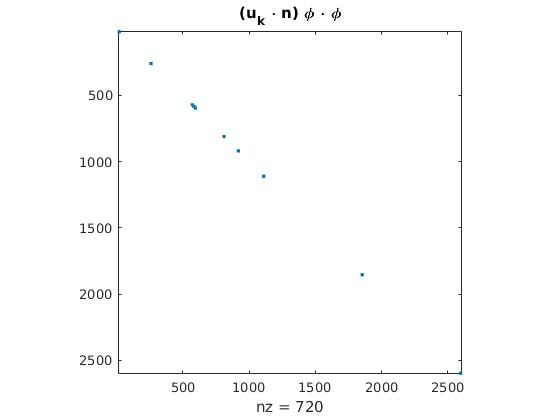
\includegraphics[width=\linewidth]{figure7.jpg}
  \caption{Sparsity pattern of $((u_k \cdot n)\phi,\phi)_{\Gamma_N}$}
  \label{figure_7}
\end{figure}
\begin{figure}[H]
\centering
  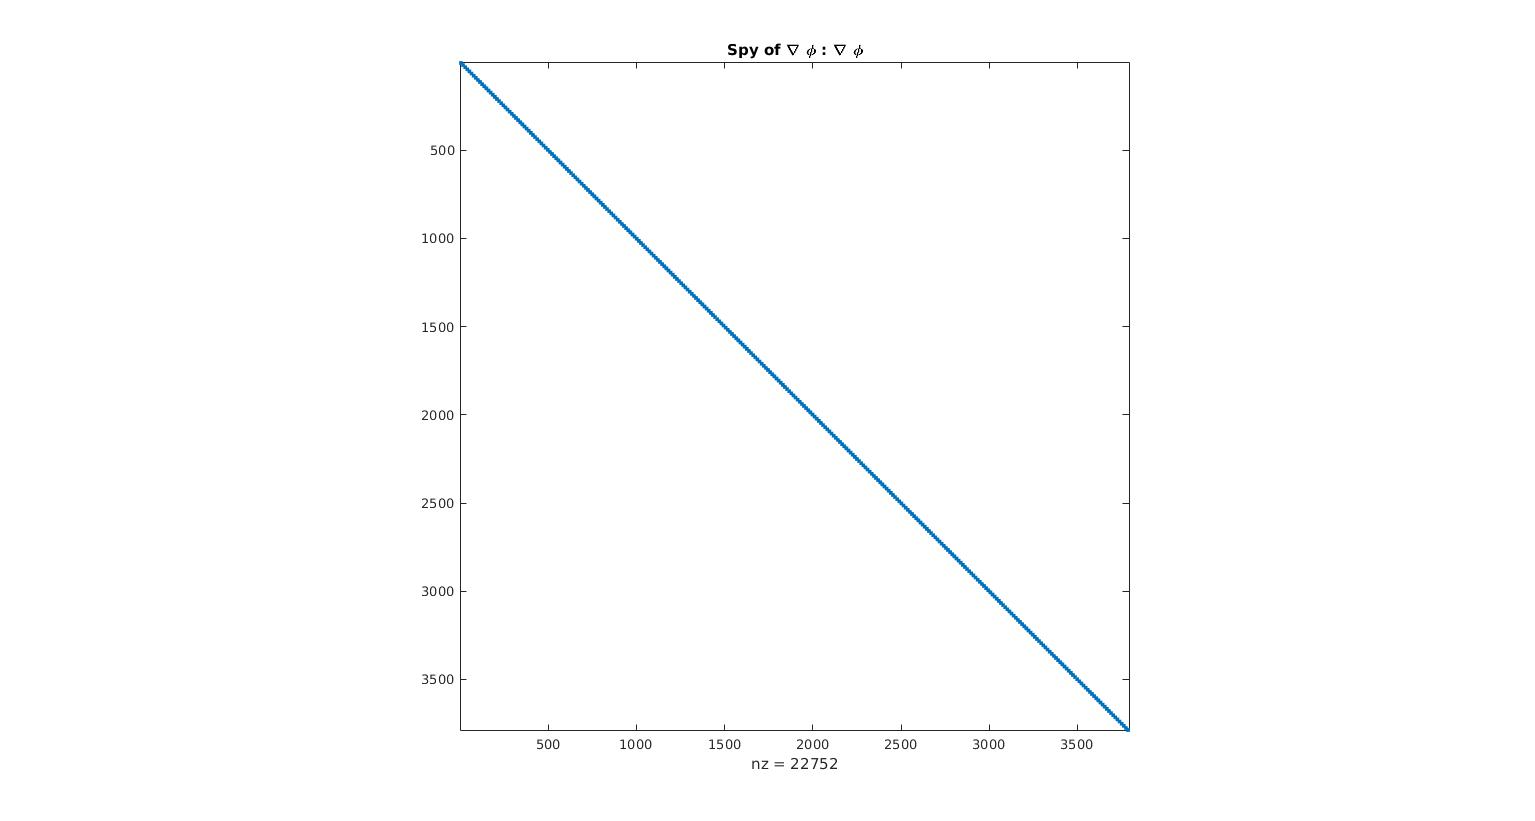
\includegraphics[width=\linewidth]{figure1.jpg}
  \caption{Sparsity pattern of $(\nabla \phi,\nabla \phi)$}
  \label{fig:sparsity_del_phi_del_phi}
\end{figure}
\begin{figure}[H]
\begin{subfigure}{\textwidth}
\centering
  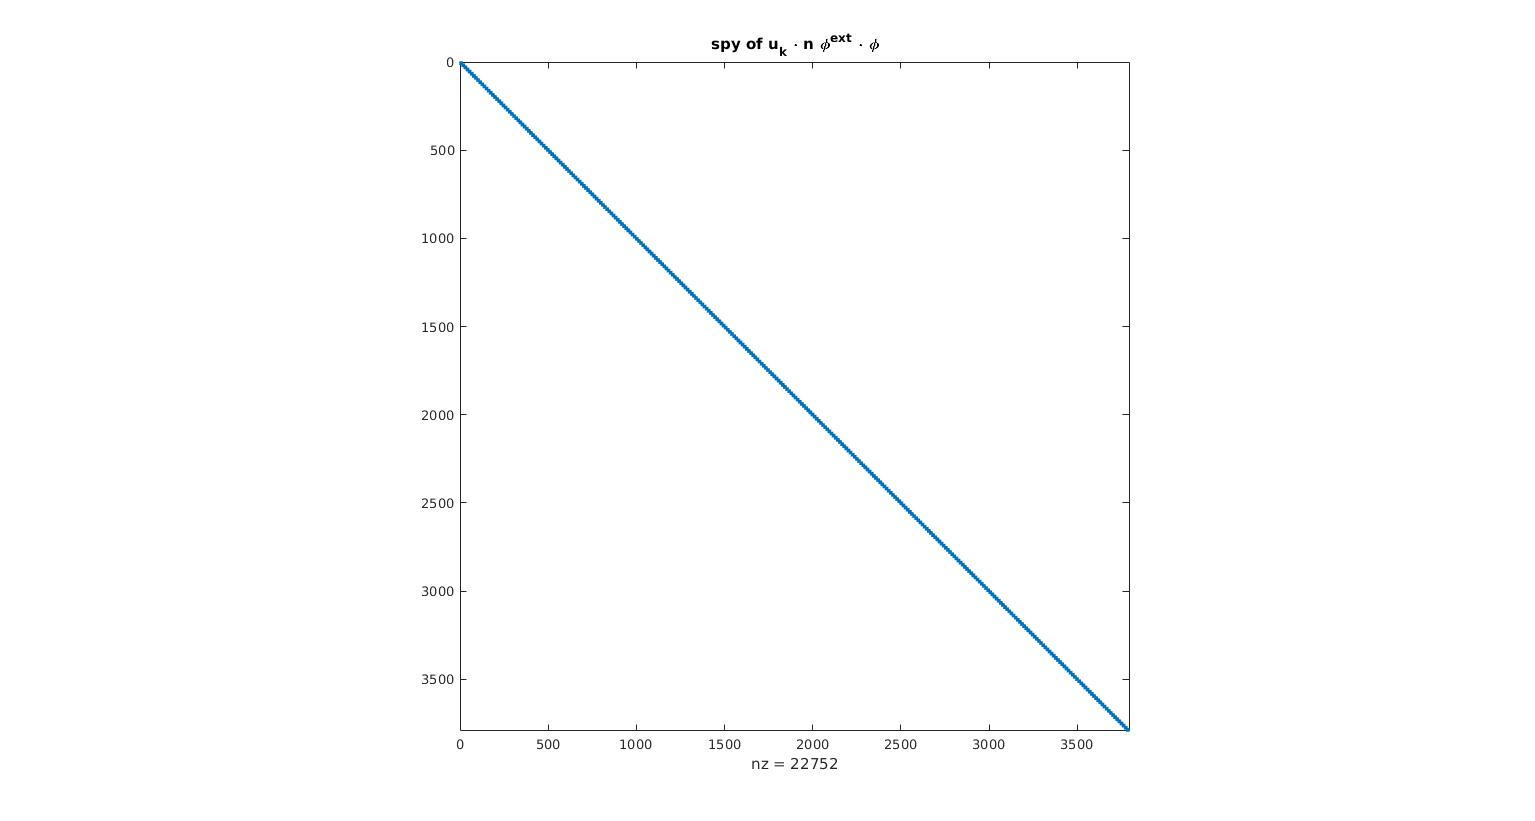
\includegraphics[width=\linewidth]{figure81.jpg}
  \caption{($((u_k \cdot n)\phi,\phi^{ext})_{\partial T \setminus \Gamma_N}$)}
  \label{figure_81}
\end{subfigure}
\begin{subfigure}{\textwidth}	
\centering
  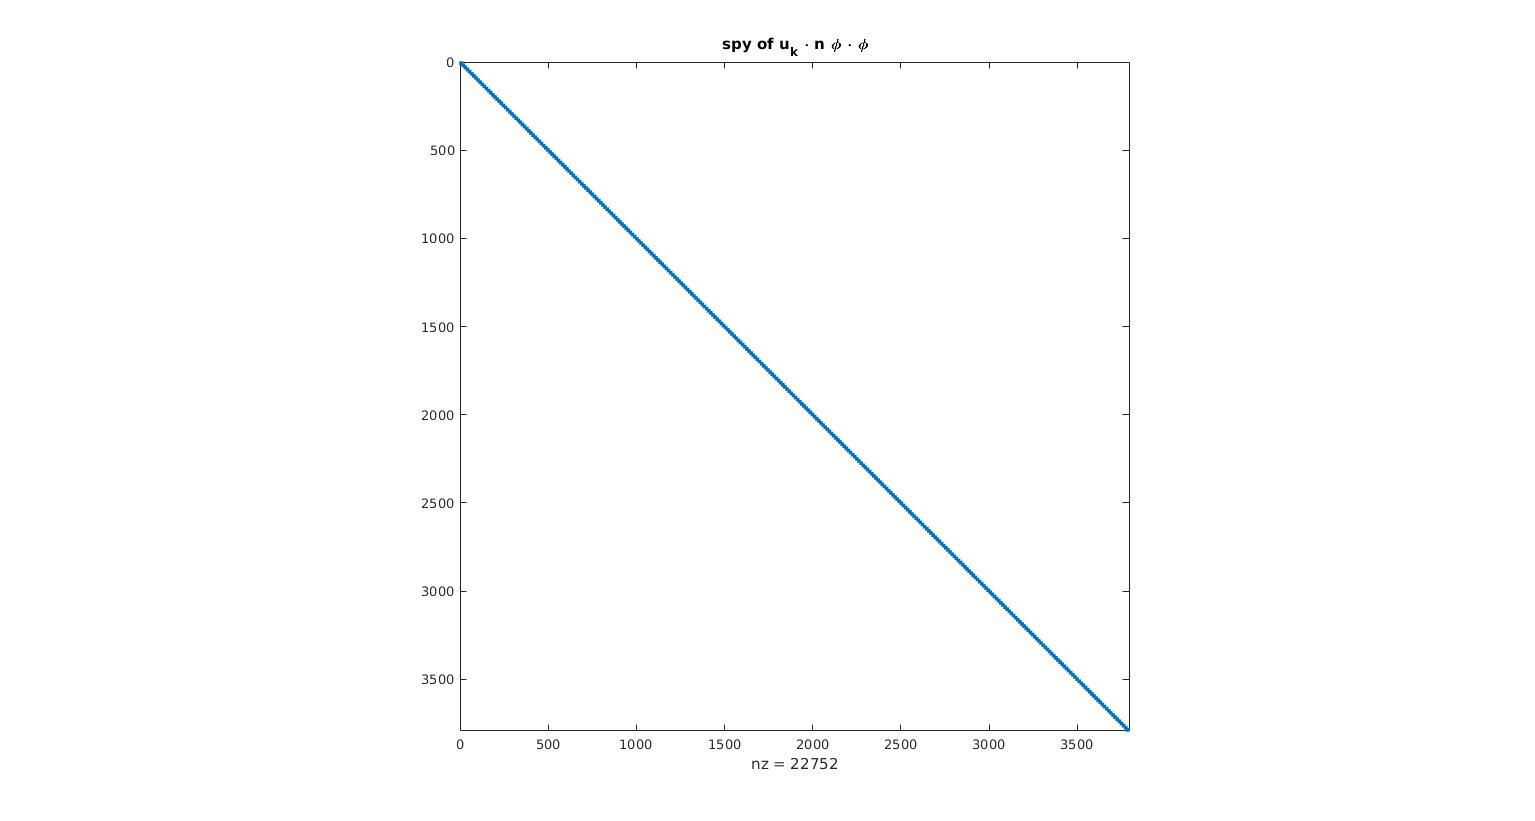
\includegraphics[width=\linewidth]{figure82.jpg}
  \caption{($((u_k \cdot n)\phi,\phi)_{\partial T \setminus \Gamma_N}$)}
  \label{figure_82}
\end{subfigure}
\begin{subfigure}{\textwidth}	
\centering
  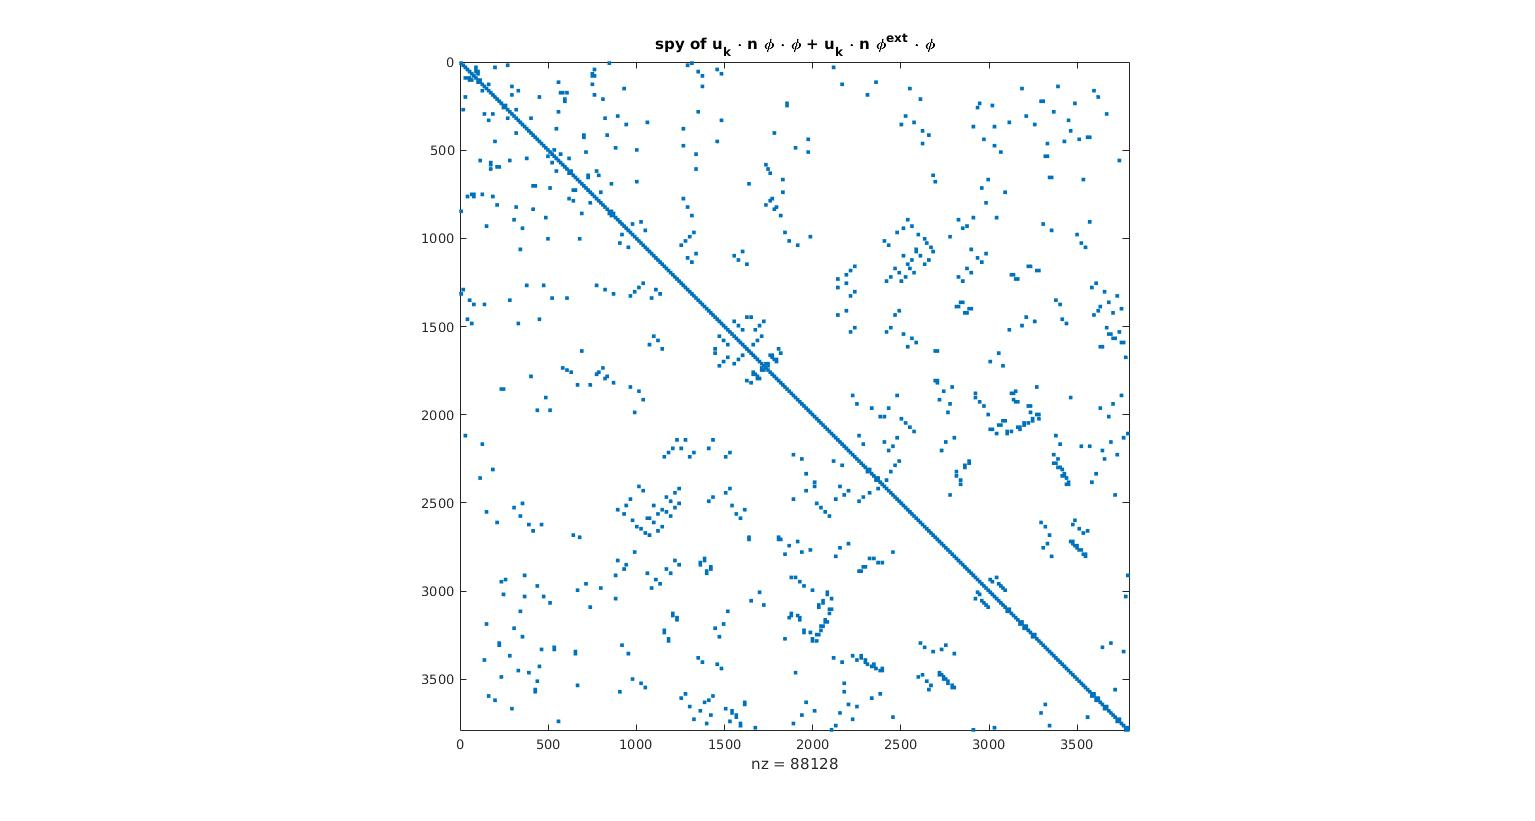
\includegraphics[width=\linewidth]{figure8.jpg}
  \caption{$((u_k \cdot n)\phi,\phi^{ext})_{\partial T \setminus \Gamma_N} + ((u_k \cdot n)\phi,\phi)_{\partial T \setminus \Gamma_N}$}
  \label{figure_8}
\end{subfigure}
\caption{Sparsity patterns of constituents of $((u_k \cdot n)\phi,\phi^{ext})_{\partial T \setminus \Gamma_N} + ((u_k \cdot n)\phi,\phi)_{\partial T \setminus \Gamma_N}$}
\label{figure_8_all}
\end{figure}

\begin{figure}[H]
\begin{subfigure}{\textwidth}
\centering
  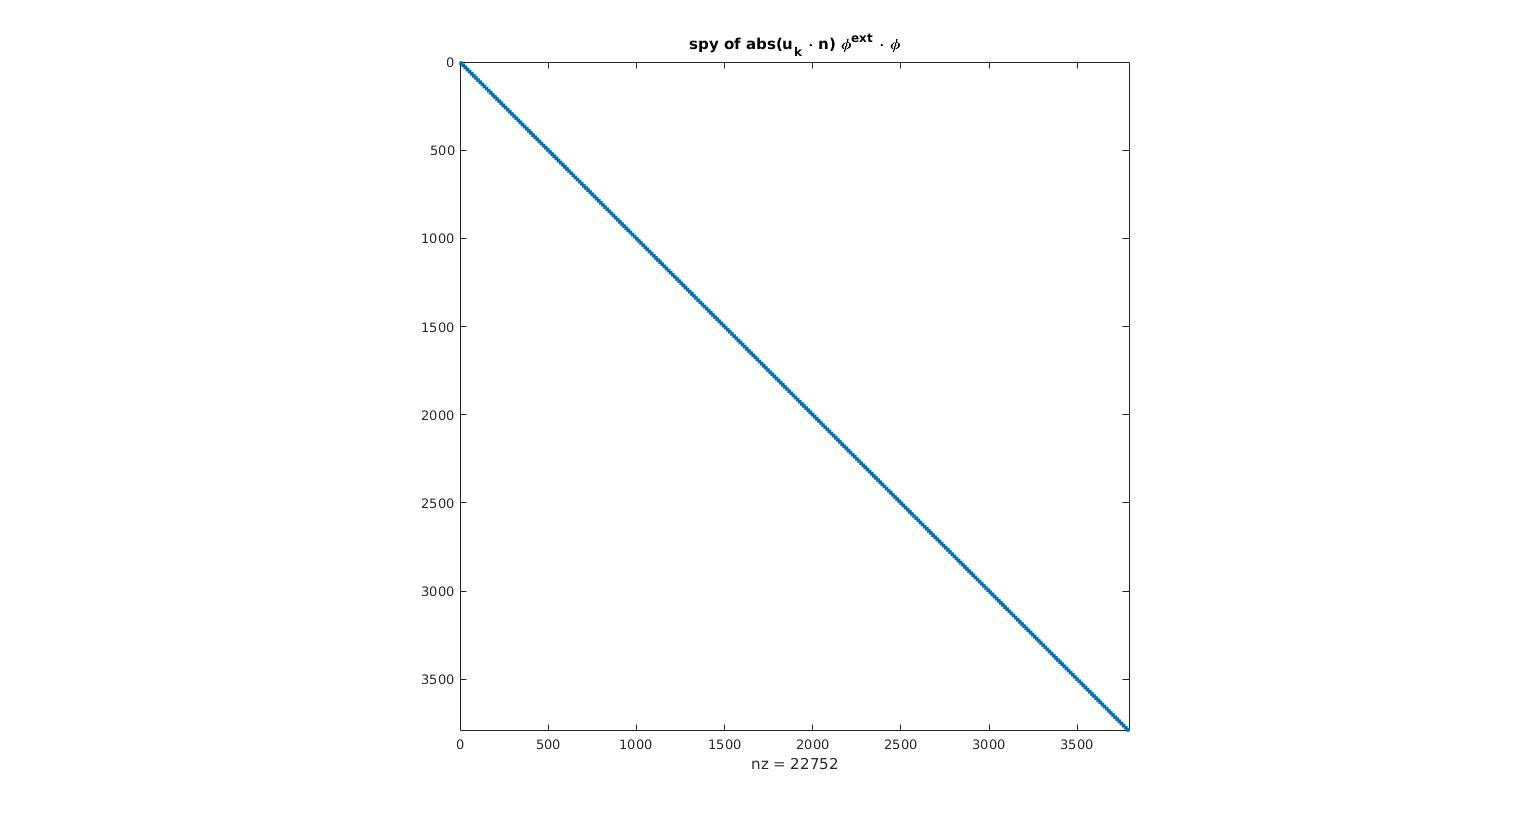
\includegraphics[width=\linewidth]{figure91.jpg}
  \caption{($(abs(u_k \cdot n)\phi,\phi^{ext})_{\partial T \setminus \Gamma_N}$)}
  \label{figure_91}
\end{subfigure}
\begin{subfigure}{\textwidth}	
\centering
  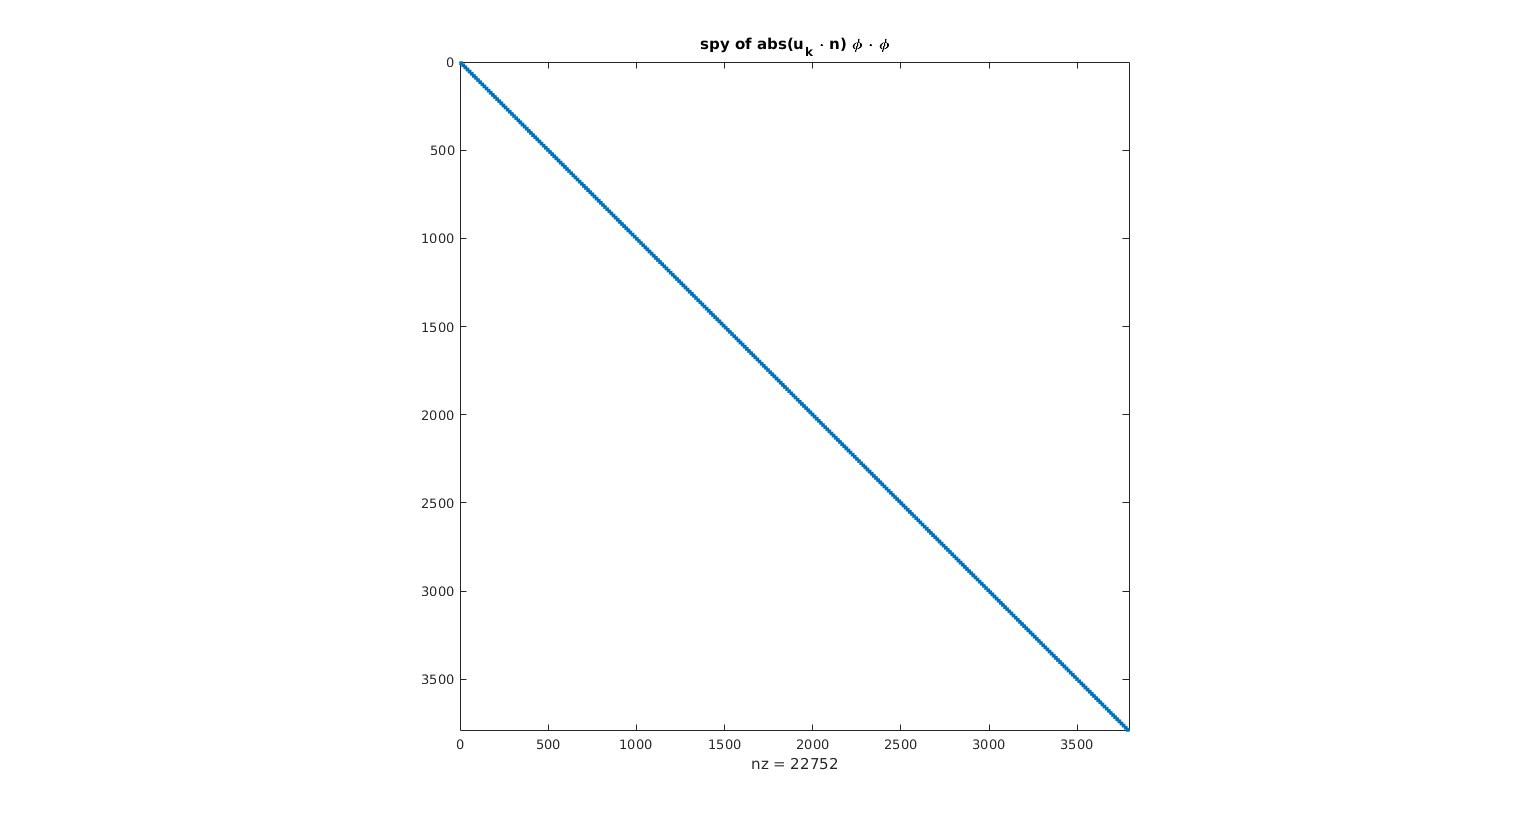
\includegraphics[width=\linewidth]{figure92.jpg}
  \caption{($(abs(u_k \cdot n)\phi,\phi)_{\partial T \setminus \Gamma_N}$)}
  \label{figure_92}
\end{subfigure}
\begin{subfigure}{\textwidth}	
\centering
  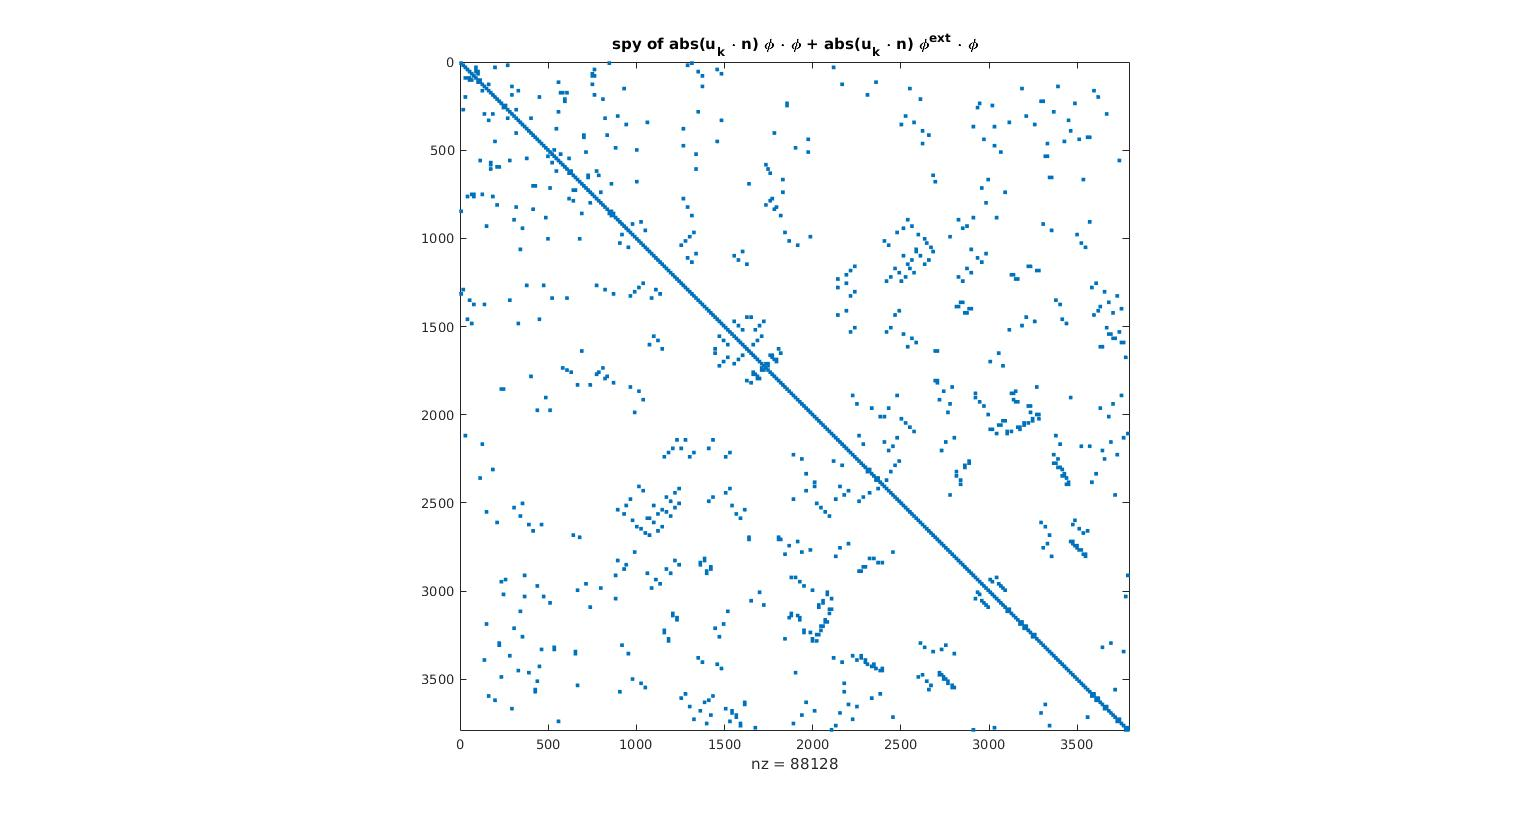
\includegraphics[width=\linewidth]{figure9.jpg}
  \caption{$(abs(u_k \cdot n)\phi,\phi^{ext})_{\partial T \setminus \Gamma_N} + (abs(u_k \cdot n)\phi,\phi)_{\partial T \setminus \Gamma_N}$}
  \label{figure_9}
\end{subfigure}
\caption{Sparsity patterns of constituents of $(abs(u_k \cdot n)\phi,\phi^{ext})_{\partial T \setminus \Gamma_N} + (abs(u_k \cdot n)\phi,\phi)_{\partial T \setminus \Gamma_N}$}
\label{figure_9_all}
\end{figure}

\chapter{Numerical experiments}

This chapter discusses results obtained by performing the numerical experiments on the discontinuous Galerkin formulation of the Stokes equation and the Navier Stokes equation.

\section{Error definitions}

The error is the difference, measured in a suitable norm, between the true solution and an approximated or computed solution. It is also a measure of how closely the implemented scheme simulates the physical nature of the problem. A correct numerical scheme should converge to the actual solution when the number of degrees of freedom are increased. The degrees of freedom can be increased either by discretizing the domain further ($h-$convergence) or by increasing the degree of the basis functions ($p-$convergence). If $P_h$ is the computed solution and $P$ is the true solution, the error in the $W$-norm is defined as,

\begin{equation} \label{error_definition}
P_{error,W} = ||P - P_h||_{W} \quad \mathrm{.}
\end{equation}

In the present analysis, we measure the error in the $L^2$ norm and the $H_0$ semi norm and present results of an $h-$convergence test.

The $L^2$ norm of the error is measured as,\begin{equation}
P_{error,L^2} = \int_{\Omega} |P - P_h|^2 \quad \mathrm{.}
\end{equation}

The $H_0$ semi norm of the error is defined as,\begin{equation}
P_{error,H_0} = \sum_{k=1}^{nel} \int_{\tau_k} |\nabla P - \nabla P_h|^2 \quad \mathrm{.}
\end{equation}

We use the notations from the Section \ref{n_s_ch3} and the Section \ref{Stokes_flow_ch3}.

\section{Stokes flow}\label{Stokes-ch5}

\subsection{Properties of the stiffness matrix}

We recall now some conclusions from the Section \ref{property_stif_mat_stokes} and the Section \ref{property_stif_mat_navier}. The present code provides a routine \verb|stiffness_matrix_test| which, \\

1. checks whether the coefficient matrix $K$ is symmetric and the number of non positive eigenvalues. The number of non positive eigenvalues should be same as the number of pressure degrees of freedom. It also provides eigenvalues and eigenvectors as output,\\

2. calculates the condition number of the coefficient matrix $K$, \\

3. determines the rank of coefficient matrix $K$.\\

\verb|stiffness_matrix_test| can also be used for the matrix $A$ by giving the matrix $A$ as input. In this case the matrix should be symmetric and all eigenvalues should be positive.\\

We consider Stiffness matrix $K$ symmetric, if $||K-K^T||_2 \leq tol$, where $tol$ is some specified tolerance. Due to round off error, $tol > 0$.   

\subsection{Analytical example}

The domain considered for this example is the unit square [0,1] $\times$ [0,1] in the $x-y$ plane. 
The boundary ${x=0}$ is dirichlet boundary with inflow velocity at point $(0,y)$ as $u = (y(1-y), 0)$. The boundaries ${y = 0}$ and ${y = 1}$ are Dirichlet boundaries with no slip or zero velocity condition. The boundary ${x = 1}$ is a Neumann boundary with zero Neumann value i.e. $t = (0, 0)$. The source term is $f = (2 \nu - 1, 0)$. The analytical solution for pressure and velocity reads as,

\begin{center}

\begin{equation}
p = (1 - x)
\end{equation}

\begin{equation} 
 u = (y(1-y), 0) \quad \textrm{.}
\end{equation}

\end{center}

The results of an $h-$convergence test in the $L^2$ norm with velocity polynomial degree $D=2$ and pressure polynomial degree $D-1 = 2$ is presented in Figures \ref{fig:vel_stoke_conv}, \ref{fig:vel_stoke_conv_log}, \ref{fig:pre_stoke_conv} and \ref{fig:pre_stoke_conv_log} and in the $H_0$ semi norm is presented in Figures \ref{fig:vel_stoke_conv_h0}, \ref{fig:vel_stoke_conv_log_h0}, \ref{fig:pre_stoke_conv_h0} and \ref{fig:pre_stoke_conv_log_h0}. We see almost linear converegnce. \\

We also present results of $p-$convergence test in $L^2$ norm and $H_0$ semi norm for velocity and in $L^2$ norm for pressure (Figures \ref{p_convergence_velocity_l2}, \ref{p_convergence_velocity_h0}, \ref{p_convergence_pressure_l2}). As can be seen the higher polynomial degree does not necessarily mean more accurate solution. However, the convergence rate increases with polynomial degree and beyond certain step size, the higher polynomial provides more accurate solution.

\begin{figure}
\begin{subfigure}{\textwidth}
\centering
  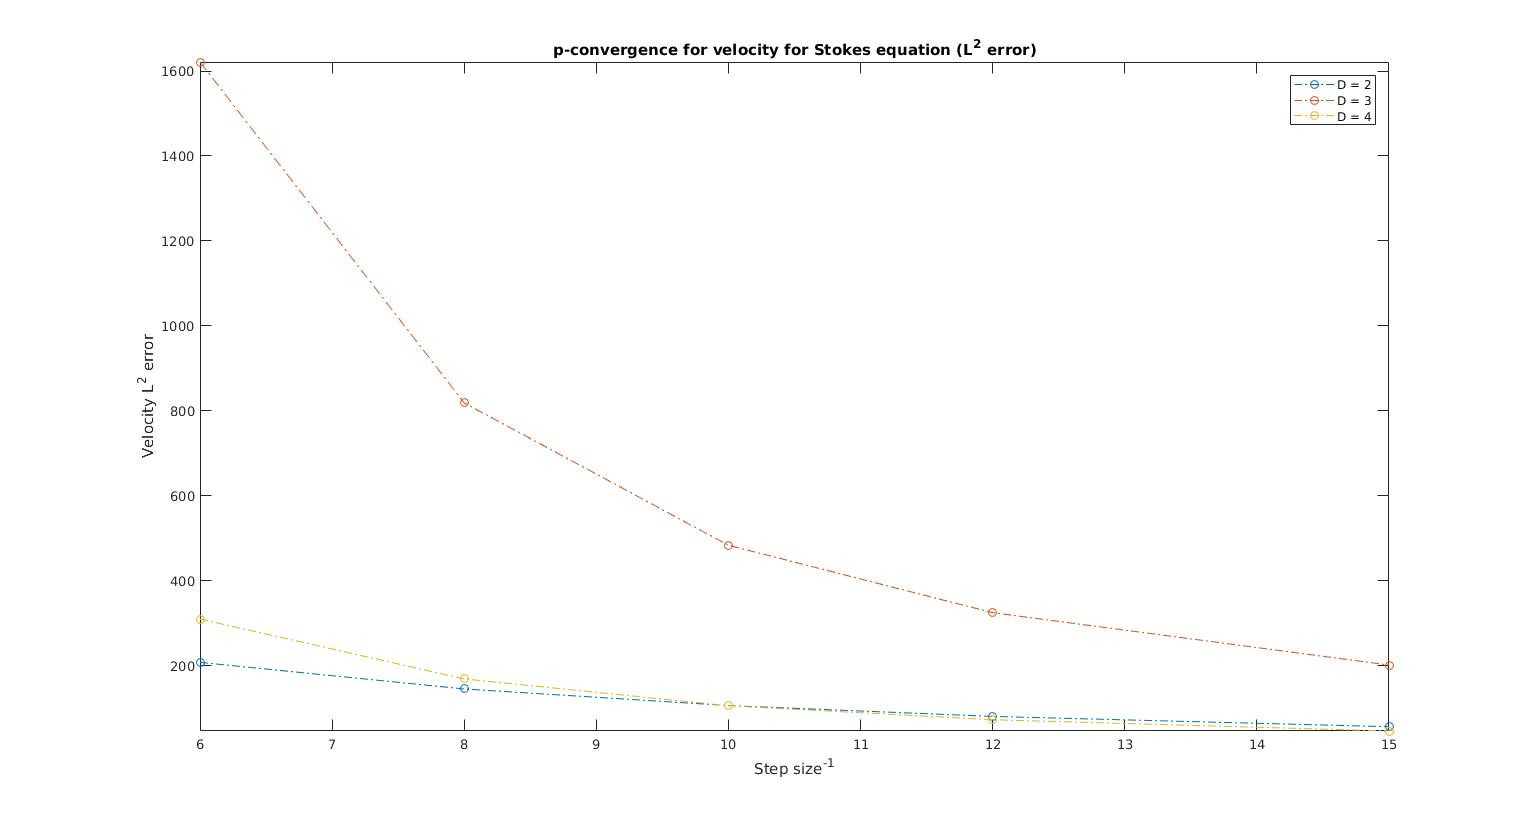
\includegraphics[width=\linewidth]{p_conv_velocity_l2_stokes.jpg}
  \caption{($p-$convergence for velocity in $L^2$ norm for Stokes flow)}
  \label{p_convergence_velocity_l2}
\end{subfigure}
\begin{subfigure}{\textwidth}
\centering
  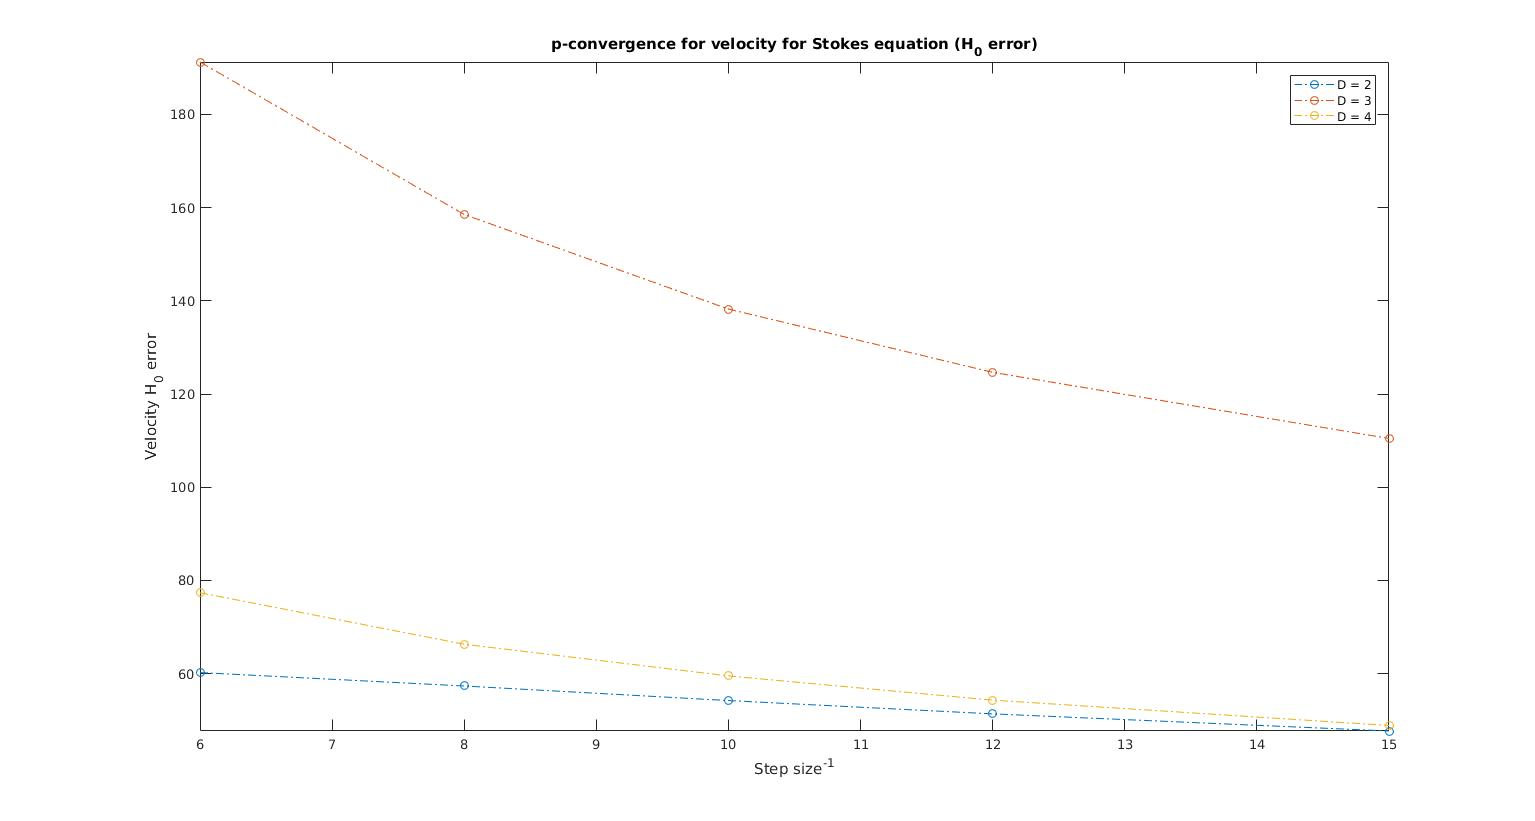
\includegraphics[width=\linewidth]{p_conv_velocity_h0_stokes.jpg}
  \caption{($p-$convergence for velocity in $H_0$ semi norm for Stokes flow)}
  \label{p_convergence_velocity_h0}
\end{subfigure}
\begin{subfigure}{\textwidth}
\centering
  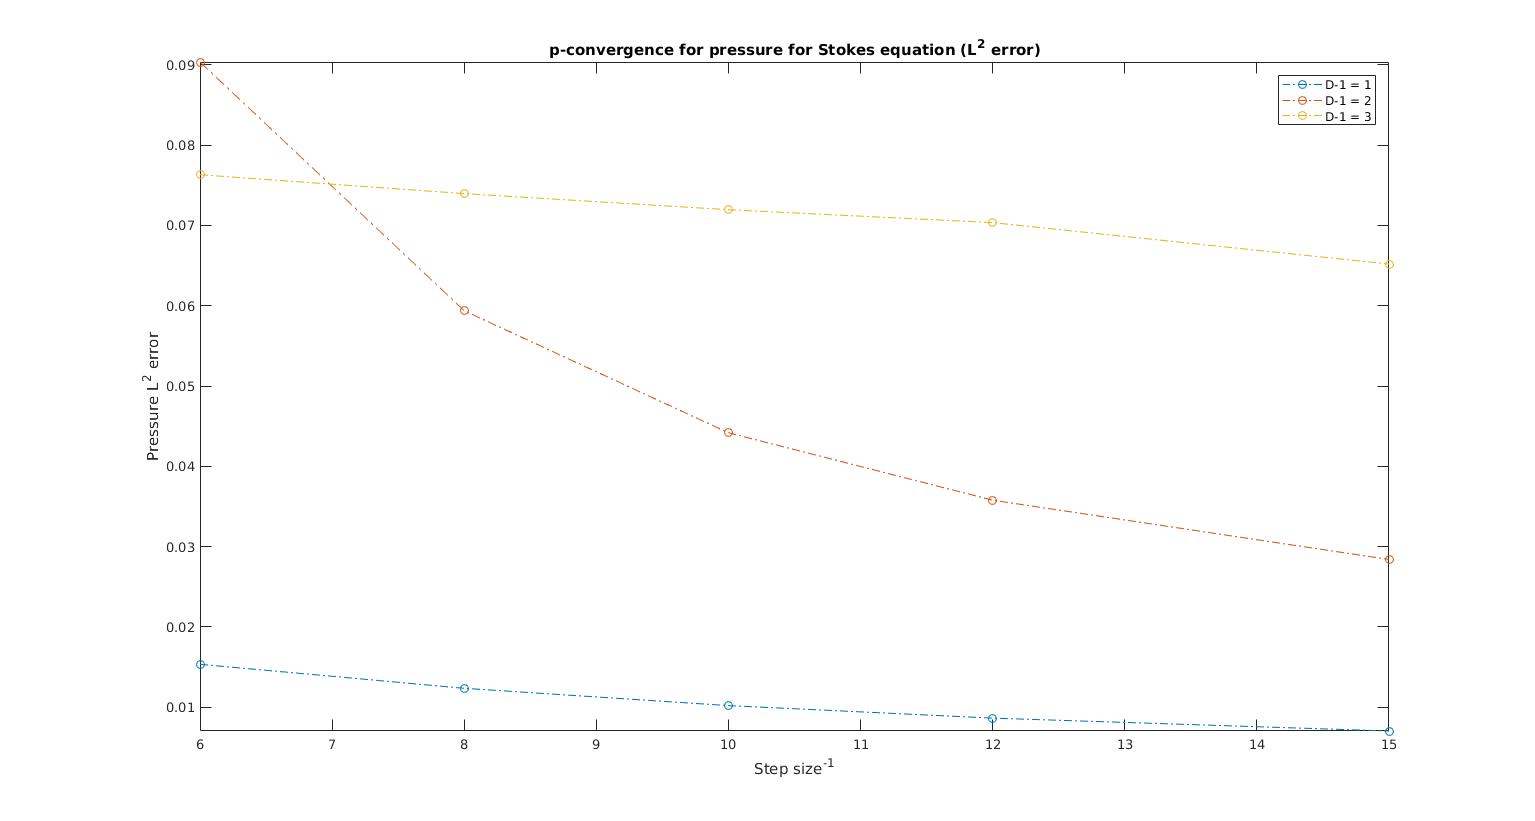
\includegraphics[width=\linewidth]{p_conv_pressure_l2_stokes.jpg}
  \caption{($p-$convergence for pressure in $L^2$ norm for Stokes flow)}
  \label{p_convergence_pressure_l2}
\end{subfigure}
\caption{$p-$convergence for Stokes flow}
\label{p_conv_stokes_flow}
\end{figure}


We now present additional examples and check whether the implementation of the Stokes flow is capable of reproducing the physics of the problem.

\subsection{Lid-driven cavity problem} \label{lid_driven_cavity_stokes}

We next present a benchmark $CFD$ problem, the Lid-driven cavity flow \cite{Montlaur2}. We solve the Stokes flow on the unit square [0,1] $\times$ [0,1] in the $x-y$ plane. On boundaries ${x = 0}, {x = 1}$ and ${y = 0}$, we impose no slip or zero velocity Dirichlet condition. On ${y = 1}$, we impose Dirichlet condition with Dirichlet velocity,
\begin{equation}
u = (10x,0)^T \quad \textrm{for} \quad 0 \leq x \leq 0.1
\end{equation}
\begin{equation}
u = (1,0)^T \quad \textrm{for} \quad 0.1 \leq x \leq 0.9
\end{equation}
\begin{equation}
u = (10 - 10x,0)^T \quad \textrm{for} \quad 0.9 \leq x \leq 1 \quad \textrm{.}
\end{equation}

The results are shown in Figures \ref{stoke_bicgstab_lid}, \ref{stoke_minres_lid} and \ref{stoke_schur_lid}. The results are found to be in agreement with literature i.e. boundary layer formation at the no slip boundaries and shape of streamline. 

\subsection{Flow over cylinder} \label{flow_over_cylinder_stokes}

The domain considered for this example is the unit square [0,1] $\times$ [0,1] with a cut out cylinder of diameter 0.2 centered at $(0.5,0.5)$ i.e. the center of cylinder coincides with the center of the square in the $x-y$ plane. The boundary ${x=0}$ is Dirichlet boundary with inflow velocity at point $(0,y)$ as $u = (y(1-y), 0)$. The boundaries ${y = 0}$ and ${y = 1}$ are Dirichlet boundaries with no slip or zero velocity condition. The boundary ${x = 1}$ is a Neumann boundary with zero Neumann value i.e. $t = (0, 0)$. The source term is $f = (0, 0)$. Figures \ref{flow_over_cylinder_bicgstab}, \ref{flow_over_cylinder_minres} and \ref{flow_over_cylinder_schur} give physically relevant result for example, low pressure zone after cylinder, high pressure zone before cylinder and wake zone after cylinder for velocity.

\begin{figure}
\begin{subfigure}{\textwidth}	
  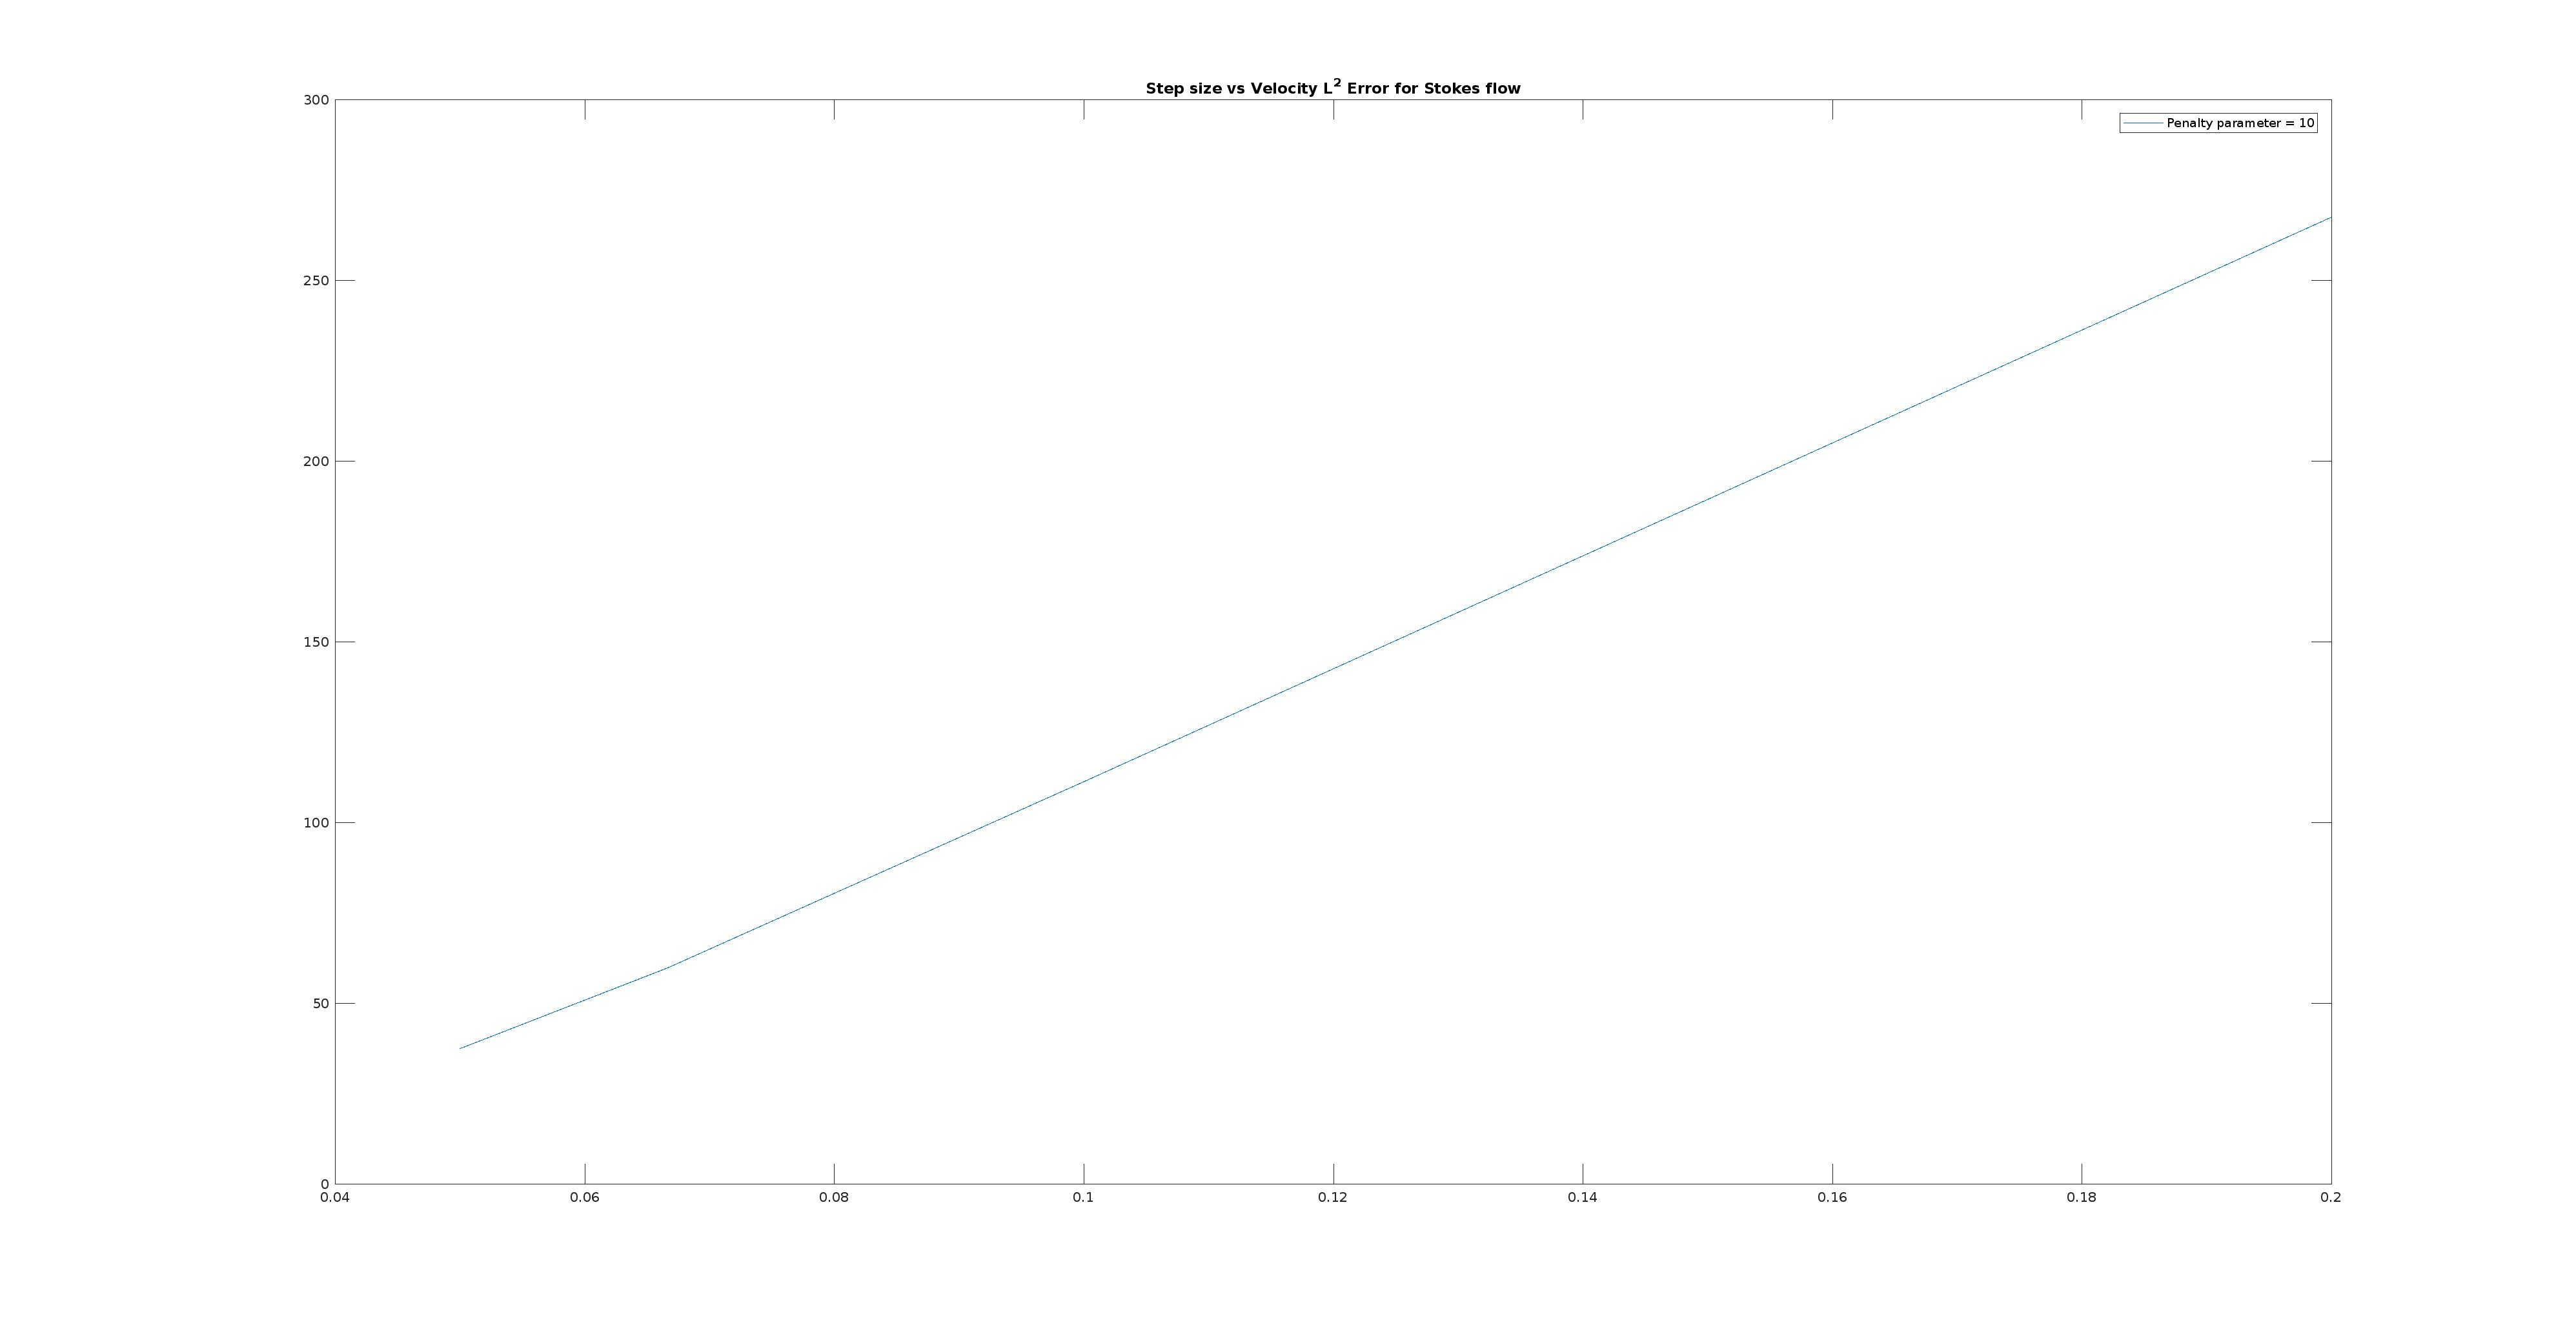
\includegraphics[width=\linewidth]{l2_velocity_stokes.jpg}
  \caption{$h-$ convergence test for velocity $L^2$ error}
  \label{fig:vel_stoke_conv}
\end{subfigure}
\begin{subfigure}{\textwidth}	
  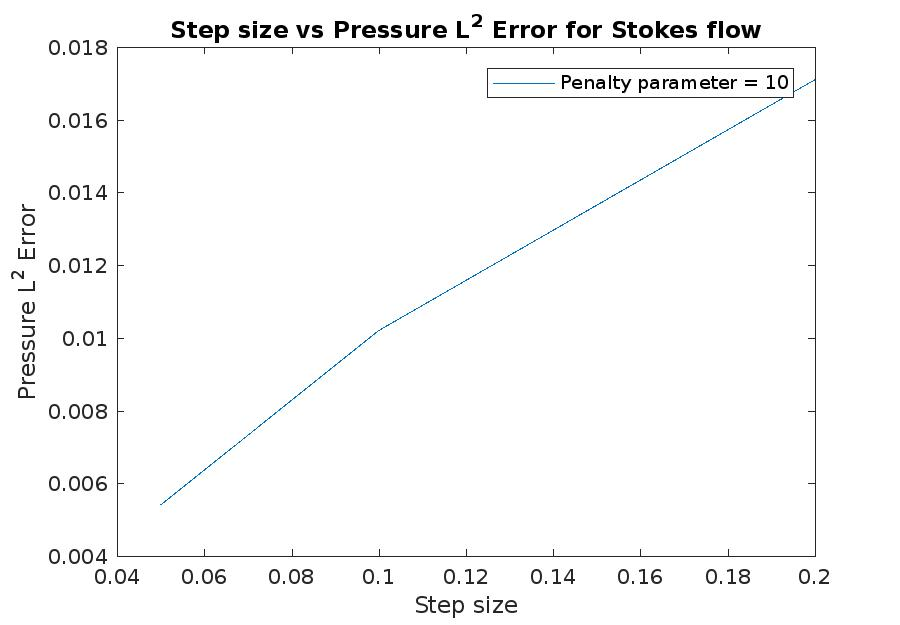
\includegraphics[width=\linewidth]{l2_pressure_stokes.jpg}
  \caption{$h-$ convergence test for pressure in $L^2$ error}
  \label{fig:pre_stoke_conv}
\end{subfigure}
\end{figure}
\begin{figure}
\begin{subfigure}{\textwidth}	
  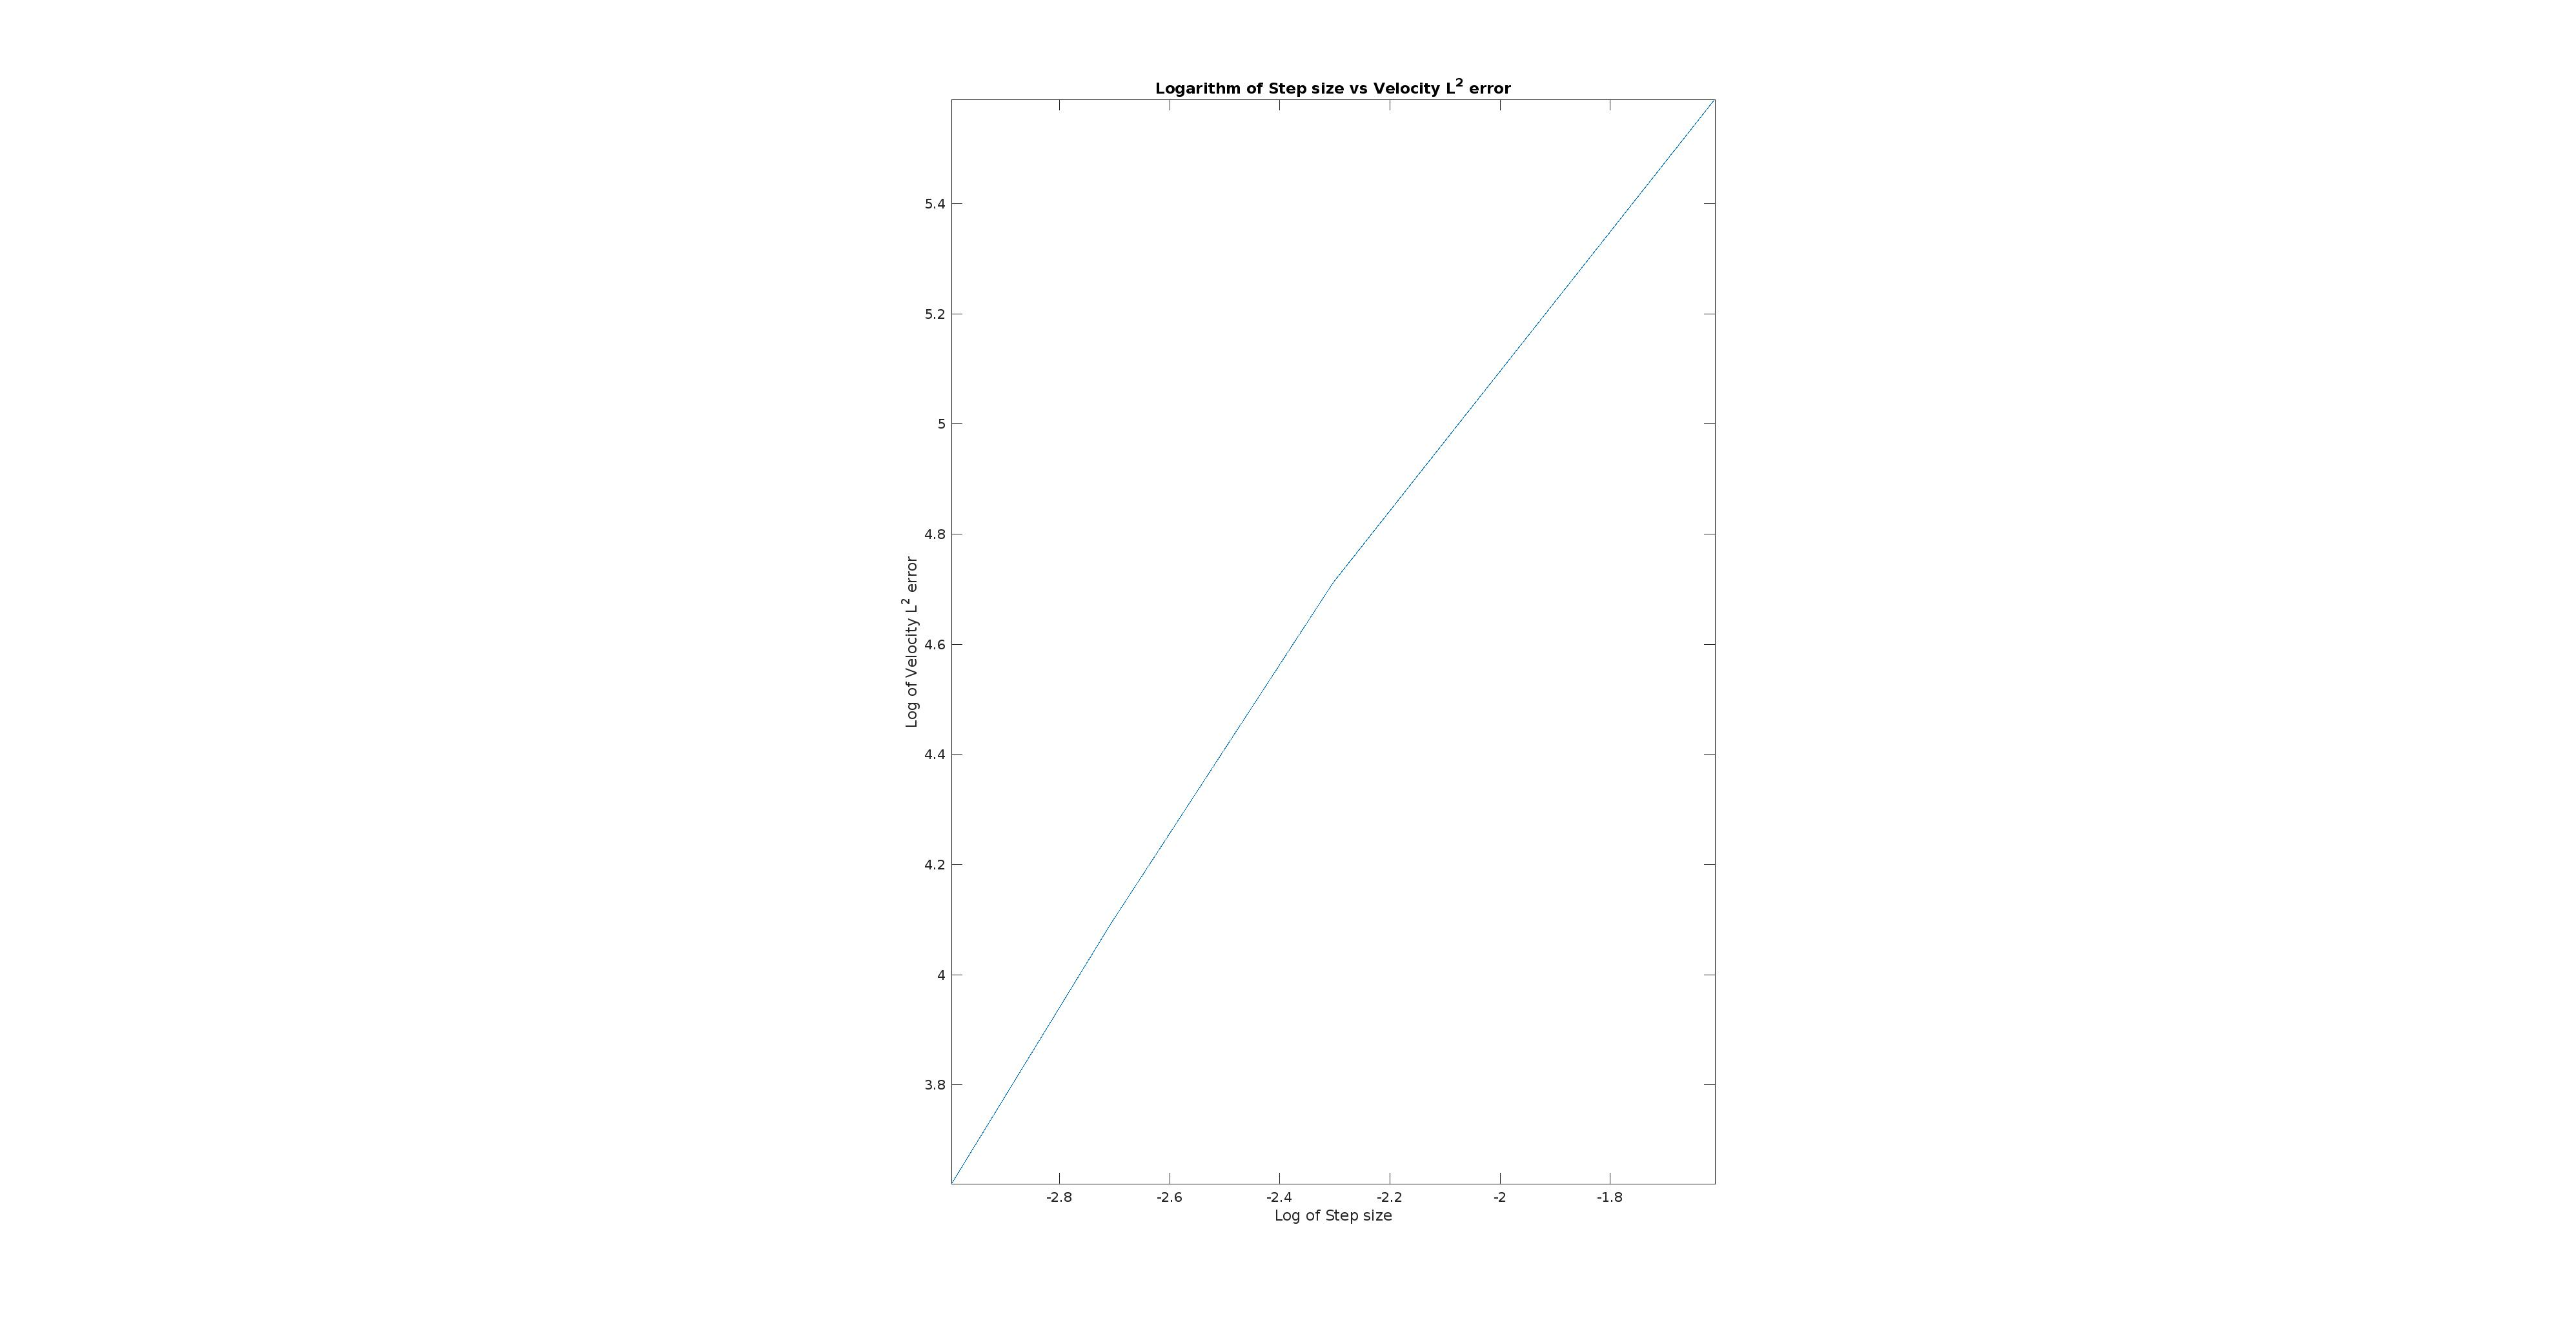
\includegraphics[width=\linewidth]{l2_velocity_log_stokes.jpg}
  \caption{$h-$ convergence test for velocity $L^2$ error (logarithmic scale)}
  \label{fig:vel_stoke_conv_log}
\end{subfigure}
\begin{subfigure}{\textwidth}	
  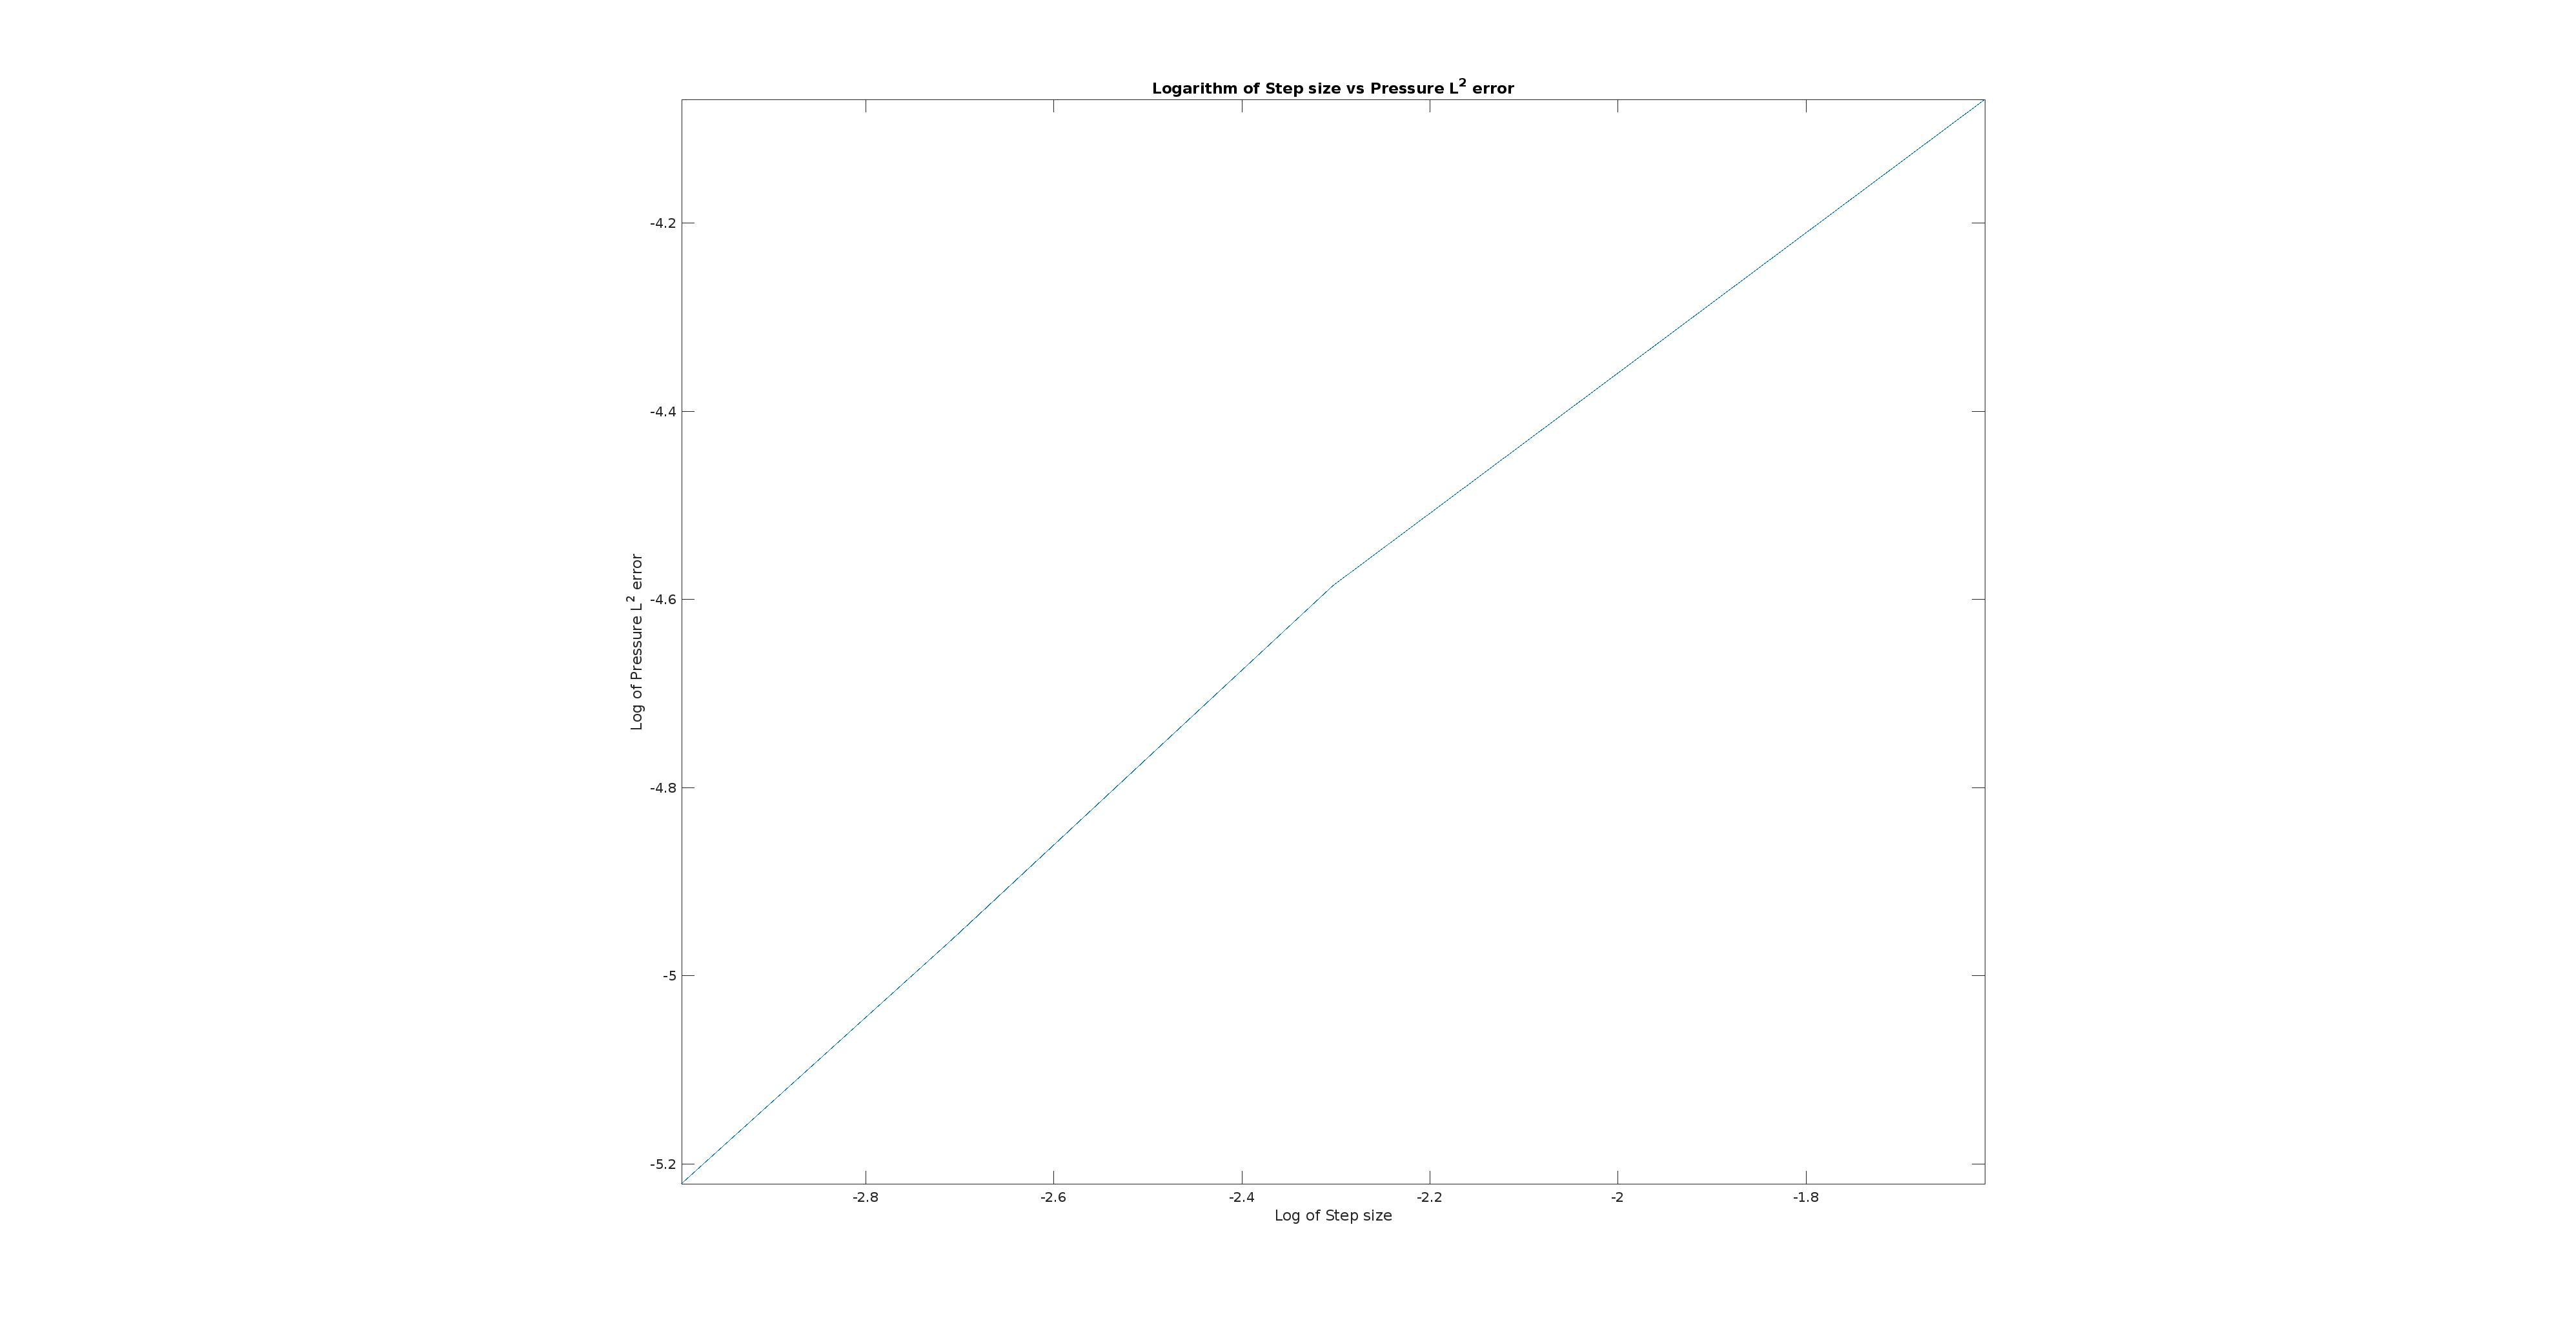
\includegraphics[width=\linewidth]{l2_pressure_log_stokes.jpg}
  \caption{$h-$ convergence test for pressure in $L^2$ error (logarithmic scale)}
  \label{fig:pre_stoke_conv_log}
\end{subfigure}
\label{fig:l2_stokes}
\end{figure}

\begin{figure}
\begin{subfigure}{\textwidth}	
  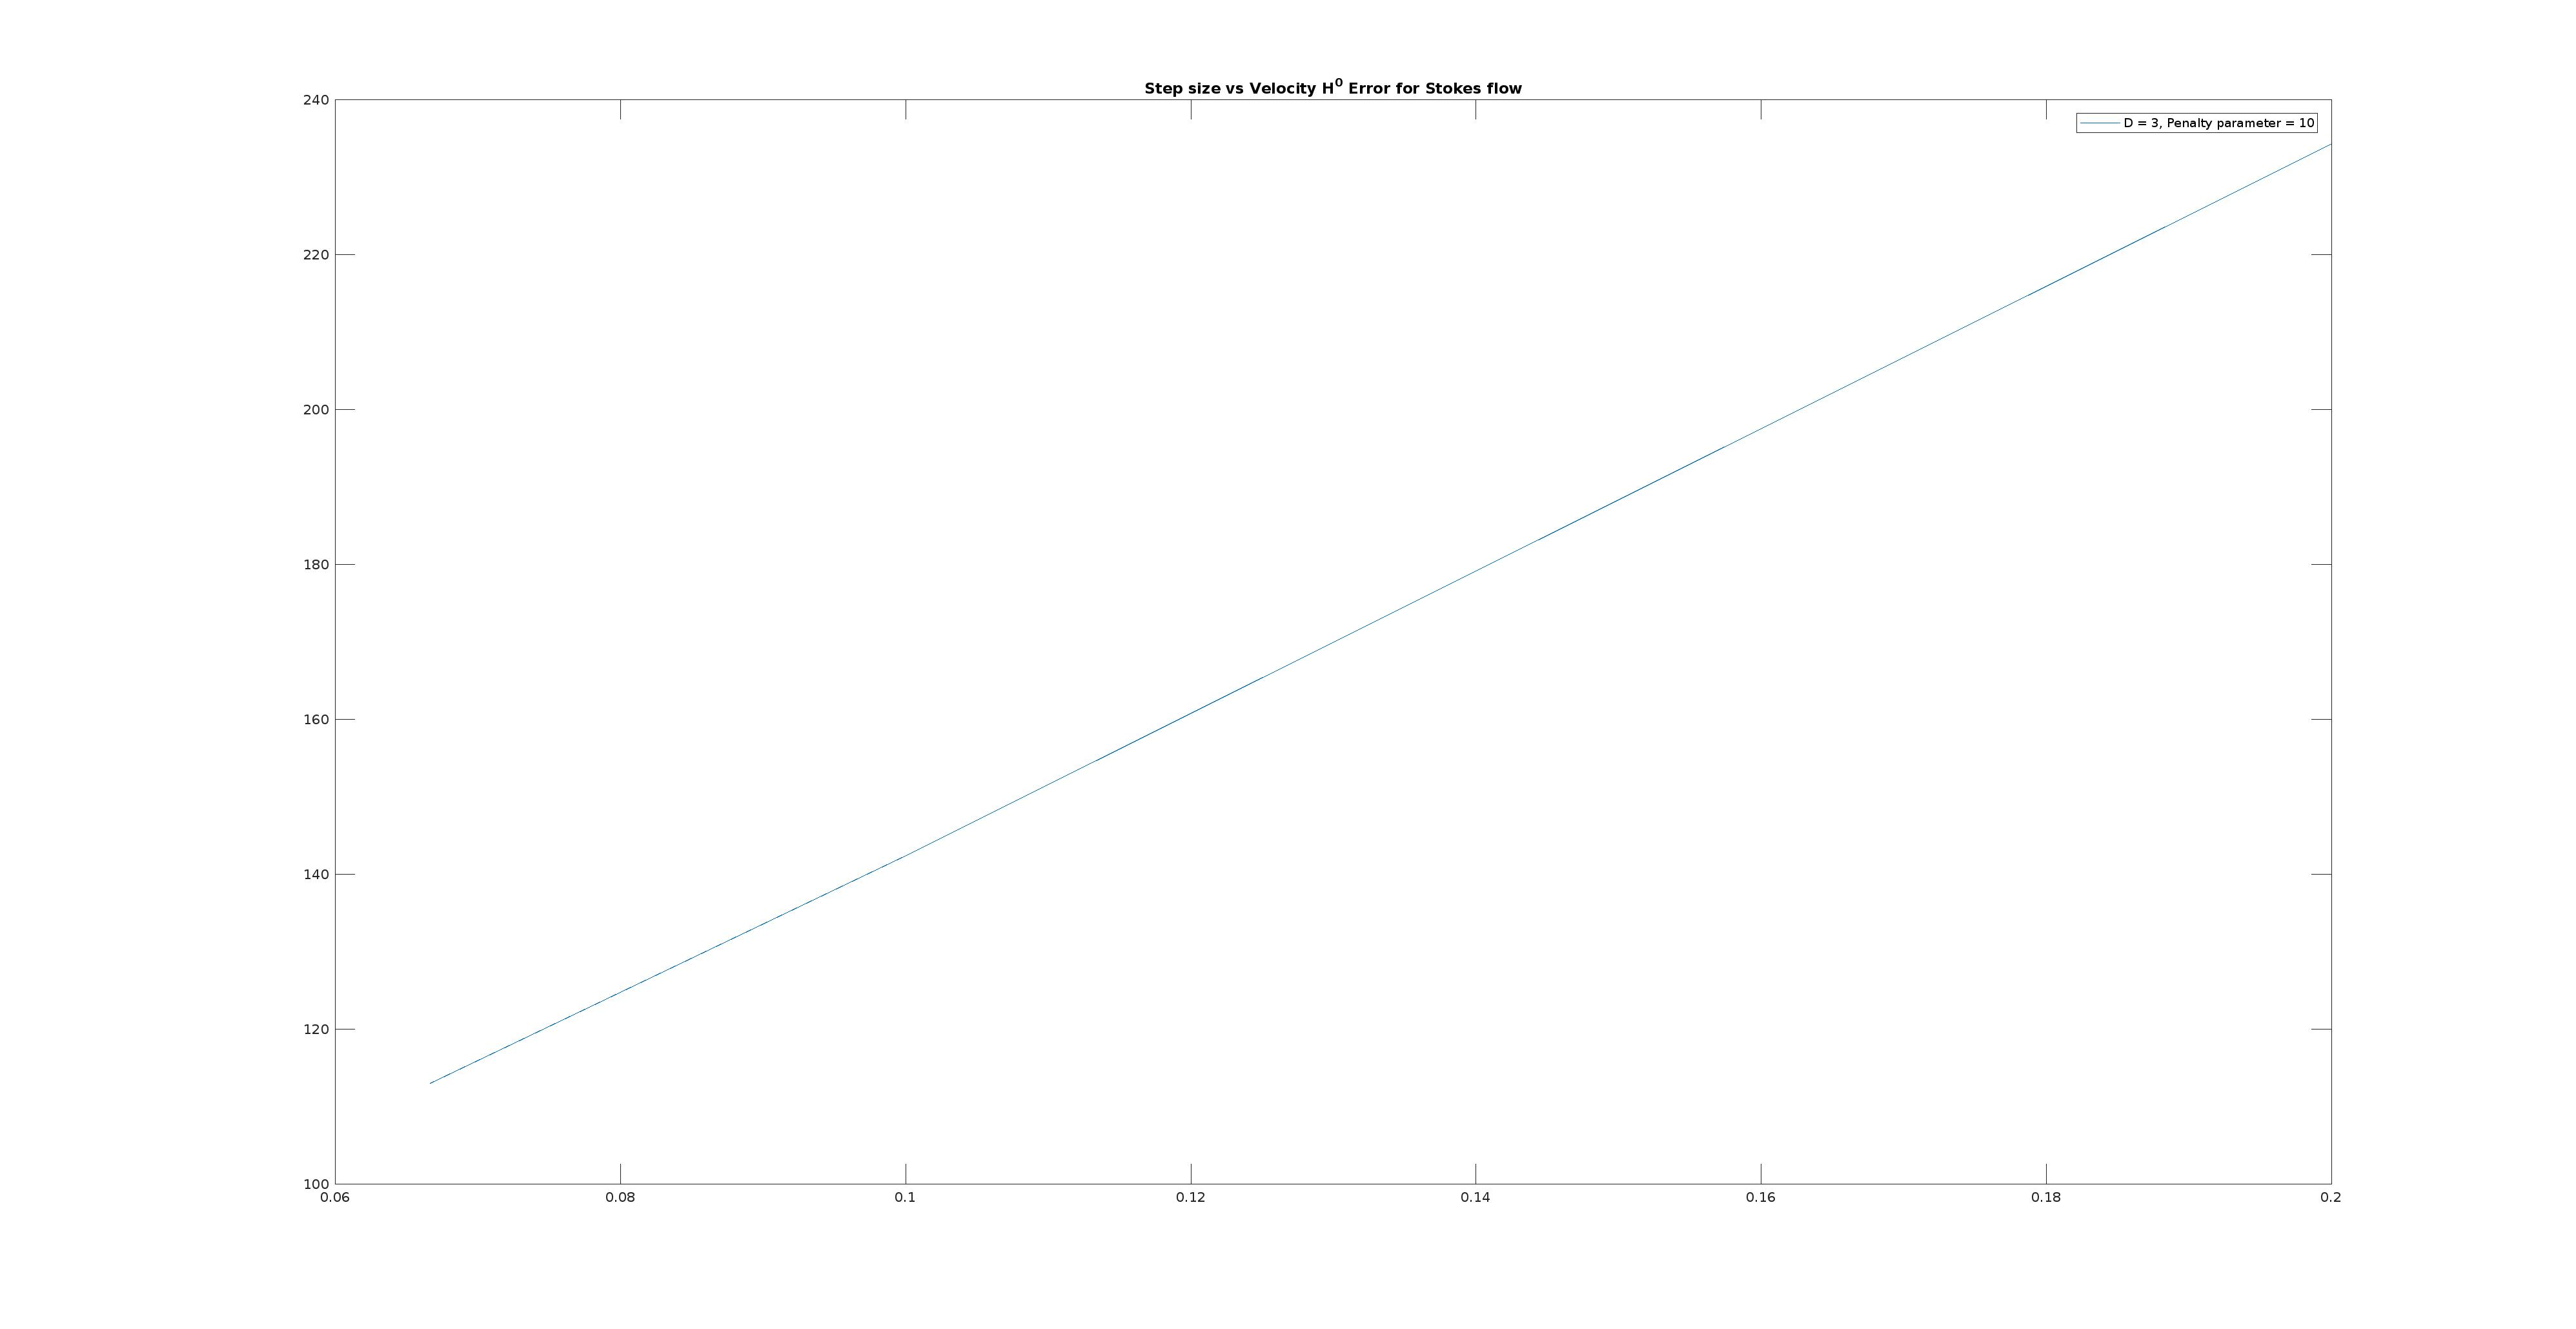
\includegraphics[width=\linewidth]{h0_velocity_stokes.jpg}
  \caption{$h-$ convergence test for velocity $H_0$ error}
  \label{fig:vel_stoke_conv_h0}
\end{subfigure}
\begin{subfigure}{\textwidth}	
  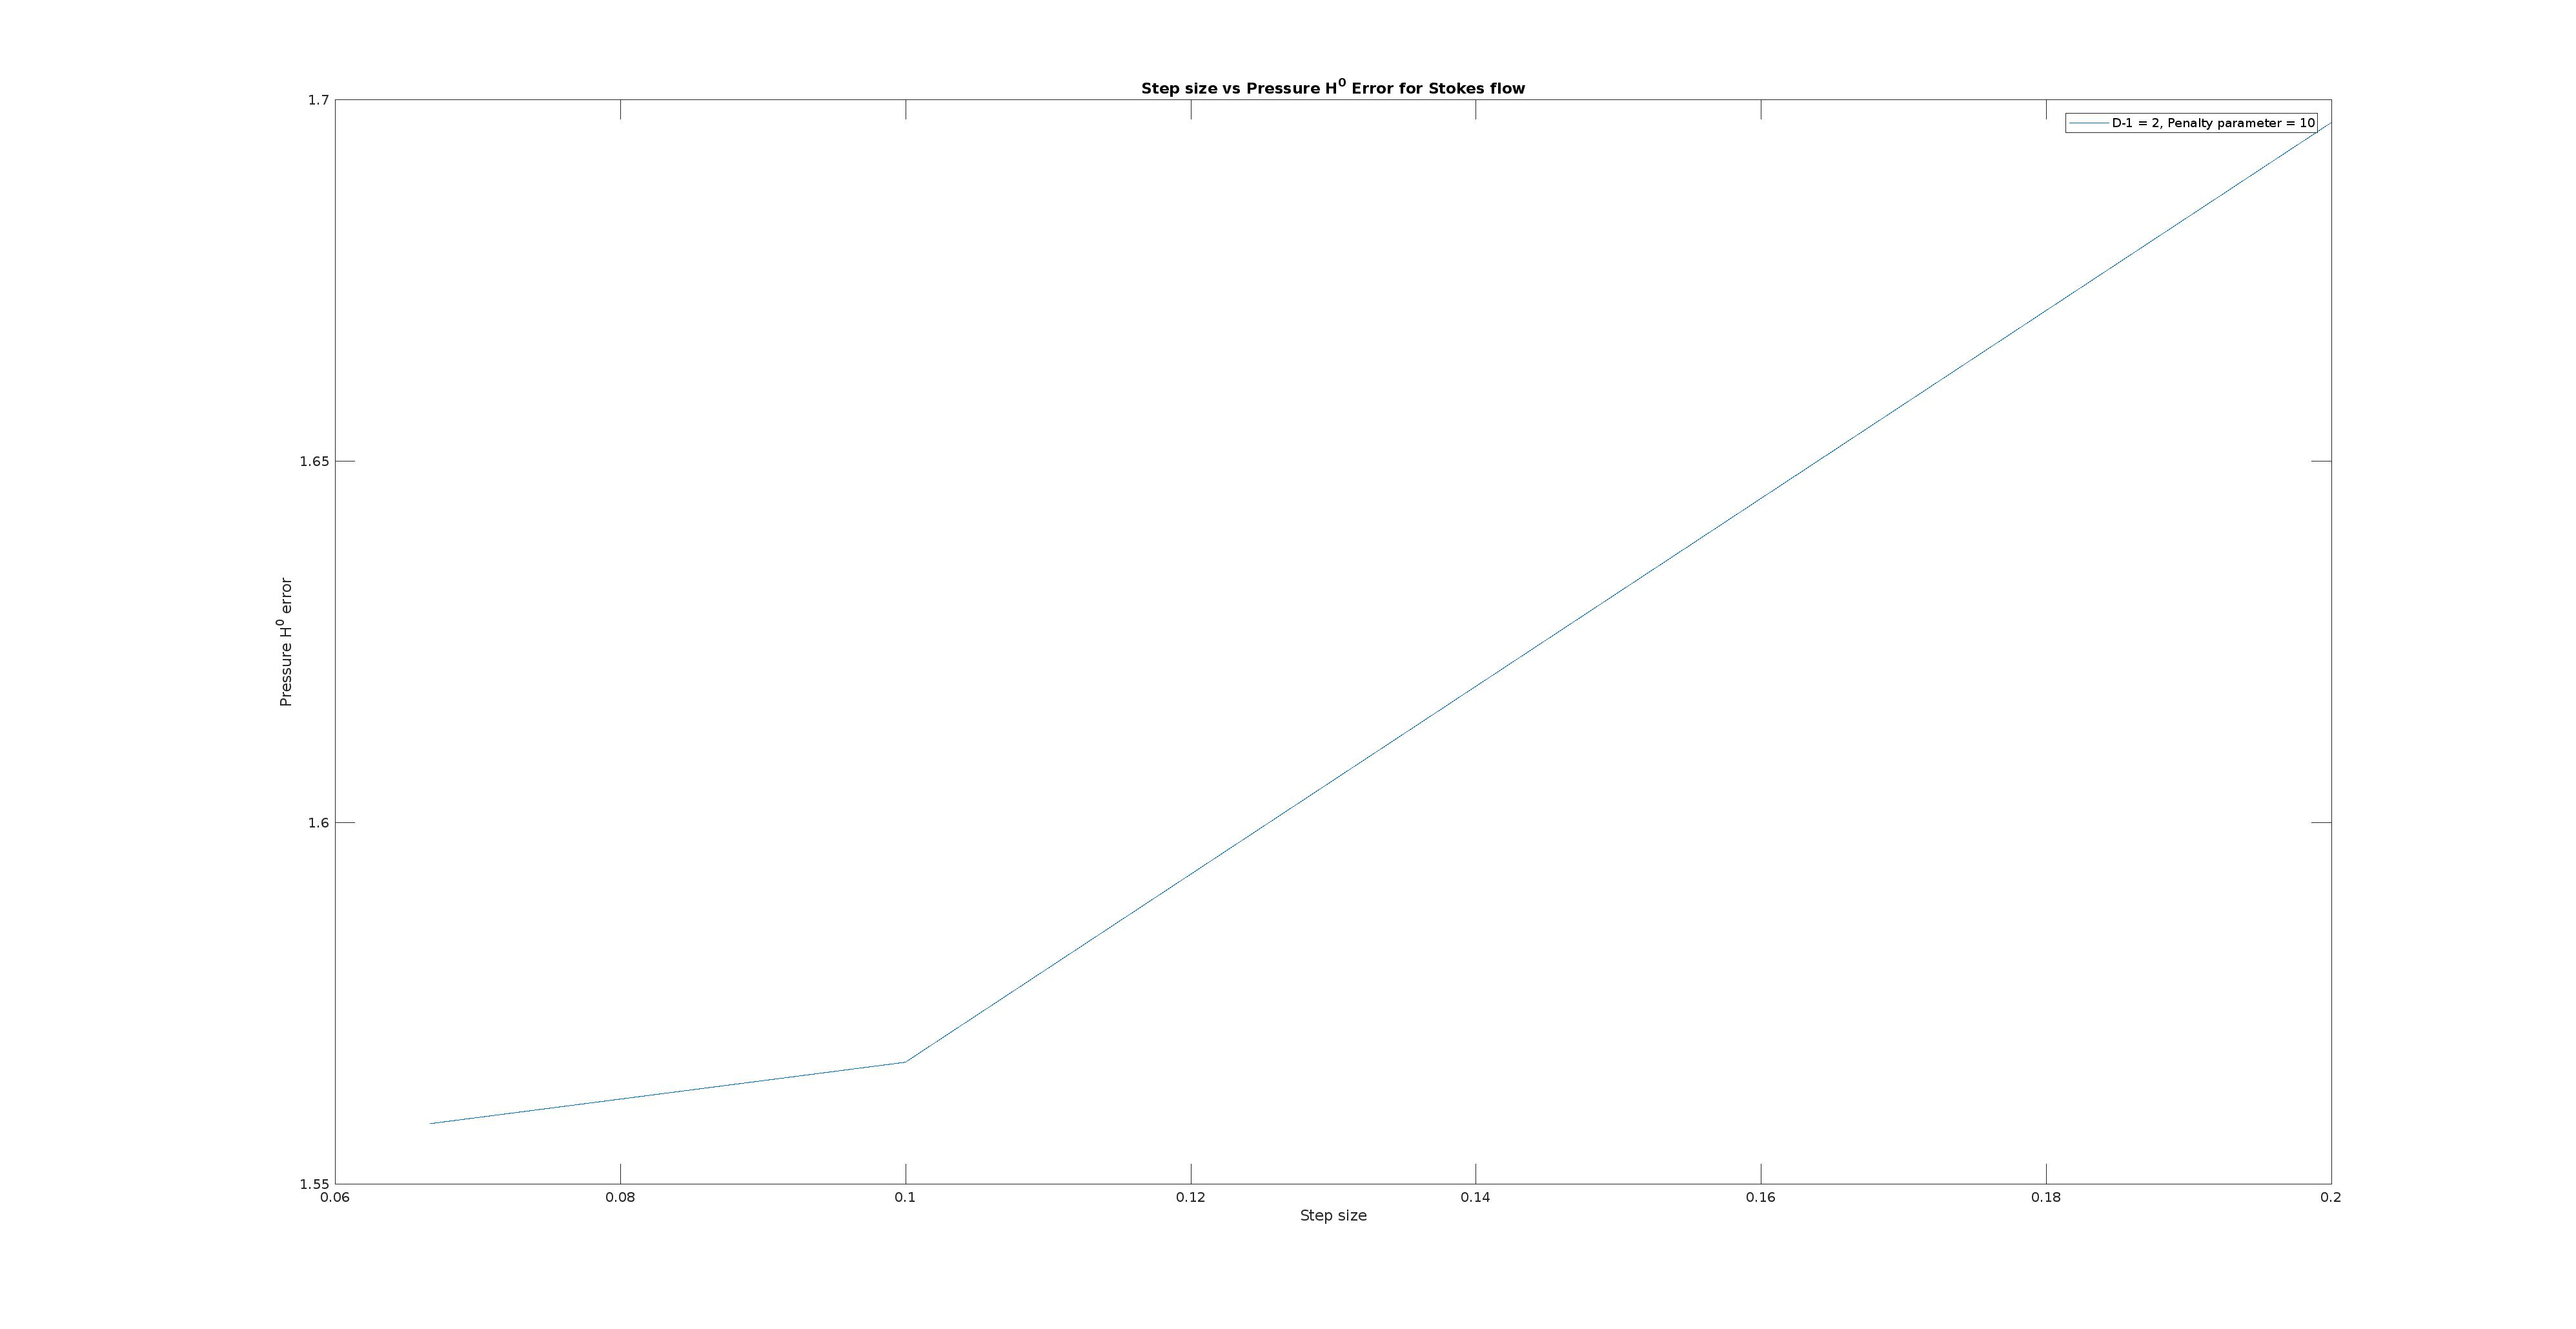
\includegraphics[width=\linewidth]{h0_pressure_stokes.jpg}
  \caption{$h-$ convergence test for pressure in $H_0$ error}
  \label{fig:pre_stoke_conv_h0}
\end{subfigure}
\end{figure}
\begin{figure}
\begin{subfigure}{\textwidth}	
  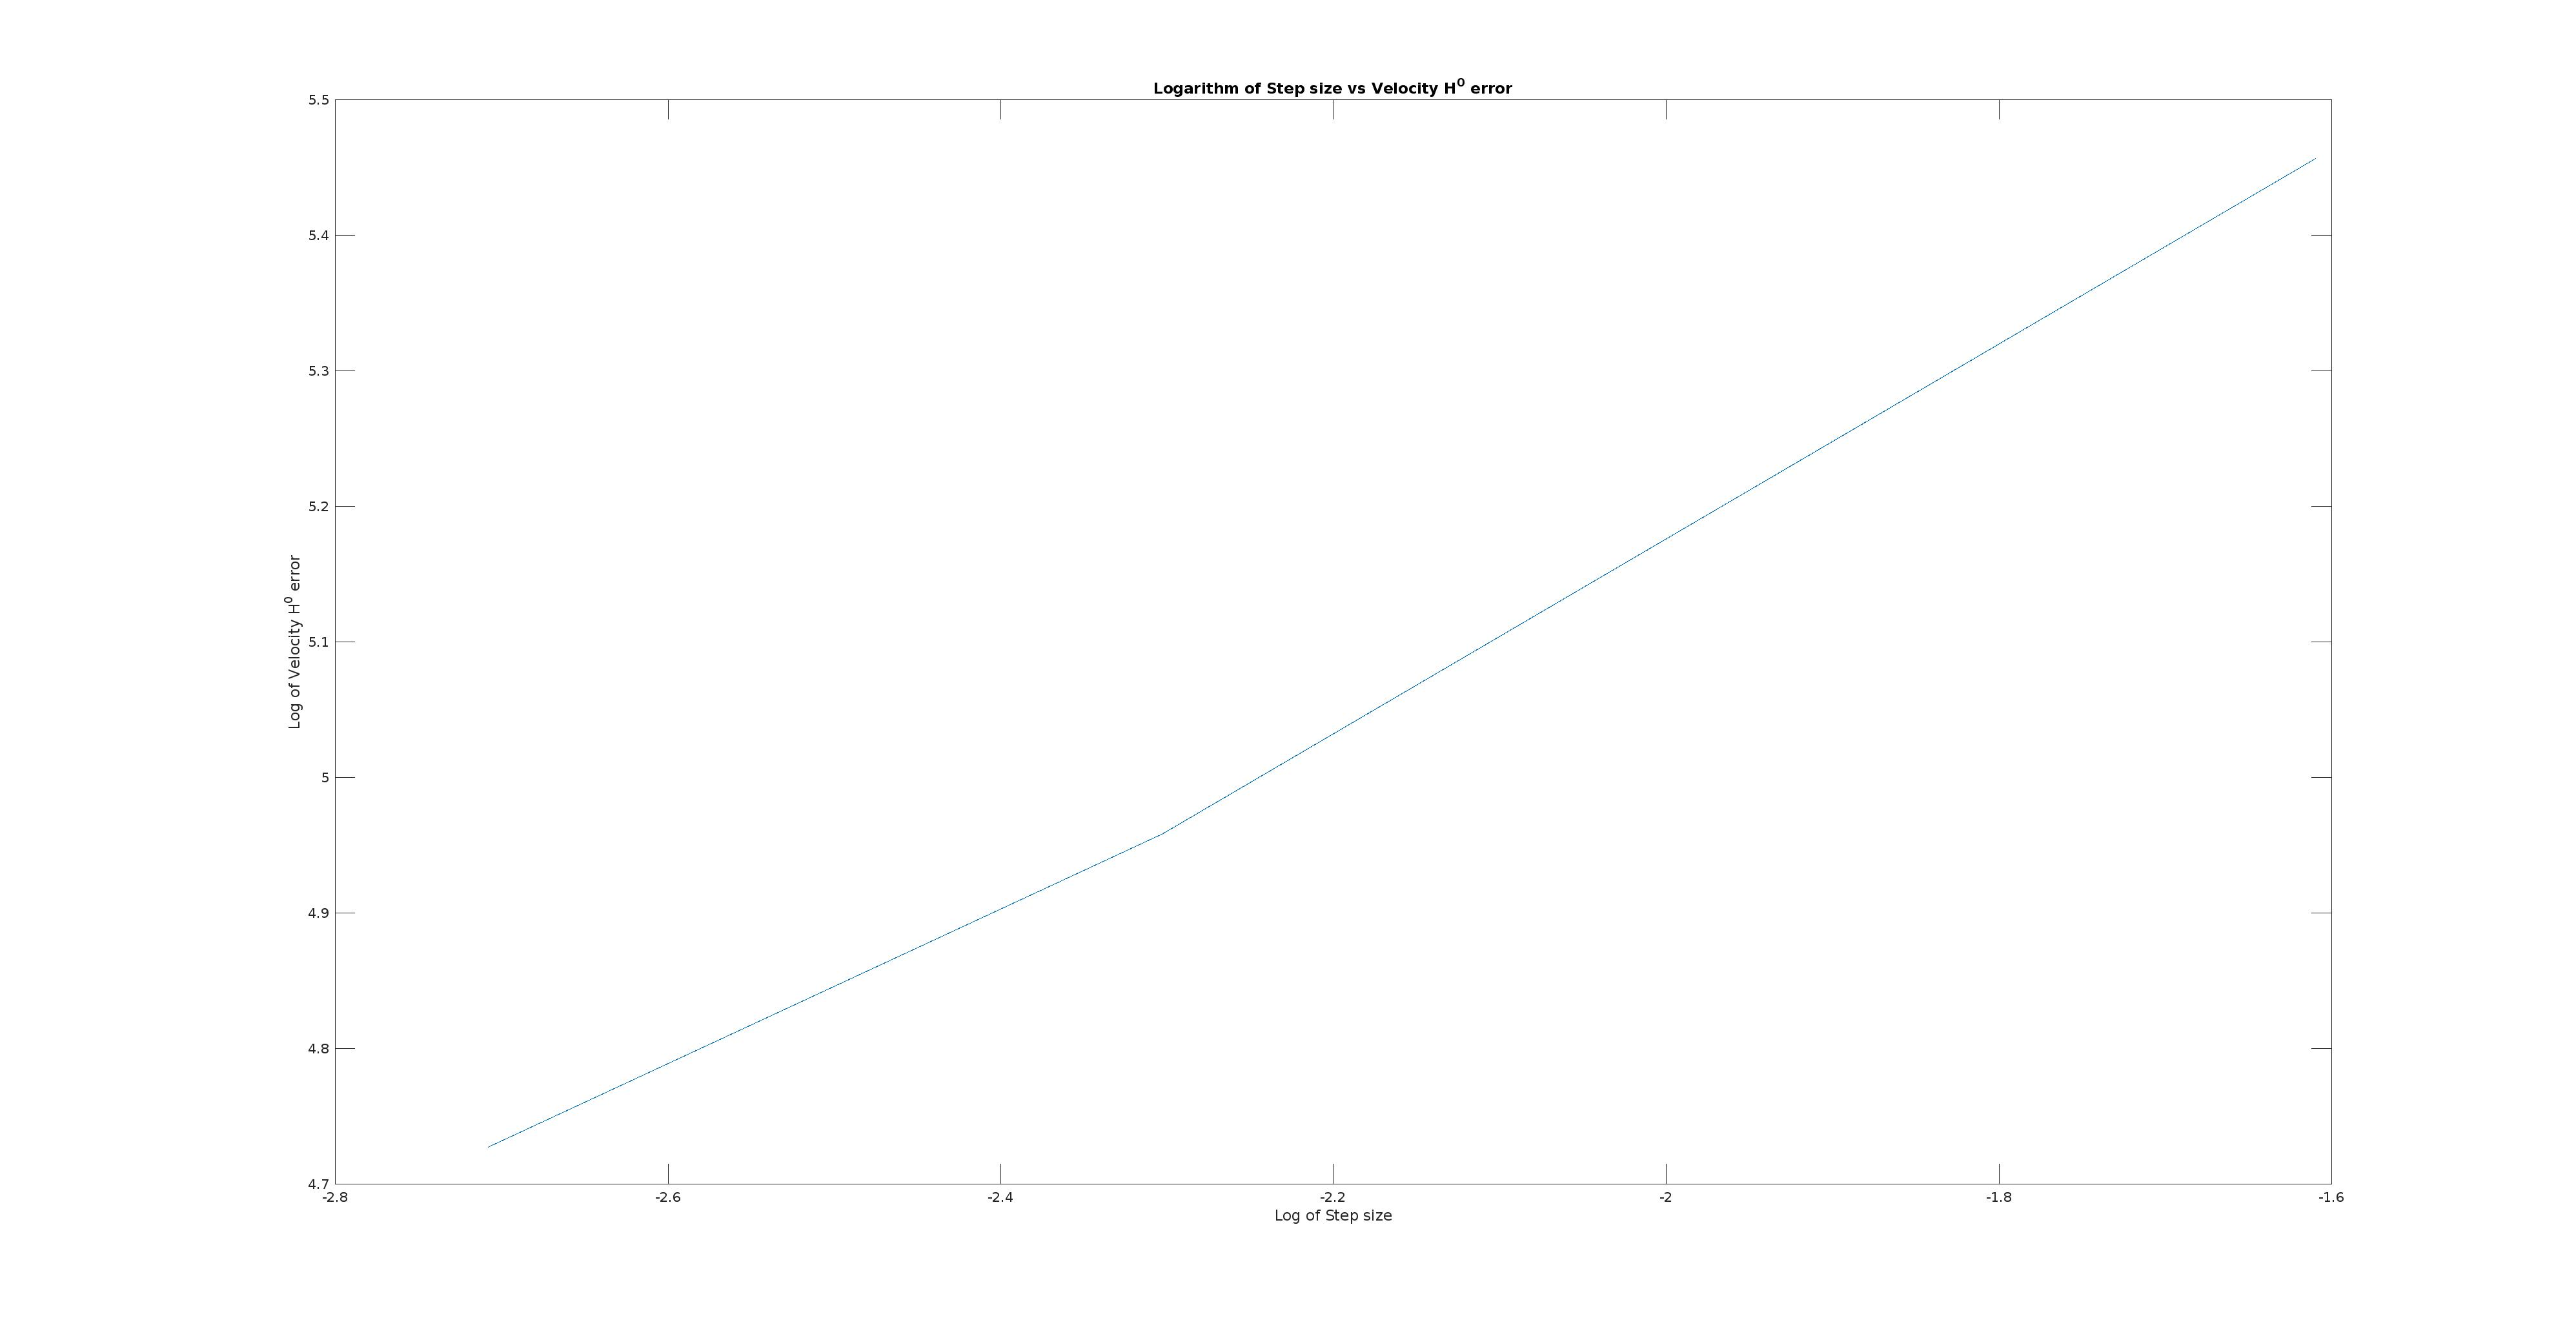
\includegraphics[width=\linewidth]{h0_velocity_log_stokes.jpg}
  \caption{$h-$ convergence test for velocity $H_0$ error (logarithmic scale)}
  \label{fig:vel_stoke_conv_log_h0}
\end{subfigure}
\begin{subfigure}{\textwidth}	
  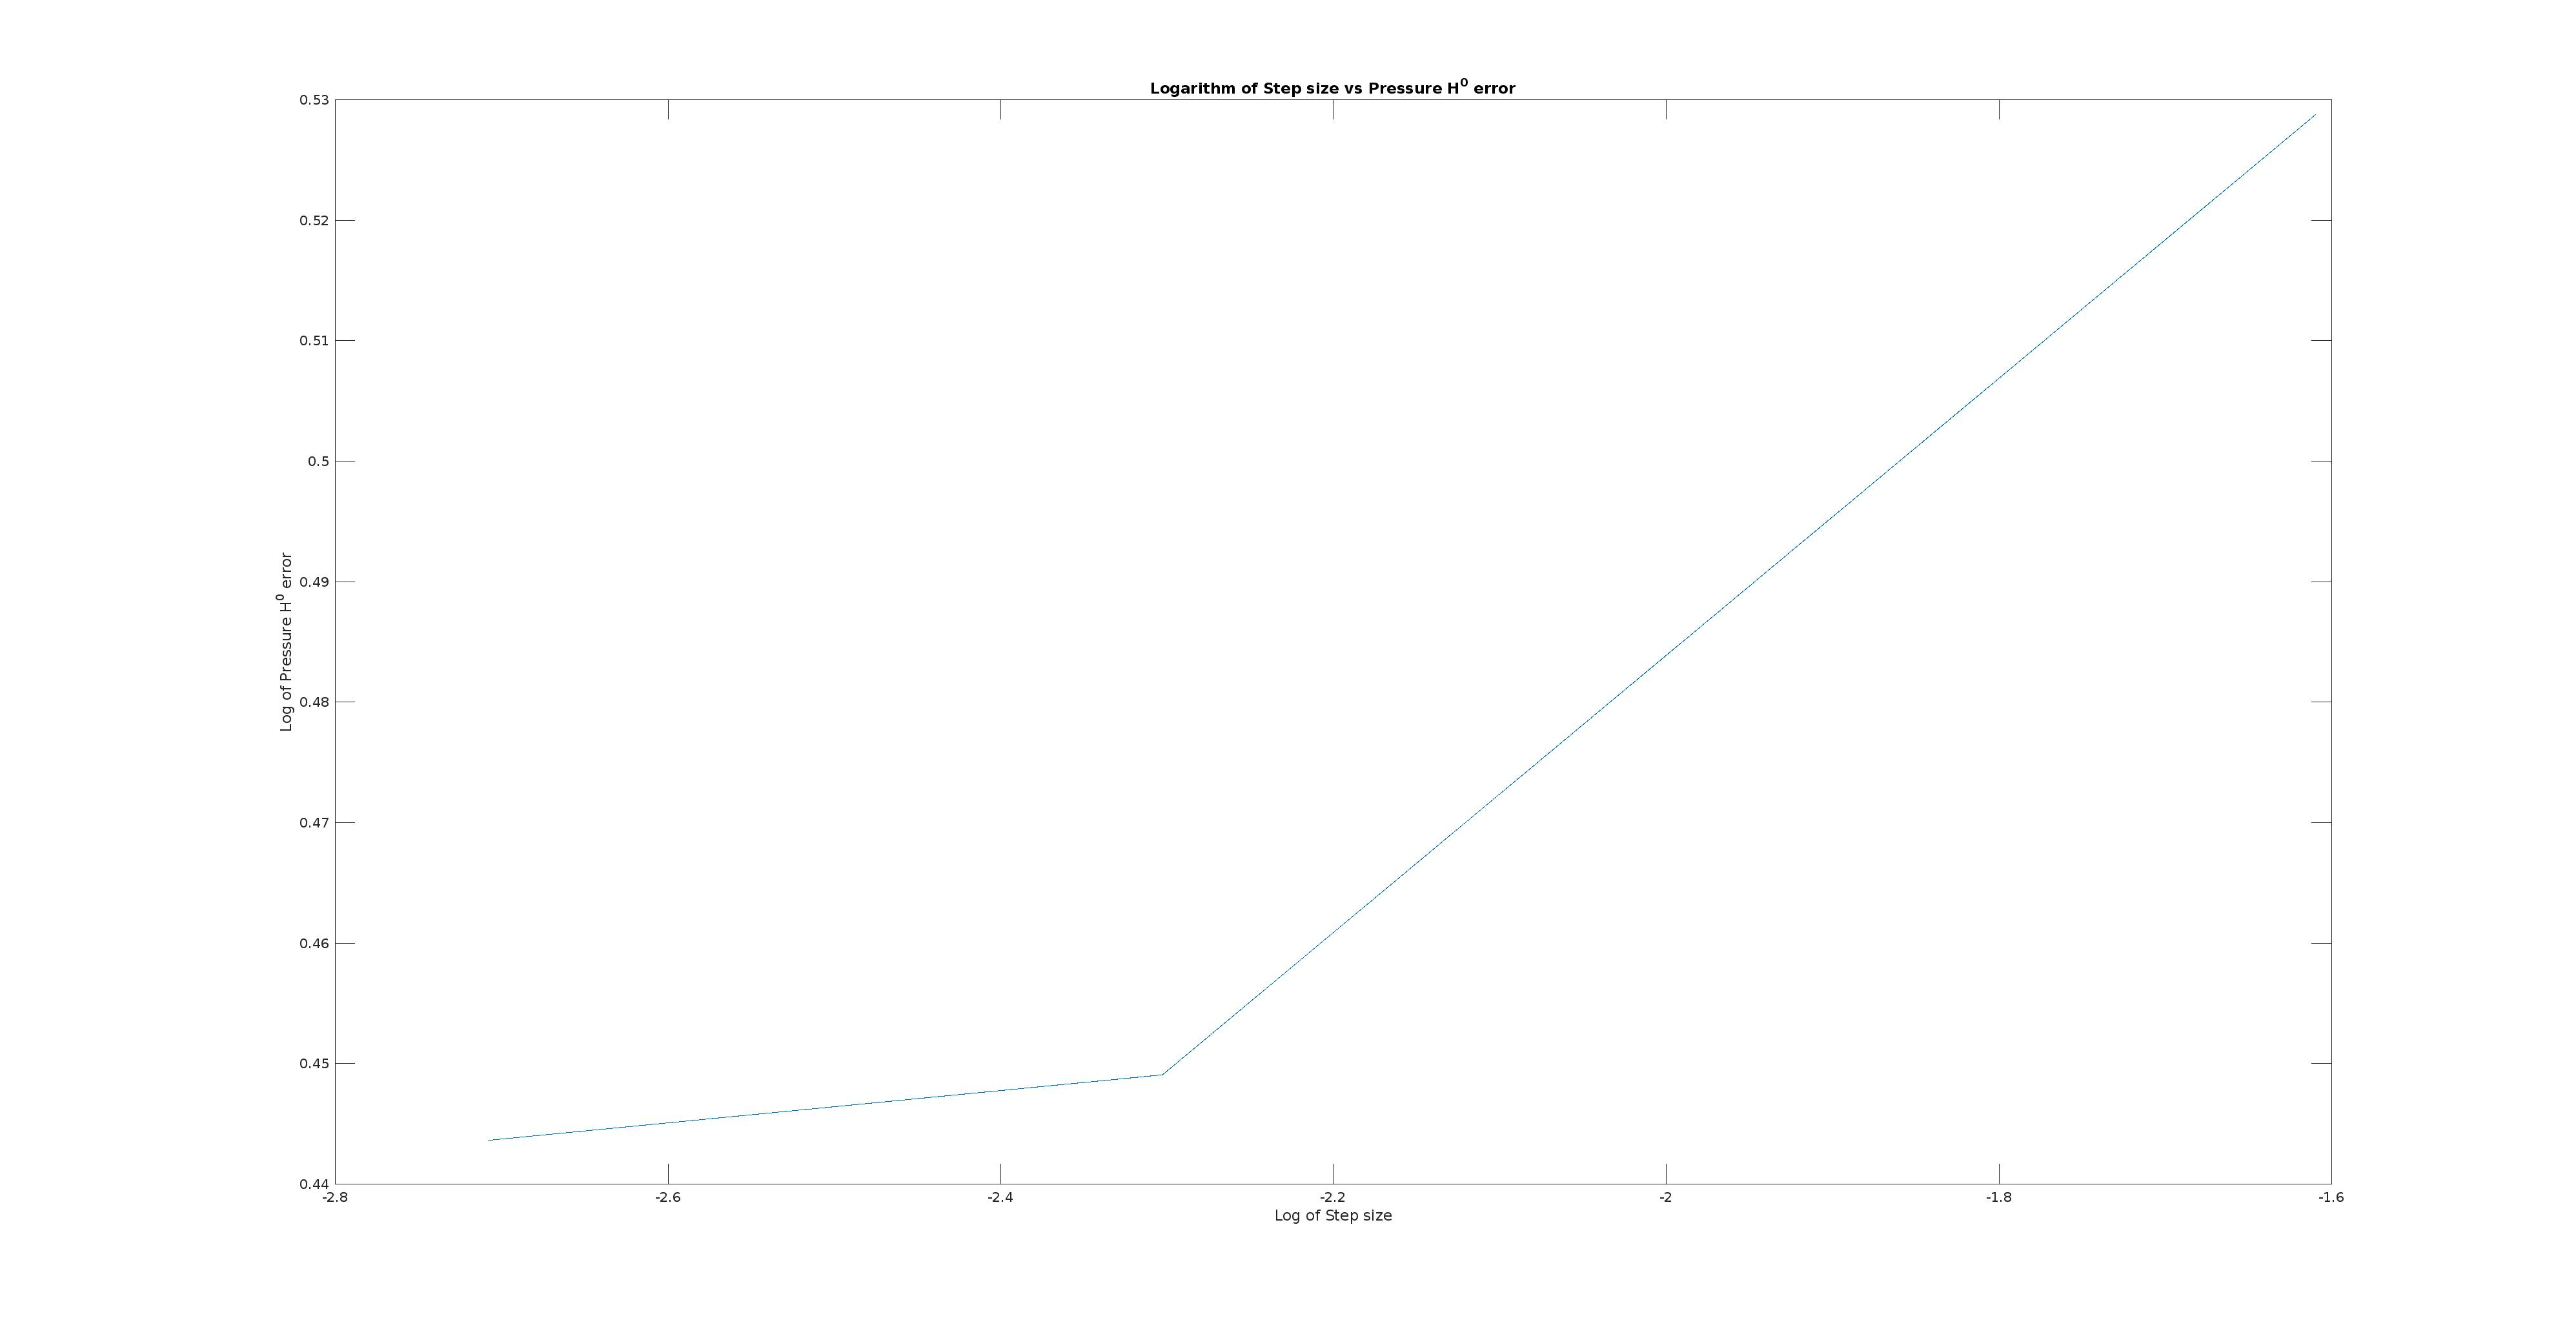
\includegraphics[width=\linewidth]{h0_pressure_log_stokes.jpg}
  \caption{$h-$ convergence test for pressure in $H_0$ error (logarithmic scale)}
  \label{fig:pre_stoke_conv_log_h0}
\end{subfigure}
\label{fig:h0_stokes}
\end{figure}

\begin{figure}
\begin{subfigure}{\textwidth}	
  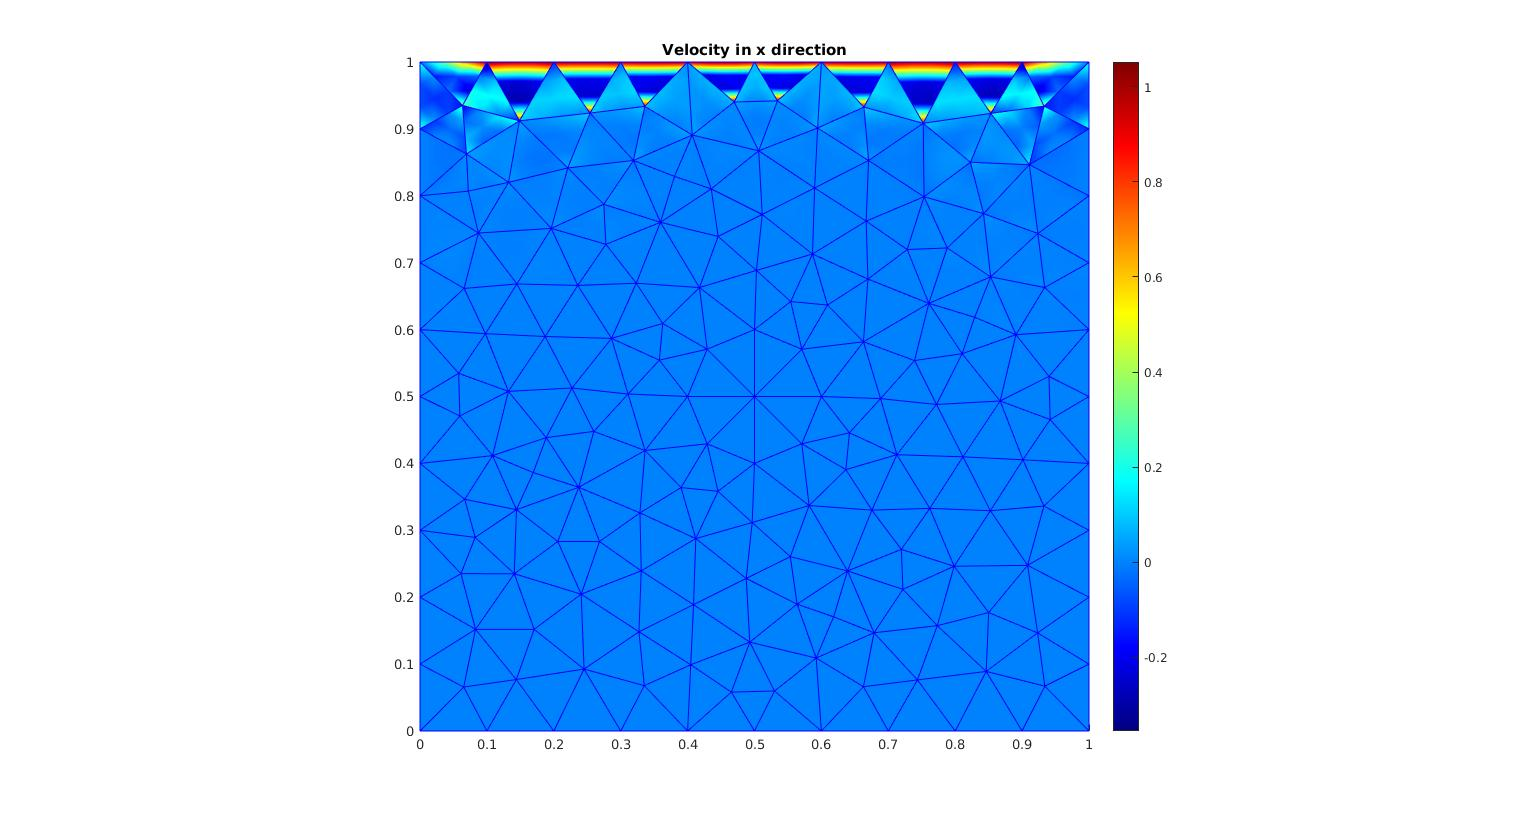
\includegraphics[width=\textwidth]{lid_bicgstab_vx.jpg}
  \caption{$x-$ velocity (bicgstab solver)} 
  \label{x_vel_stoke_bicgstab_lid}
\end{subfigure}
\begin{subfigure}{\textwidth}	
  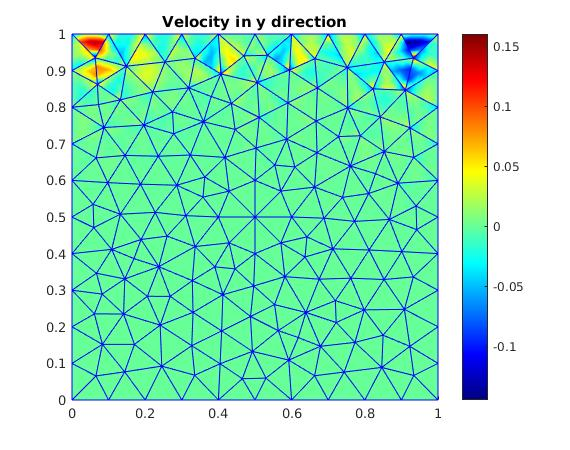
\includegraphics[width=\textwidth]{lid_bicgstab_vy.jpg}
  \caption{$y-$ velocity (bicgstab solver)} 
  \label{y_vel_stoke_bicgstab_lid}
\end{subfigure}
\begin{subfigure}{\textwidth}	
  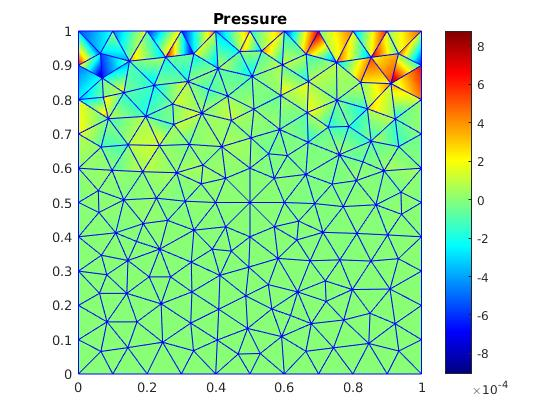
\includegraphics[width=\textwidth]{lid_bicgstab_pressure.jpg}
  \caption{Pressure (bicgstab solver)} 
  \label{pressure_stoke_bicgstab_lid}
\end{subfigure}
\caption{\label{stoke_bicgstab_lid}}
\end{figure}

\begin{figure}
\begin{subfigure}{\textwidth}	
  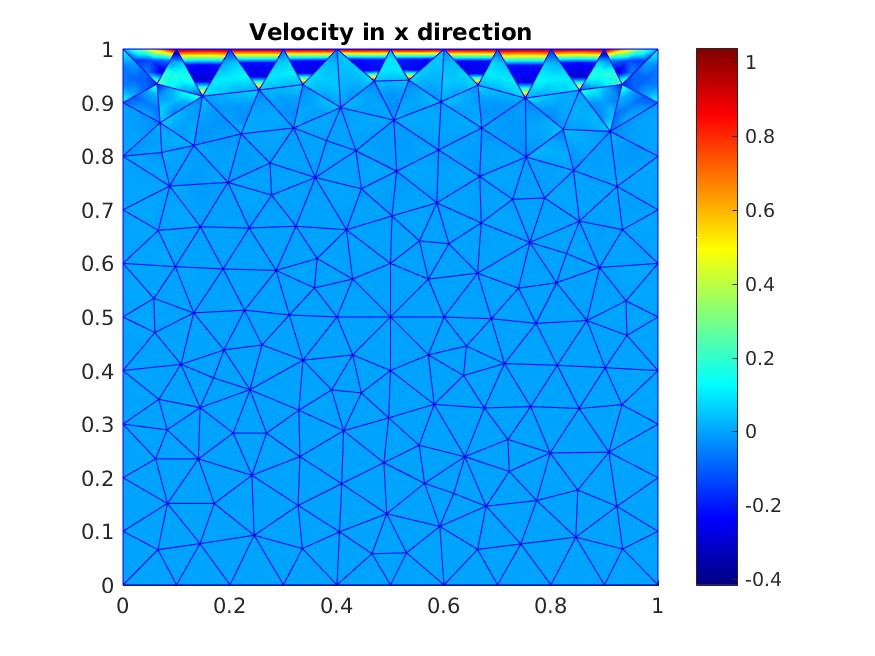
\includegraphics[width=\textwidth]{lid_minres_vx.jpg}
  \caption{$x-$ velocity (minres solver)} 
  \label{x_vel_stoke_minres_lid}
\end{subfigure}
\begin{subfigure}{\textwidth}	
  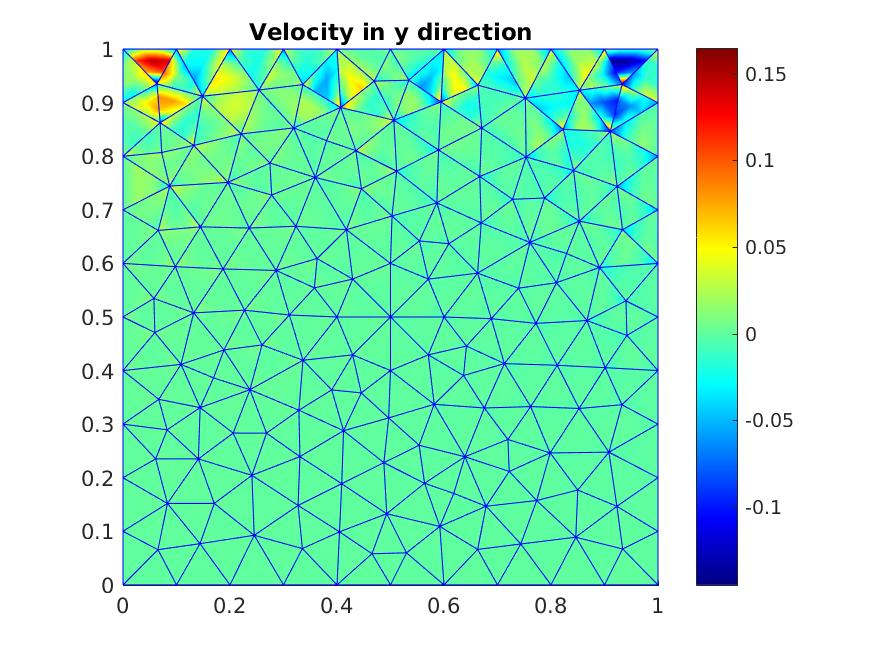
\includegraphics[width=\textwidth]{lid_minres_vy.jpg}
  \caption{$y-$ velocity (minres solver)} 
  \label{y_vel_stoke_minres_lid}
\end{subfigure}
\begin{subfigure}{\textwidth}	
  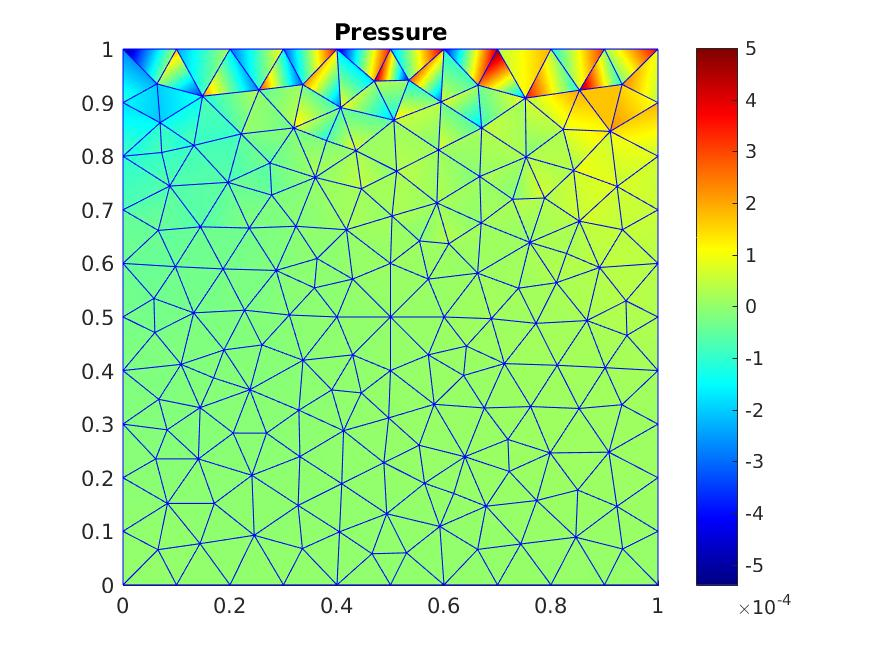
\includegraphics[width=\textwidth]{lid_minres_pressure.jpg}
  \caption{Pressure (minres solver)} 
  \label{pressure_stoke_minres_lid}
\end{subfigure}
\caption{\label{stoke_minres_lid}}
\end{figure}

\begin{figure}
\begin{subfigure}{\textwidth}	
  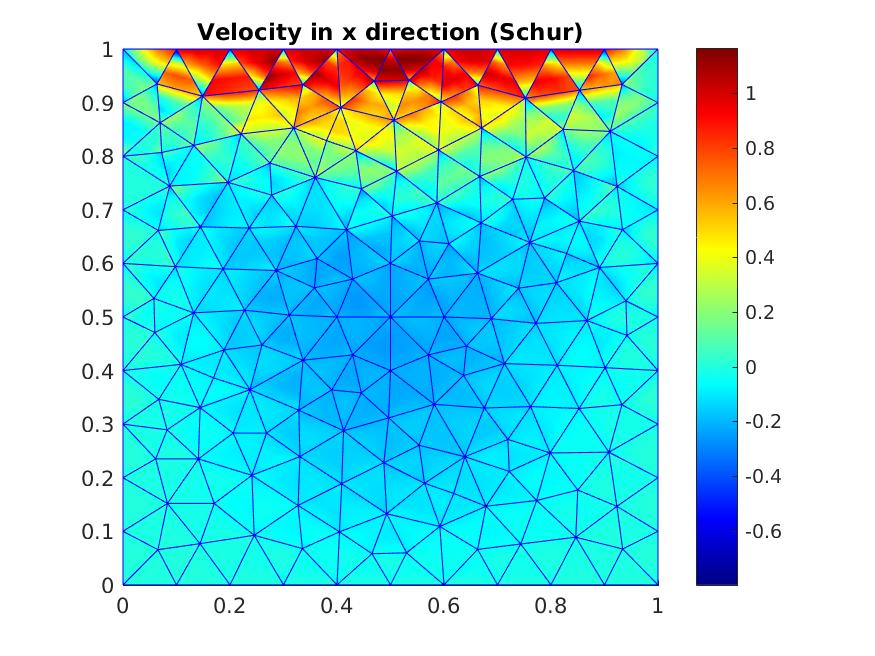
\includegraphics[width=\textwidth]{lid_schur_vx.jpg}
  \caption{$x-$ velocity (Schur complement method)} 
  \label{x_vel_stoke_schur_lid}
\end{subfigure}
\begin{subfigure}{\textwidth}	
  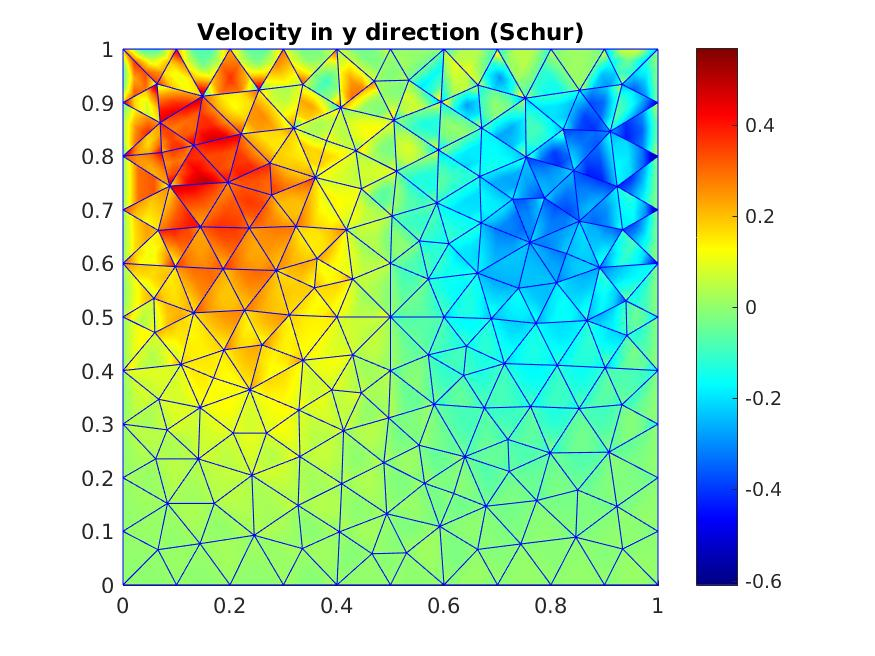
\includegraphics[width=\textwidth]{lid_schur_vy.jpg}
    \caption{$y-$ velocity (Schur complement method)} \label{y_vel_stoke_schur_lid}
\end{subfigure}
\begin{subfigure}{\textwidth}	
  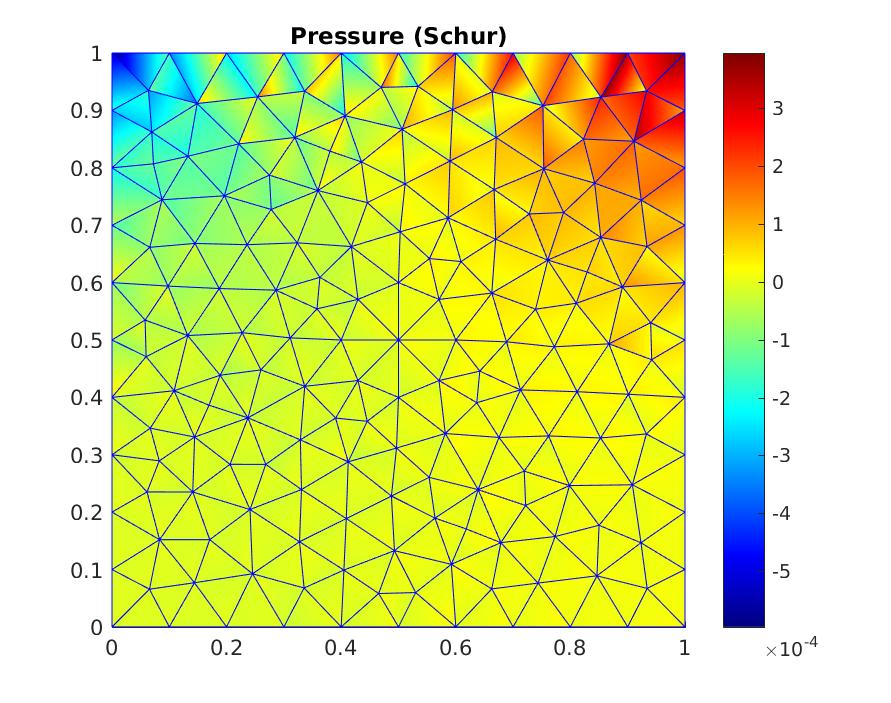
\includegraphics[width=\textwidth]{lid_schur_pressure.jpg}
    \caption{Pressure (Schur complement method)} 
    \label{pressure_stoke_schur_lid}
\end{subfigure}
\caption{\label{stoke_schur_lid}}
\end{figure}

\begin{figure}
\begin{subfigure}{\textwidth}	
  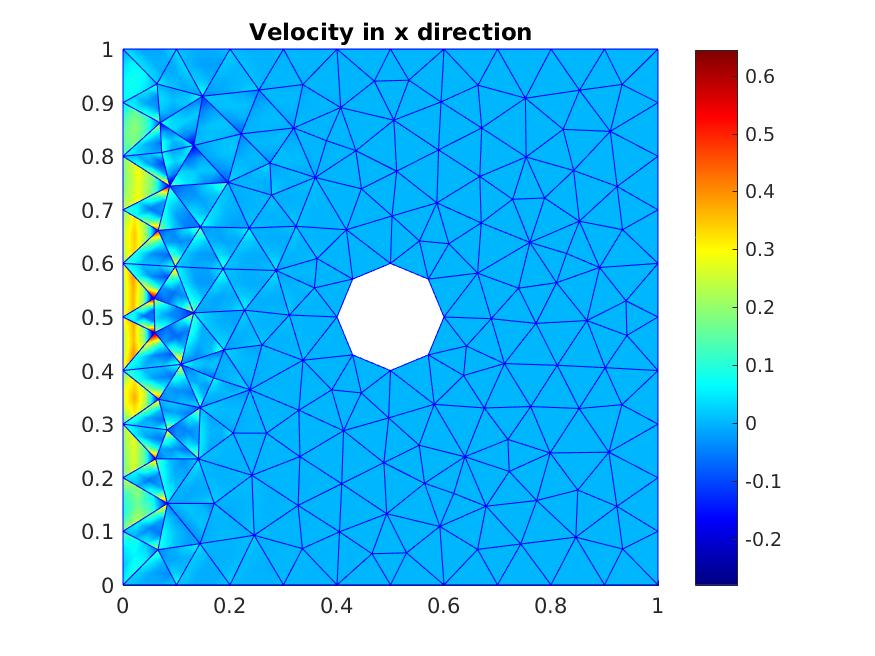
\includegraphics[width=\textwidth]{cylinder_bicgstab_vx.jpg}
      \caption{$x-$ velocity (bicgstab solver)}
    \label{x_vel_stoke_bicgstab}
\end{subfigure}
\begin{subfigure}{\textwidth}	
      \includegraphics[width=\textwidth]{cylinder_bicgstab_vy.jpg}
    \caption{$y-$ velocity (bicgstab solver)}
     \label{y_vel_stoke_bicgstab}
\end{subfigure}
\begin{subfigure}{\textwidth}	
    \includegraphics[width=\textwidth]{cylinder_bicgstab_pressure.jpg}
    \caption{Pressure (bicgstab solver)}
      \label{pressure_stoke_bicgstab}
\end{subfigure}
\caption{\label{flow_over_cylinder_bicgstab}}
\end{figure}

\begin{figure}
\begin{subfigure}{\textwidth}	
  \includegraphics[width=\textwidth]{cylinder_minres_vx.jpg}
    \caption{$x-$ velocity (minres solver)}
    \label{x_vel_stoke_minres}
\end{subfigure}
\begin{subfigure}{\textwidth}	
    \includegraphics[width=\textwidth]{cylinder_minres_vy.jpg}
    \caption{$y-$ velocity (minres solver)}
     \label{y_vel_stoke_minres}
\end{subfigure}
\begin{subfigure}{\textwidth}	
    \includegraphics[width=\textwidth]{cylinder_minres_pressure.jpg}
    \caption{Pressure (minres solver)}
      \label{pressure_stoke_minres}
\end{subfigure}
\caption{\label{flow_over_cylinder_minres}}
\end{figure}

\begin{figure}
\begin{subfigure}{\textwidth}	
    \includegraphics[width=\textwidth]{cylinder_schur_vx.jpg}
    \caption{$x-$ velocity (Schur complement method)}
    \label{x_vel_stoke_schur}
\end{subfigure}
\begin{subfigure}{\textwidth}	
    \includegraphics[width=\textwidth]{cylinder_schur_vy.jpg}
    \caption{$y-$ velocity (Schur complement method)}
     \label{y_vel_stoke_schur}
\end{subfigure}
\begin{subfigure}{\textwidth}	
    \includegraphics[width=\textwidth]{cylinder_schur_pressure.jpg}
    \caption{Pressure (Schur complement method)}
      \label{pressure_stoke_schur}
\end{subfigure}
\caption{\label{flow_over_cylinder_schur}}
\end{figure}

\section{Penalty parameter}

We now measure the effect of the penalty parameter on the condition number of the matrix $A$. While coercivity provides a lower limit for the penalty parameter, the upper limit is based on an affordable condition number of the matrix $A$. As shown in Figure \ref{penalty_condition_number}, the condition number of the matrix $A$ increases with increasing penalty parameter.
The condition number is measured on a unit square [0,1] $\times$ [0,1] in the $x-y$ plane with the number of intervals $10 \times 10$. The penalty parameter ranged from $1e \minus 2$ to $1e4$. The corresponding condition number ranged from $3.750e5$ to $1.445e10$. We see a linear increase in the condition number of the stiffness matrix with respect to the penalty parameter. (Figure \ref{effect_penalty_parameter}) The linear increase is in agreement with results of Montlaur et al. \cite{Montlaur}.

We also solve flow over cylinder problem from Section \ref{flow_over_cylinder_stokes} with penalty parameter smaller than required to maintain coercivity. The results as can be seen in Figure \ref{flow_over_cylinder_c11_low} is unable to produce physically relevant flow profile.

\begin{figure}
\begin{subfigure}{\textwidth}	
  \includegraphics[width=\linewidth]{grid_penalty_parameter.jpg}
  \caption{Unit square with $10 \times 10$ discretisation}
  \label{grid_penalty_para}
\end{subfigure}
\begin{subfigure}{\textwidth}	
	\includegraphics[width=\linewidth]{penalty_condition_number.jpg}
	\caption{Penalty parameter vs Condition number}
	\label{penalty_condition_number}
\end{subfigure}
\caption{\label{effect_penalty_parameter}}
\end{figure}

\begin{figure}
\begin{subfigure}{\textwidth}	
    \includegraphics[width=\textwidth]{c11_unphysical_vx.jpg}
    \caption{$x-$ velocity with penalty parameter smaller than minimum required for coercivity}
    \label{x_vel_stoke_c11_low}
\end{subfigure}
\begin{subfigure}{\textwidth}	
    \includegraphics[width=\textwidth]{c11_unphysical_vy.jpg}
    \caption{$y-$ velocity with penalty parameter smaller than minimum required for coercivity}
     \label{y_vel_stoke_c11_low}
\end{subfigure}
\begin{subfigure}{\textwidth}	
    \includegraphics[width=\textwidth]{c11_unphysical_pressure.jpg}
    \caption{Pressure with penalty parameter smaller than minimum required for coercivity}
      \label{pressure_stoke_c11_low}
\end{subfigure}
\caption{\label{flow_over_cylinder_c11_low}}
\end{figure}

\section{Navier Stokes flow}\label{N-S-ch5}

We recall that we use the initial guess from the Stokes equation and the Newton method presented in the Section  \ref{newton_method}. We also note that the stiffness matrix in case of the Navier Stokes equation is non symmetric and therefore, solvers applicable only for symmetric matrices can not be used. 

\subsection{Analytical example}

We now present an analytical example from \cite{Montlaur}. The domain considered for this example is the unit square $[0,1] \times [0,1]$ in the $x-y$ plane. 
The boundary ${x=0}$ is Dirichlet boundary with inflow velocity at point $(0,y)$ as $u = (0, 0)$. The boundaries ${x = 1}$, ${y = 0}$ and ${y = 1}$ are Dirichlet boundaries with no slip or zero velocity condition. The boundary ${x = 0}$ is a Neumann boundary with zero Neumann value i.e. $t = (0, 0)$. The source term is,

\begin{equation}
\begin{split}
f = (-4 \nu (1+2y) (y^2 - 6xy^2 + 6x^2 y^2 - y + 6xy \\ - 6x^2 y + 3x^2 - 6x^3 + 3x^4)+ 1 - 2x \\+ 4x^3 y^2 (2y^2 - 2y + 1)(y - 1)^2 (-1 + 2x)(x - 1)^3,\\ 4 \nu (-1 + 2x)(x^2 - 6x^2 y + 6x^2 y^2 - x + 6xy \\ - 6xy^2 + 3y^2 - 6y^3 + 3y^4) + \\ 4x^2y^3 (-1+2y)(y-1)^3 (2x^2-2x+1)(x-1)^2) \quad \textrm{.}
\end{split}
\end{equation}
 
The analytical solution for pressure and velocity reads as,

\begin{center}
\begin{equation}
p = x(1 - x)
\end{equation}
\begin{equation} 
\begin{split}
u = (x^2(1-y)^2(2y-6y^2+4y^3),\\-y^2(1-y)^2(2x-6x^2+4x^3)) \quad \textrm{.}
\end{split}
\end{equation}
\end{center}

The results of an $h-$convergence test in the $L^2$ norm is presented in Figures \ref{navier_stoke_conv_l2}, \ref{navier_stoke_conv_l2_log} and in the $H_0$ semi norm is presented in Figures \ref{navier_stoke_conv_h0}, \ref{navier_stoke_conv_h0_log}. The $L^2$ error results are found to be in agreement with Montlaur et al. \cite{Montlaur} i.e. linear convergence.\\

\subsection{Lid-driven cavity problem} \label{lid_driven_cavity_navier_stokes}

We again consider the example presented in the Section \ref{lid_driven_cavity_stokes} i.e. Benchmark $CFD$ problem. The results are presented in Figures \ref{lid_driven_cavity_n_s_bicgstab}, \ref{lid_driven_cavity_n_s_minres} and \ref{lid_driven_cavity_n_s_schur}. We again observe the boundary layer formation and velocity profile in agreement with literature. We also see the effect of the initial guess, the solution for the Stokes flow, calculated by different solvers. 

\subsection{Flow over cylinder} \label{flow_over_cylinder_navier_stokes}

We again consider the example presented in the Section \ref{flow_over_cylinder_stokes} . However, we multiply the inlet velocity on left boundary with certain factor to regulate the Reynolds number. The results are presented in Figures \ref{flow_over_cylinder_bicgstab_n_s}, \ref{flow_over_cylinder_minres_n_s} and \ref{flow_over_cylinder_schur_n_s}. We again see high pressure zone before cylinder and low presure pressure after cylinder. Also we see the wake zone in the flow. We also advice to compare the flow profile with that given by the Stokes flow to notice the effect of turbulence or specifically,velocity and pressure fluctuations. We also see the effect of the initial guess, the solution for the Stokes flow, calculated by different solvers. 

\begin{figure}
\begin{subfigure}{\textwidth}	
  \includegraphics[width=\linewidth]{L2_convergence_velocity_n_s.jpg}
  \caption{$h-$ convergence test for velocity $L^2$ error}
  \label{fig:vel_navier_stoke_conv}
\end{subfigure}
\begin{subfigure}{\textwidth}	
  \includegraphics[width=\linewidth]{L2_convergence_pressure_n_s.jpg}
  \caption{$h-$ convergence test for pressure in $L^2$ error}
  \label{fig:pre_navier_stoke_conv}
\end{subfigure}
\caption{\label{navier_stoke_conv_l2}}
\end{figure}
\begin{figure}
\begin{subfigure}{\textwidth}	
  \includegraphics[width=\linewidth]{L2_convergence_velocity_n_s_log.jpg}
  \caption{$h-$ convergence test for velocity $L^2$ error (logarithmic scale)}
  \label{fig:vel_naviers_stoke_conv_log}
\end{subfigure}
\begin{subfigure}{\textwidth}	
  \includegraphics[width=\linewidth]{L2_convergence_pressure_n_s_log.jpg}
  \caption{$h-$ convergence test for pressure in $L^2$ error (logarithmic scale)}
  \label{fig:pre_navier_stoke_conv_log}
\end{subfigure}
\caption{\label{navier_stoke_conv_l2_log}}
\end{figure}

\begin{figure}
\begin{subfigure}{\textwidth}	
  \includegraphics[width=\linewidth]{H0_convergence_velocity_n_s.jpg}
  \caption{$h-$ convergence test for velocity $H_0$ error}
  \label{fig:vel_navier_stoke_conv_h0}
\end{subfigure}
\begin{subfigure}{\textwidth}	
  \includegraphics[width=\linewidth]{H0_convergence_pressure_n_s.jpg}
  \caption{$h-$ convergence test for pressure in $H_0$ error}
  \label{fig:pre_navier_stoke_conv_h0}
\end{subfigure}
\caption{\label{navier_stoke_conv_h0}}
\end{figure}
\begin{figure}
\begin{subfigure}{\textwidth}	
  \includegraphics[width=\linewidth]{H0_convergence_velocity_n_s_log.jpg}
  \caption{$h-$ convergence test for velocity $H_0$ error (logarithmic scale)}
  \label{fig:vel_navier_stoke_conv_log_h0}
\end{subfigure}
\begin{subfigure}{\textwidth}	
  \includegraphics[width=\linewidth]{H0_convergence_pressure_n_s_log.jpg}
  \caption{$h-$ convergence test for pressure in $H_0$ error (logarithmic scale)}
  \label{fig:pre_navier_stoke_conv_log_h0}
\end{subfigure}
\caption{\label{navier_stoke_conv_h0_log}}
\end{figure}

\begin{figure}
  \begin{minipage}[c]{0.67\textwidth}
    \includegraphics[width=\textwidth]{lid_newton_vx_bicgstab.jpg}
  \end{minipage}\hfill
  \begin{minipage}[c]{0.3\textwidth}
    \caption{$x-$ velocity (Initial guess by bicgstab solver)}
  \label{x_vel_navier_stoke_bicgstab_lid}
  \end{minipage}
  \begin{minipage}[c]{0.67\textwidth}
    \includegraphics[width=\textwidth]{lid_newton_vy_bicgstab.jpg}
  \end{minipage}\hfill
  \begin{minipage}[c]{0.3\textwidth}
    \caption{$y-$ velocity (Initial guess by bicgstab solver)}
  \label{y_vel_navier_stoke_bicgstab_lid}
  \end{minipage}
  \begin{minipage}[c]{0.67\textwidth}
    \includegraphics[width=\textwidth]{lid_newton_pressure_bicgstab.jpg}
  \end{minipage}\hfill
  \begin{minipage}[c]{0.3\textwidth}
    \caption{Pressure (Initial guess by bicgstab solver)}
  \label{pressure_navier_stoke_bicgstab_lid}
  \end{minipage}
\caption{\label{lid_driven_cavity_n_s_bicgstab}}
\end{figure}

\begin{figure}
  \begin{minipage}[c]{0.67\textwidth}
    \includegraphics[width=\textwidth]{lid_newton_vx_minres.jpg}
  \end{minipage}\hfill
  \begin{minipage}[c]{0.3\textwidth}
    \caption{$x-$ velocity (Initial guess by minres solver)}
  \label{x_vel_navier_stoke_minres_lid}
  \end{minipage}
  \begin{minipage}[c]{0.67\textwidth}
    \includegraphics[width=\textwidth]{lid_newton_vy_minres.jpg}
  \end{minipage}\hfill
  \begin{minipage}[c]{0.3\textwidth}
    \caption{$y-$ velocity (Initial guess by minres solver)}
  \label{y_vel_navier_stoke_minres_lid}
  \end{minipage}
  \begin{minipage}[c]{0.67\textwidth}
    \includegraphics[width=\textwidth]{lid_newton_pressure_minres.jpg}
  \end{minipage}\hfill
  \begin{minipage}[c]{0.3\textwidth}
    \caption{Pressure (Initial guess by minres solver)}
  \label{pressure_navier_stoke_minres_lid}
  \end{minipage}
\caption{\label{lid_driven_cavity_n_s_minres}}
\end{figure}

\begin{figure}
  \begin{minipage}[c]{0.67\textwidth}
    \includegraphics[width=\textwidth]{lid_newton_vx_schur.jpg}
  \end{minipage}\hfill
  \begin{minipage}[c]{0.3\textwidth}
    \caption{$x-$ velocity (Initial guess by Schur complement method)}
  \label{x_vel_navier_stoke_schur_lid}
  \end{minipage}
  \begin{minipage}[c]{0.67\textwidth}
    \includegraphics[width=\textwidth]{lid_newton_vy_schur.jpg}
  \end{minipage}\hfill
  \begin{minipage}[c]{0.3\textwidth}
    \caption{$y-$ velocity (Initial guess by Schur complement method)}
  \label{y_vel_navier_stoke_schur_lid}
  \end{minipage}
  \begin{minipage}[c]{0.67\textwidth}
    \includegraphics[width=\textwidth]{lid_newton_pressure_schur.jpg}
  \end{minipage}\hfill
  \begin{minipage}[c]{0.3\textwidth}
    \caption{Pressure (Initial guess by Schur complement method)}
  \label{pressure_navier_stoke_schur_lid}
  \end{minipage}
\caption{\label{lid_driven_cavity_n_s_schur}}
\end{figure}

\begin{figure}
  \begin{minipage}[c]{0.67\textwidth}
    \includegraphics[width=\textwidth]{cylinder_newton_vx_bicgstab.jpg}
  \end{minipage}\hfill
  \begin{minipage}[c]{0.3\textwidth}
    \caption{$x-$ velocity (Initial guess by bicgstab solver)}
  \label{x_vel_navier_stoke_bicgstab}
  \end{minipage}
  \begin{minipage}[c]{0.67\textwidth}
    \includegraphics[width=\textwidth]{cylinder_newton_vy_bicgstab.jpg}
  \end{minipage}\hfill
  \begin{minipage}[c]{0.3\textwidth}
    \caption{$y-$ velocity (Initial guess by bicgstab solver)}
  \label{y_vel_navier_stoke_bicgstab}
  \end{minipage}
  \begin{minipage}[c]{0.67\textwidth}
    \includegraphics[width=\textwidth]{cylinder_newton_pressure_bicgstab.jpg}
  \end{minipage}\hfill
  \begin{minipage}[c]{0.3\textwidth}
    \caption{Pressure (Initial guess by bicgstab solver)}
  \label{pressure_navier_stoke_bicgstab}
  \end{minipage}
\caption{\label{flow_over_cylinder_bicgstab_n_s}}
\end{figure}

\begin{figure}
  \begin{minipage}[c]{0.67\textwidth}
    \includegraphics[width=\textwidth]{cylinder_newton_vx_minres.jpg}
  \end{minipage}\hfill
  \begin{minipage}[c]{0.3\textwidth}
    \caption{$x-$ velocity (Initial guess by minres solver)}
  \label{x_vel_navier_stoke_minres}
  \end{minipage}
  \begin{minipage}[c]{0.67\textwidth}
    \includegraphics[width=\textwidth]{cylinder_newton_vy_minres.jpg}
  \end{minipage}\hfill
  \begin{minipage}[c]{0.3\textwidth}
    \caption{$y-$ velocity (Initial guess by minres solver)}
  \label{y_vel_navier_stoke_minres}
  \end{minipage}
  \begin{minipage}[c]{0.67\textwidth}
    \includegraphics[width=\textwidth]{cylinder_newton_pressure_minres.jpg}
  \end{minipage}\hfill
  \begin{minipage}[c]{0.3\textwidth}
    \caption{Pressure (Initial guess by minres solver)}
  \label{pressure_navier_stoke_minres}
  \end{minipage}
\caption{\label{flow_over_cylinder_minres_n_s}}
\end{figure}

\begin{figure}
  \begin{minipage}[c]{0.67\textwidth}
    \includegraphics[width=\textwidth]{cylinder_newton_vx_schur.jpg}
  \end{minipage}\hfill
  \begin{minipage}[c]{0.3\textwidth}
    \caption{$x-$ velocity (Initial guess by Schur complement method)}
  \label{x_vel_navier_stoke_schur}
  \end{minipage}
  \begin{minipage}[c]{0.67\textwidth}
    \includegraphics[width=\textwidth]{cylinder_newton_vy_schur.jpg}
  \end{minipage}\hfill
  \begin{minipage}[c]{0.3\textwidth}
    \caption{$y-$ velocity (Initial guess by Schur complement method)}
  \label{y_vel_navier_stoke_schur}
  \end{minipage}
  \begin{minipage}[c]{0.67\textwidth}
    \includegraphics[width=\textwidth]{cylinder_newton_pressure_schur.jpg}
  \end{minipage}\hfill
  \begin{minipage}[c]{0.3\textwidth}
    \caption{Pressure (Initial guess by Schur complement method)}
  \label{pressure_navier_stoke_schur}
  \end{minipage}
\caption{\label{flow_over_cylinder_schur_n_s}}
\end{figure}

\section{Solver selection}

As demonstrated earlier in the Sections \ref{Stokes-ch5} and \ref{N-S-ch5}, the use of different solvers leads to different solutions. We also present now an example measuring the residual vs. run time for different solvers for the same problem.

We again consider the problem from the Section \ref{flow_over_cylinder_stokes}. The residual and the run time for the same is presented in table below.
Here Run time refers to time taken for solution of equation of form $AX = B$ and plotting.  The matrix $A$ and the vector $B$ are given in assembled form as input. Since the plotting process is exactly same, the run time compares the speed of solver or method. Relative residual is measured as $\frac{||B-AX||_2}{||B||_2}$.

\begin{longtable}{| p{.30\textwidth} | p{.30\textwidth} | p{.30\textwidth} |}
\hline
\textbf{Solver/Method} & \textbf{Relative residual} & \textbf{Run time}\\
\hline
Schur complement method & 2.4436e-08 & 6.6253 Seconds\\
\hline
$minres$ & 2.4618e-05 & 35.7372 Seconds\\
\hline
$bicgstab$ & 9.0071e-05 & 58.3472 Seconds\\
\hline
\end{longtable}

Throughout the analysis, we notice that that $bicgstab$ stops without converging where as minres shows convergence but is slower than the Schur complement method.

\chapter{Summary, conclusion and outlook}

\section{Conclusions}

After implementation of the theoretical concepts and achieving experimental outcomes we arrive at the following conclusion: \\

1. The stiffness matrix of the Stokes equation is symmetric and has a positive definite part. Also the number of positive eigenvalues of the stiffness matrix of the Stokes equation equals the total number of velocity degrees of freedom and number of positive eigenvalues of the stiffness matrix of the Stokes equation coincides with the total number of pressure degrees of freedom.\\

2. The Schur complement method is very useful for the Stokes equation due to efficient computation and good accuracy. \\

3. $minres$ solver is able to solve the linear system of equations of the Stokes equation without unexpected termination of solver, i.e. the solver stops either after reaching the maximum number of iterations or specified tolerance level.\\

4. In contrast, $bicgstab$ has shown failure to converge to desired tolerance level.\\

5. The condition number of the stiffness matrix of the Stokes equation increases with increase in penalty parameter. Therefore, the penalty parameter has to be small enough to limit the condition number. However, the penalty parameter has to be large enough to maintain coercivity of the bilinear form. \\

6. The Newton method requires solution of large system of equations in each Newton loop adding to heavy computational cost.\\

7. The solution of the Stokes equation is dependent also on the solver used. The solvers/methods which are applicable for Saddle point problems should be used for solving weak form.\\

8. The initial guess, in our case the solution obtained from the Stokes equation, is crucial for success of the Newton method.\\

9. The solution of the Stokes equation and the Navier Stokes equation show close to linear convergence in $L^2$ norm.

\section{Outlook}

The current work opens new areas for future development in the fields of discontinuous Galerkin method as well as reduced order modelling as pertaining to the Navier Stokes equation. 

The present implementation can be tested for computational efforts  required for increasing Reynold's number. As the Reynold's number is increased the fluctuations in velocity and presure become more relevant and hence turbulence plays crucial role in numerical simulations. Computationally this also means need for more accurate solver and efficient computational methods. Additionally, the present implementation can also be extended to transient cases. One of the classical applications could be to create vortex pattern for flow over cylinder.

Also as demonstrated, the Solvers play very important role in prediction and reproducibility of flow Physics. Also for computational science solvers for Saddle point problems are of special interest. The present analysis only test few solvers/methods, however, further solvers, methods should be tested and new methods should be investigated to increase enhance the computational performance.

As future development, additionally, the Stokes equation and the Navier Stokes equation can be parametrized for parameters such as fluid properties, geometry of domain or boundary conditions. While the geometric parametrisation is of high importance in technical areas such as Fluid structure interaction occuring in Aerospace Engineering and Mechanical engineering applications, natural applications such as porous media flows are also potential application due to varying pore sizes. Such parametrisation allows the approximation of the numerical solution with respect to parameter space. Affine transformation for the Stokes equation and the Empirical interpolation method for the Navier Stokes equation can be used to evaluate parametrised solutions. Such parametric evaluations are very helpful in optimisation of components or deciding optimum operating condition of components. \\

The solution of the parametrized form can be stored for reduced basis evaluations. Model order reduction with a method such as proper orthogonal decompositon or greedy algorithm can be performed. As an example, proper orthogonal decomposition sorts and segregates the stored solution based on the eigenvalues. This sorted and segregated snapshots with parametrised form can be used for the prediction of the full numerical solution. In this process the evaluations are made faster but with increase in approximation error. Hence, time saving vs. induced error can be compared.

\newpage

\begin{appendices}

\section{Mathematical preliminaries}

We present now mathematical preliminaries from references relevant to the thesis. 

\subsection{Cholesky decomposition} \label{chol}

Every symmetric positive definite matrix can be expressed as product of lower triangular matrix and transpose of that lower triangular matrix. That is, if $\mathcal{U}$ is symmetric positive definite matrix then,

\begin{equation}
\mathcal{U}  = \mathcal{L} \mathcal{L}^T
\end{equation}

where, $\mathcal{L}$ is lower triangular matrix. It is to be noted that $\mathcal{L}^T$ is an upper triangular matrix. \\

Cholesky decomposition is useful especially when inverting an Matrix in MATLAB. Since the back division operator ($\setminus$) recognises the lower triangular structure of matrix, the division process is faster.\\

We now explain the algorithm for Cholesky decomposition. \\

\begin{equation} \label{Stokes_matrix}
\begin{spmatrix}{\mathcal{U}}
    a_{11} & a_{12} & a_{13}\\
    a_{21} & a_{22} & a_{23}\\
    a_{31} & a_{32} & a_{33}\\
\end{spmatrix}
=
\begin{spmatrix}{\mathcal{L}}
    l_{11} & 0 & 0\\
    l_{21} & l_{22} & 0\\
    l_{31} & l_{32} & l_{33}
\end{spmatrix}
\begin{spmatrix}{\mathcal{L}^T}
    l_{11} & l_{21} & l_{31}\\
    0 & l_{22} & l_{32}\\
    0 & 0 & l_{33}
\end{spmatrix}
\end{equation}

We see that,\\
\begin{equation}
a_{11} = l_{11}^2, \quad a_{22} = l_{21}^2 + l_{22}^2, \quad a_{33} = l_{31}^2 + l_{32}^2 + l_{33}^2
\end{equation}

and 
\begin{equation}
a_{12} = a_{21} = l_{11}l_{21}, \quad a_{13} = a_{31} = l_{11}l_{31}, \quad a_{23} = a_{32} = l_{31}l_{21} + l_{32}l_{22}
\end{equation}

We now see that for diagonal elements,\\

\begin{equation}
l_{kk} = \sqrt{a_{kk} - \sum_{k=1}^{j-1} l_{kj}^2}
\end{equation}

and for elements below diagonal,\\

\begin{equation}
l_{ik} = \frac{1}{l_{kk}}(a_{ik}-\sum_{j=1}^{k-1} l_{ij}l_{kj})
\end{equation}
\\
It is to be noted that similar theory is also applicable for Cholesky decomposition with upper triangular matrix instead of lower triangular matrix. Also, this algorithm can be extended to Matrix of any size. \\

In MATLAB the cholesky decomposition is performed by $chol$. The choice of upper triangular or lower triangular matrix can be adjusted by providing additional input argument $'lower'$ or $'upper'$. More information can be found by $help$ in MATLAB and MATLAB documentation.
 
\subsection{Saddle point formulation} \label{saddle_point} 

The saddle point problem has following form,

\begin{equation} 
\begin{spmatrix}{}
    \mathcal{A} & \mathcal{B}_1\\
    \mathcal{B}_2 & \mathcal{C}
\end{spmatrix}
\begin{spmatrix}{}
   \mathcal{X}\\
   \mathcal{Y}
\end{spmatrix}
=
\begin{spmatrix}{}
    \mathit{f}\\
   	\mathit{g}
\end{spmatrix}
\end{equation}

\begin{equation}
\mathcal{A} \in \mathbb{R}^{n \times n}; \mathcal{B}_1, \mathcal{B}_2 \in \mathbb{R}^{m \times n}; \mathcal{C} \in \mathbb{R}^{m \times m} 
\end{equation}

with $n \geq m$.\\

We assume here that $\mathcal{A}, \mathcal{B}_1, \mathcal{B}_2$ are non zeros. Usually constituents $\mathcal{A}, \mathcal{B}_1, \mathcal{B}_2, \mathcal{C}$ satisfy one or more of following properties.\\

1. $\mathcal{A} = \mathcal{A}^T$ (Symmetric)\\
2. Symmetric part of $\mathcal{A}$ is positive semidefinite\\
3. $\mathcal{B}_1 = \mathcal{B}_2 = \mathcal{B}$\\
4. $\mathcal{C}$ is symmetric and positive semidefinite\\
5. $\mathcal{C} = 0$ (Zero matrix)\\

Incompressible Stokes equation is an example of saddle point problem with $\mathcal{A}$ being symmetric positive definite matrix, $\mathcal{B}_2 = \mathcal{B}_1^T$ and $\mathcal{C} = 0$. \\

We consider following important factorisations :\\

\begin{equation} \label{factorisation1}
\begin{spmatrix}{}
    \mathcal{A} & \mathcal{B}_1 \\
    \mathcal{B}_2 & \mathcal{C}
\end{spmatrix}
=
\begin{spmatrix}{}
    I & 0 \\
    \mathcal{B}_2 \mathcal{A}^{-1} & I
\end{spmatrix}
\begin{spmatrix}{}
    \mathcal{A} & 0 \\
    0 & \mathcal{S}
\end{spmatrix}
\begin{spmatrix}{}
    I & \mathcal{A}^{-1} \mathcal{B}_1 \\
    0 & I
\end{spmatrix}
\end{equation}

\begin{equation} \label{factorisation2}
\begin{spmatrix}{}
    \mathcal{A} & \mathcal{B}_1 \\
    \mathcal{B}_2 & \mathcal{C}
\end{spmatrix}
=
\begin{spmatrix}{}
    \mathcal{A} & 0 \\
    \mathcal{B}_2 & \mathcal{S}
\end{spmatrix}
\begin{spmatrix}{}
    I & \mathcal{A}^{-1}\mathcal{B}_1 \\
    0 & I
\end{spmatrix}
\end{equation}

\begin{equation} \label{factorisation3}
\begin{spmatrix}{}
    \mathcal{A} & \mathcal{B}_1 \\
    \mathcal{B}_2 & \mathcal{C}
\end{spmatrix}
=
\begin{spmatrix}{}
    I & 0 \\
    \mathcal{B}_2 \mathcal{A}^{-1} & I
\end{spmatrix}
\begin{spmatrix}{}
    \mathcal{A} & \mathcal{B}_1 \\
    0 & \mathcal{S}
\end{spmatrix}
\end{equation}

Here, $S$ is the Schur complement and $\mathcal{S} = \mathcal{C} - \mathcal{B}_2 \mathcal{A}^{-1} \mathcal{B}_1$ with size $\mathcal{S} \in \mathbb{R}^{m \times m}$. $I$ is the Identity matrix of size $I \in \mathbb{R}^{n \times n}$  \\

It can be seen if $\mathcal{C}$ is negative semidefinite, $B_1 = B_2^T$ and $\mathcal{A}$ is positive definite, $\mathcal{S}$ is negative definite. For more details on the saddle point problems we refer to literature such as \cite{saddle}. We make some important observations related to Saddle point problems as follow :\\

1. If $\mathcal{A}$ is symmetric positive definite, Schur complement method is very useful as matrix $\mathcal{A}$ can be inverted efficiently with Cholesky decomposition (Section \ref{chol}).\\

2. Saddle point systems obtained in practical problems can be poorly conditioned.\\

3. Also number of methods such as Krylov subspace methods, Multilevel methods have been developed for saddle point problems.\\

4. The saddle point problem has positive as well as non positive eigenvalues. If $\mathcal{A}$ is positive definite and $\mathcal{C}$ is negative definite or zero matrix, number of positive eigenvalues is $n$ and number of negative eigenvalues is $m$. \\

We now introduce Sobolev spaces and related basic definitions, Linear forms and bilinear forms. Readers are advised to refer to \cite{crbm} for further understanding.

\subsection{Sobolev spaces} 

Let $\Omega$ be an open subset of $\mathbb{R}^d$ and $k'$ a positive integer. Let $L^2(\Omega)$ denote the space of square integrable functions on $\Omega$. 

1. The Sobolev space of order $k'$ on $\Omega$ is defined by\\
\begin{equation}
H^{k'} (\Omega) = \lbrace f \in L^2 (\Omega) | D^\alpha f \in L^2 (\Omega), |\alpha| \leq k' \rbrace ,
\end{equation} 

where $D^\alpha$ is the partial derivative
\begin{equation}
D^\alpha = \frac{\partial^{|\alpha|}}{\partial x_d^{\alpha_1} ..... \partial x_d^{\alpha_d}}
\end{equation}

in the sense of distributions for the multi-index $\alpha = (\alpha_1,.....,\alpha_d) \epsilon \mathbb{N}^d$ using the notation $|\alpha| = \alpha_1 + ..... + \alpha_d $.

It holds by construction that $H^{k'+1}(\Omega) \subset H^{k'} (\Omega)$ and that $H^0 (\Omega) = L^2 (\Omega)$. $H^{k'}(\Omega)$ is a Hilbert space with the inner product
\begin{equation}
(f,g)_{H^{k'}(\Omega)} = \sum_{\alpha \in \mathbb{N}^d, |\alpha| \leq k'} \int_\Omega (D^\alpha f) (D^\alpha g)
\end{equation}

and the induced norm 

\begin{equation}
||f||_{H^{k'} (\Omega)} = \sqrt{(f,f)_{H^{k'}(\Omega)}} = \sqrt{\sum_{\alpha \in \mathbb{N}^d, |\alpha| \leq k'} \int_\Omega |D^\alpha f|^2}
\end{equation}

and the semi norm 

\begin{equation}
|f|_{H^{k'} (\Omega)} = \sqrt{\sum_{\alpha \in \mathbb{N}^d, |\alpha| = k'} \int_\Omega |D^\alpha f|^2} \quad \textrm{.}
\end{equation}

In case of the discontinuous Galerkin space we use the broken Sobolev norm (for symmetric interior penalty Galerkin), \cite{Montlaur2}

\begin{equation}
||f||_{1,h}^2 = \sum_{\tau_k \in \mathcal{T}} ||\nabla f||_{L^2(\tau_k)}^2 + \sum_{\tau_k \in \mathcal{T}} \kappa_E \nu ||[[u]]||_{L^2 (\tau_k)}^2
\end{equation}

and inner product

\begin{equation}
(f,g) = \sum_{\tau_k \in \mathcal{T}} (f,g)_{L^2(\tau_k)} + \sum_{\tau_k \in \mathcal{T}} \kappa_E \nu ([u],[v])_{L^2 (\tau_k)} \quad \textrm{.}
\end{equation}

\subsection{Basic definitions}

We consider here vector space $\mathbb{V}$ over $\mathbb{R}$\\

1. For a set $\lbrace w_1,....,w_N \rbrace \subset \mathbb{V}$ we denote by \\
\begin{equation} \label{vector space}
span \lbrace w_1,....,w_n \rbrace = \lbrace v \in \mathbb{V} | v = \sum_{n=1}^N \alpha_n w_n, \alpha_n \in \mathbb{R} \rbrace
\end{equation} 

the linear subspace spanned by the elements $w_1,....,w_N$.\\

2. The space $\mathbb{V}$ is of finite dimension if there exists a maximal a set of linearly independent elements $v_1,....,v_N$, otherwise $\mathbb{V}$ is of infinite dimension.\\

3. A norm $||.||_\mathbb{V}$ on $\mathbb{V}$ is a function $||.||_\mathbb{V} : \mathbb{V} \rightarrow \mathbb{R}$ such that\\ 

A. $||v||_\mathbb{V} \geq 0 \forall v \in \mathbb{V}$ and $||v||_\mathbb{V} = 0$ iff $v=0$\\
B. $||\alpha v||_\mathbb{V} = |\alpha| ||v||_\mathbb{V}$  $\forall \alpha \in \mathbb{R}, v \in \mathbb{V}$\\
C. $||u+v|| \leq ||u||_\mathbb{V} + ||v||_\mathbb{V}$ $u,v \in \mathbb{V}$.\\

4. The pair $(\mathbb{V},||.||_\mathbb{V})$ is a normed space and we can define a distance function $d(u,v) = ||u-v||_\mathbb{V}$ to measure the distance between two elements $u,v \in \mathbb{V}$.\\

5. A semi-norm on $\mathbb{V}$ is a function $|.|_\mathbb{V} : \mathbb{V} \rightarrow \mathbb{R}$ such that $|v|_\mathbb{V} \geq 0$ for all $v \in \mathbb{V}$ and B. and C. above are satisfied. In consequence a semi-norm is a norm if and only if $|v|_\mathbb{V} = 0$ implies  $v = 0$.\\

6. Two norms $||.||_1$ and $||.||_2$ are equivalent if there exists two constants $C_1,C_2 > 0$ such that \\

\begin{equation} \label{norm_equivalent}
C_1||.||_1 \leq ||.||_2 \leq C_2 ||.||_1 \forall v \in V
\end{equation}

\subsection{Linear forms}

Let $(\mathbb{V,||.||_\mathbb{V}})$ be a normed space. Then, we define the following notions.\\

1. A function $F : \mathbb{V} \rightarrow \mathbb{R}$ is said to be linear
\begin{equation} 
F(u+v) = F(u) + F(v) \forall u,v \in \mathbb{V} 
\end{equation}

\begin{equation} 
F(\alpha u) = \alpha F(u) \forall \alpha \in \mathbb{R}, u \in \mathbb{V}
\end{equation}

2. F is bounded if there exists a constant $\gamma > 0$ such that
\begin{equation} 
|F(v)| \leq \gamma ||v||_\mathbb{V} \forall v \in \mathbb{V}
\end{equation}

3. F is continuous if for all $\epsilon > 0$ there exists a $\delta_\epsilon > 0$ such that \\
\begin{equation}
||u - v||_\mathbb{V} \leq \delta_\epsilon \Rightarrow  |F(u) - F(v)| < \epsilon
\end{equation}

The notion of continuity and boundedness is equivalent for linear forms.

\subsection{Bilinear forms}

1. A bilinear form $a(\cdot,\cdot)$ acting on the vector spaces $\mathbb{V}$ and $\mathbb{W}$ is given as
\begin{equation}
a : \mathbb{V} \times \mathbb{W} \Rightarrow \mathbb{R}
\end{equation}

\begin{equation}
(u,v) \mapsto a(u,v)
\end{equation}

and is linear with respect to each of its arguments.\\

2. Let $\mathbb{V}$ and $\mathbb{W}$ be endowed with the norms $||\cdot||_\mathbb{V}$ and $||\cdot||_\mathbb{W}$. A bilinear form $a(\cdot,\cdot)$ is continuous if there exists a constant $\gamma > 0$ such that,
\begin{equation}
|a(u,v)| \leq \gamma ||u||_\mathbb{V} ||v||_\mathbb{W} \quad \forall \quad u,v \in \mathbb{V}
\end{equation}

3. If $\mathbb{V} = \mathbb{W}$, a bilinear form $a(\cdot,\cdot)$ is coercive if there exists a constant $\alpha > 0$ such that,
\begin{equation}
a(v,v) \geq \alpha ||v||_\mathbb{V}^2  \quad \forall \quad v \in  \mathbb{V}
\end{equation}

\subsubsection{Coercivity of bilinear form} \label{Coercivity_constant}

A bilinear form $a(u,v)$ is said to be coercive if there exists a constant $\kappa_e > 0$ such that

\begin{equation}\label{Coercivity}
a(v,v) > \kappa_e ||v||^2   \quad \forall \quad v \in  \mathbb{V}
\end{equation}

\subsubsection{Continuity of bilinear form}

A bilinear form $a(u,v)$ is said to be continuous if there exists a constant $\gamma > 0$ such that

\begin{equation}\label{Continuity_constant}
a(u,v) \leq \gamma ||u||||v|| \quad  \forall \quad u,v \in  \mathbb{V}
\end{equation}

\subsection{Important inequalities}

\subsubsection{Trace theorem} 

We now refer to trace inequalities presented by Rivi\`ere B.\cite{riviere}. The trace inequalities are used to define restrictions of Sobolev function along the boundary of domain and used for proper treatment of boundary conditions. 

If $l$ is the length of $\Gamma$ and $Ar$ is the area of $\tau$,  $\forall \phi \in P^D (\tau)$, $\forall \Gamma \subset \partial \Omega$

\begin{equation}
||\phi||_{L^2(\Gamma)} \leq \hat{C}_t l^{\frac{1}{2}} Ar^{\frac{-1}{2}} ||\phi||_{L^2(\tau)}
\end{equation}

\begin{equation}
||\phi||_{L^2(\Gamma)} \leq {C}_t |h_\tau|^{\frac{-1}{2}} ||\phi||_{L^2(\tau)}
\end{equation}

\begin{equation}
||\nabla \phi \cdot n||_{L^2(\Gamma)} \leq \hat{C}_t |l|^{\frac{1}{2}} |Ar|^{\frac{-1}{2}} ||\nabla \phi||_{L^2(\tau)}
\end{equation}

\begin{equation}
||\nabla \phi \cdot n||_{L^2(\Gamma)} \leq {C}_t |h_\tau|^{\frac{-1}{2}} ||\nabla \phi||_{L^2(\tau)}
\end{equation}

Here, $\hat{C}_t$ and ${C}_t$ are constants independent of $h_\tau$ and $\phi$ but dependent on polynomial degree $D$. The exact expressions for $C_t$ are given by \cite{warburton}.

\subsubsection{Cauchy-Schwarz inequality} 
\begin{center}
$\forall f,g \in L^2(\Omega)$, $|(f,g)_{\Omega}| \leq ||f||_{L^2(\Omega)} ||g||_{L^2(\Omega)}$ \\
\end{center}

\subsubsection{Young's inequality} 
\begin{center}
$\forall \epsilon > 0$, $\forall a,b \in \mathbb{R}$, $ab \leq \frac{\epsilon}{2}a^2 + \frac{1}{2 \epsilon}b^2$\\
\end{center}

\end{appendices}

\begin{appendices}

\newpage

\section{Online resources}

I would also like to mention below online resources which have frequently served as valuable source of information.\\

\begin{flushleft}
1. http://mathworld.wolfram.com/\\
2. https://de.mathworks.com/products/matlab.html\\
3. http://www.ians.uni-stuttgart.de/MoRePaS/software/rbmatlab/1.13.10/doc/index.html \\
\end{flushleft}

\section{Code access}

The codes used for the present thesis is uploaded under: \\
https://github.com/niravshah241/master\_thesis.git .\\


It is also recommended to use \verb|help <filename>| command for getting more information about the function definition and input/output data.

\end{appendices}


\bibliographystyle{plain}
\bibliography{ref1}


\end{document}